\chapter{Results}

At first, from the simulated dataset, the distribution of photons and electrons
creation in each of the plates of the calorimeters was plotted, as well as the
step length and energy deposit for each interaction. The number of electrons or
photons created in the plates for each material are divided in two plots.
First, a two-dimensional histogram illustrates the front view of the
calorimeter, giving the distribution of the particle generation in the X-Y
plane. The second plot correspond a one-dimensional histogram that shows the
distribution in the Z axis.

\begin{figure}[htb!]
  \centering

  \subfloat[\(e^-\) as primary particle, X-Y plane of the calorimeter.]{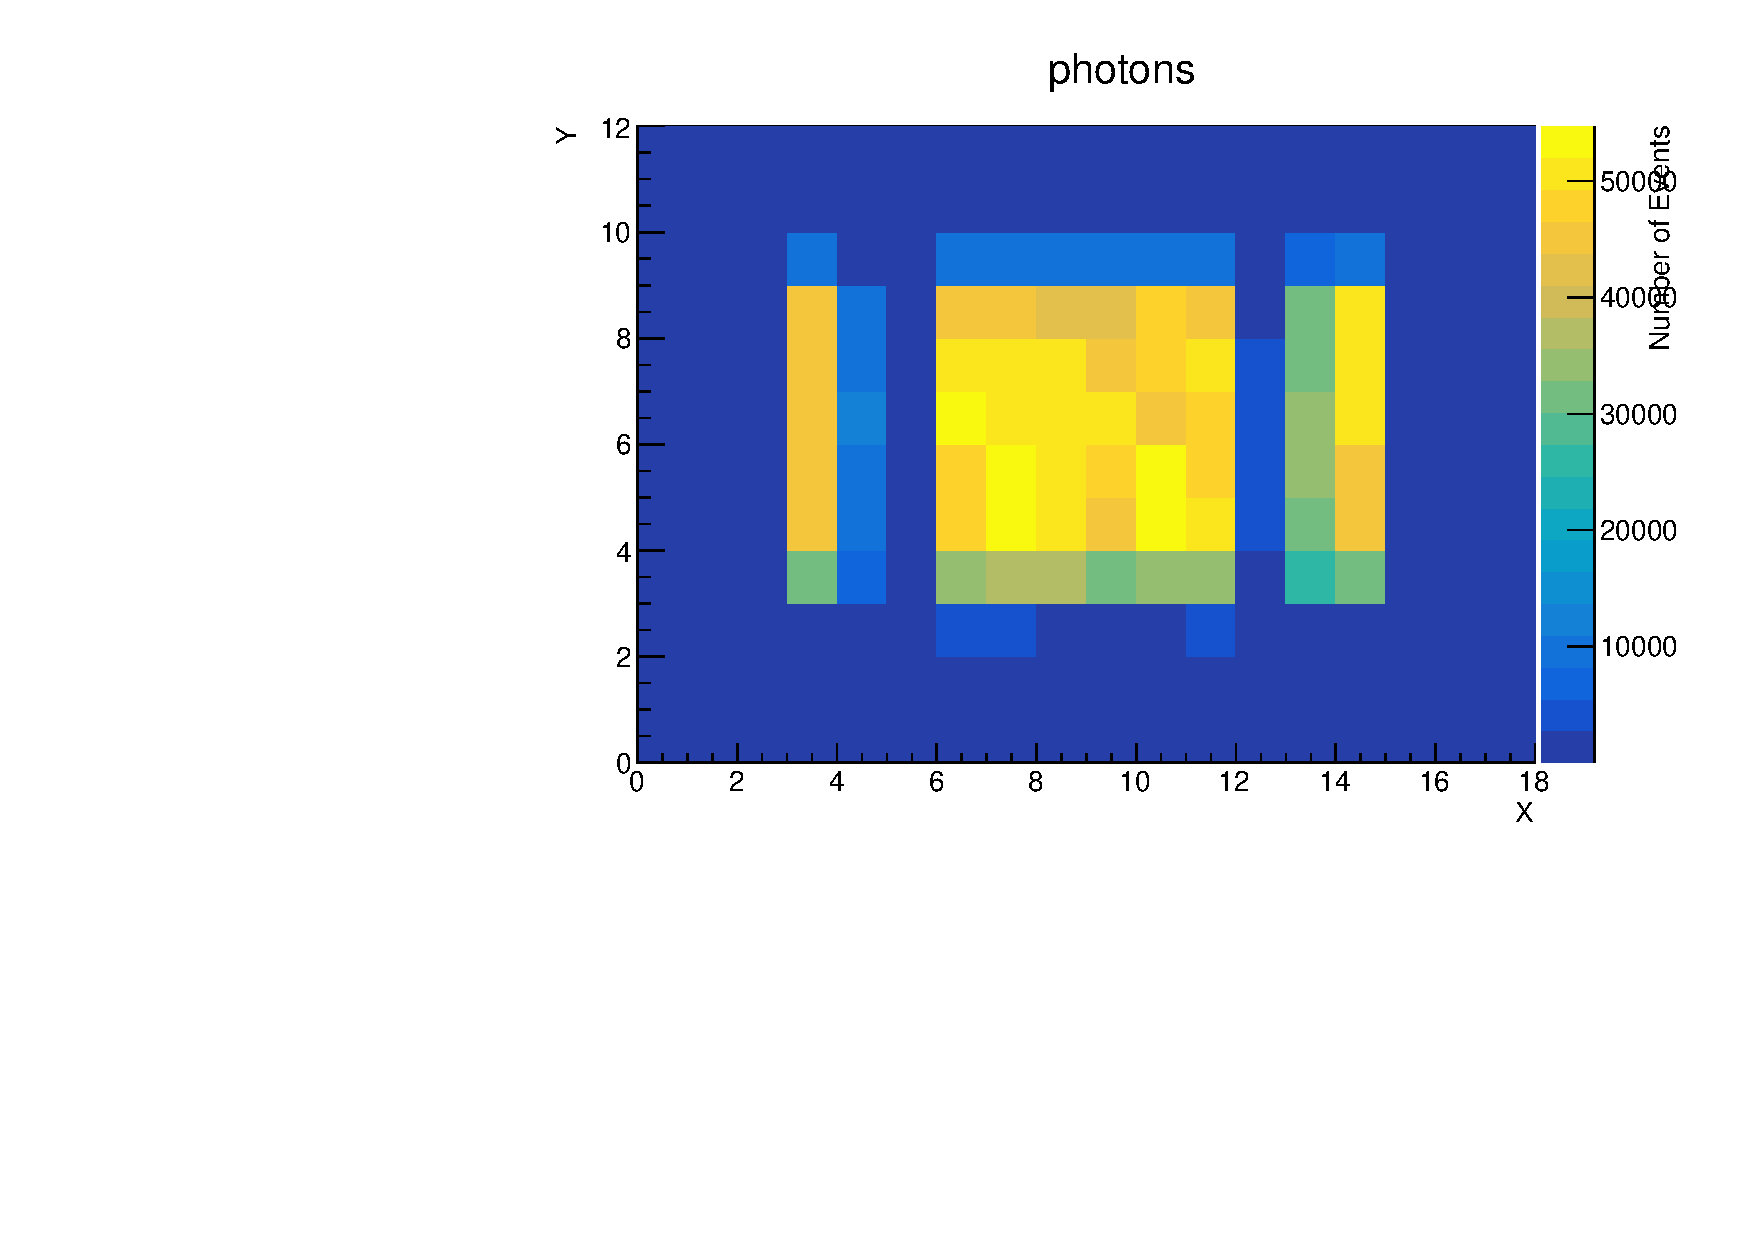
\includegraphics[scale=0.35]{Kap3/electron_scintillator_photons_plots_calo_counter.pdf}\label{fig:photons-creation-scintillator-1}}\hspace{1em}
  \subfloat[\(e^-\) as primary particle, Z axis of the calorimeter.]{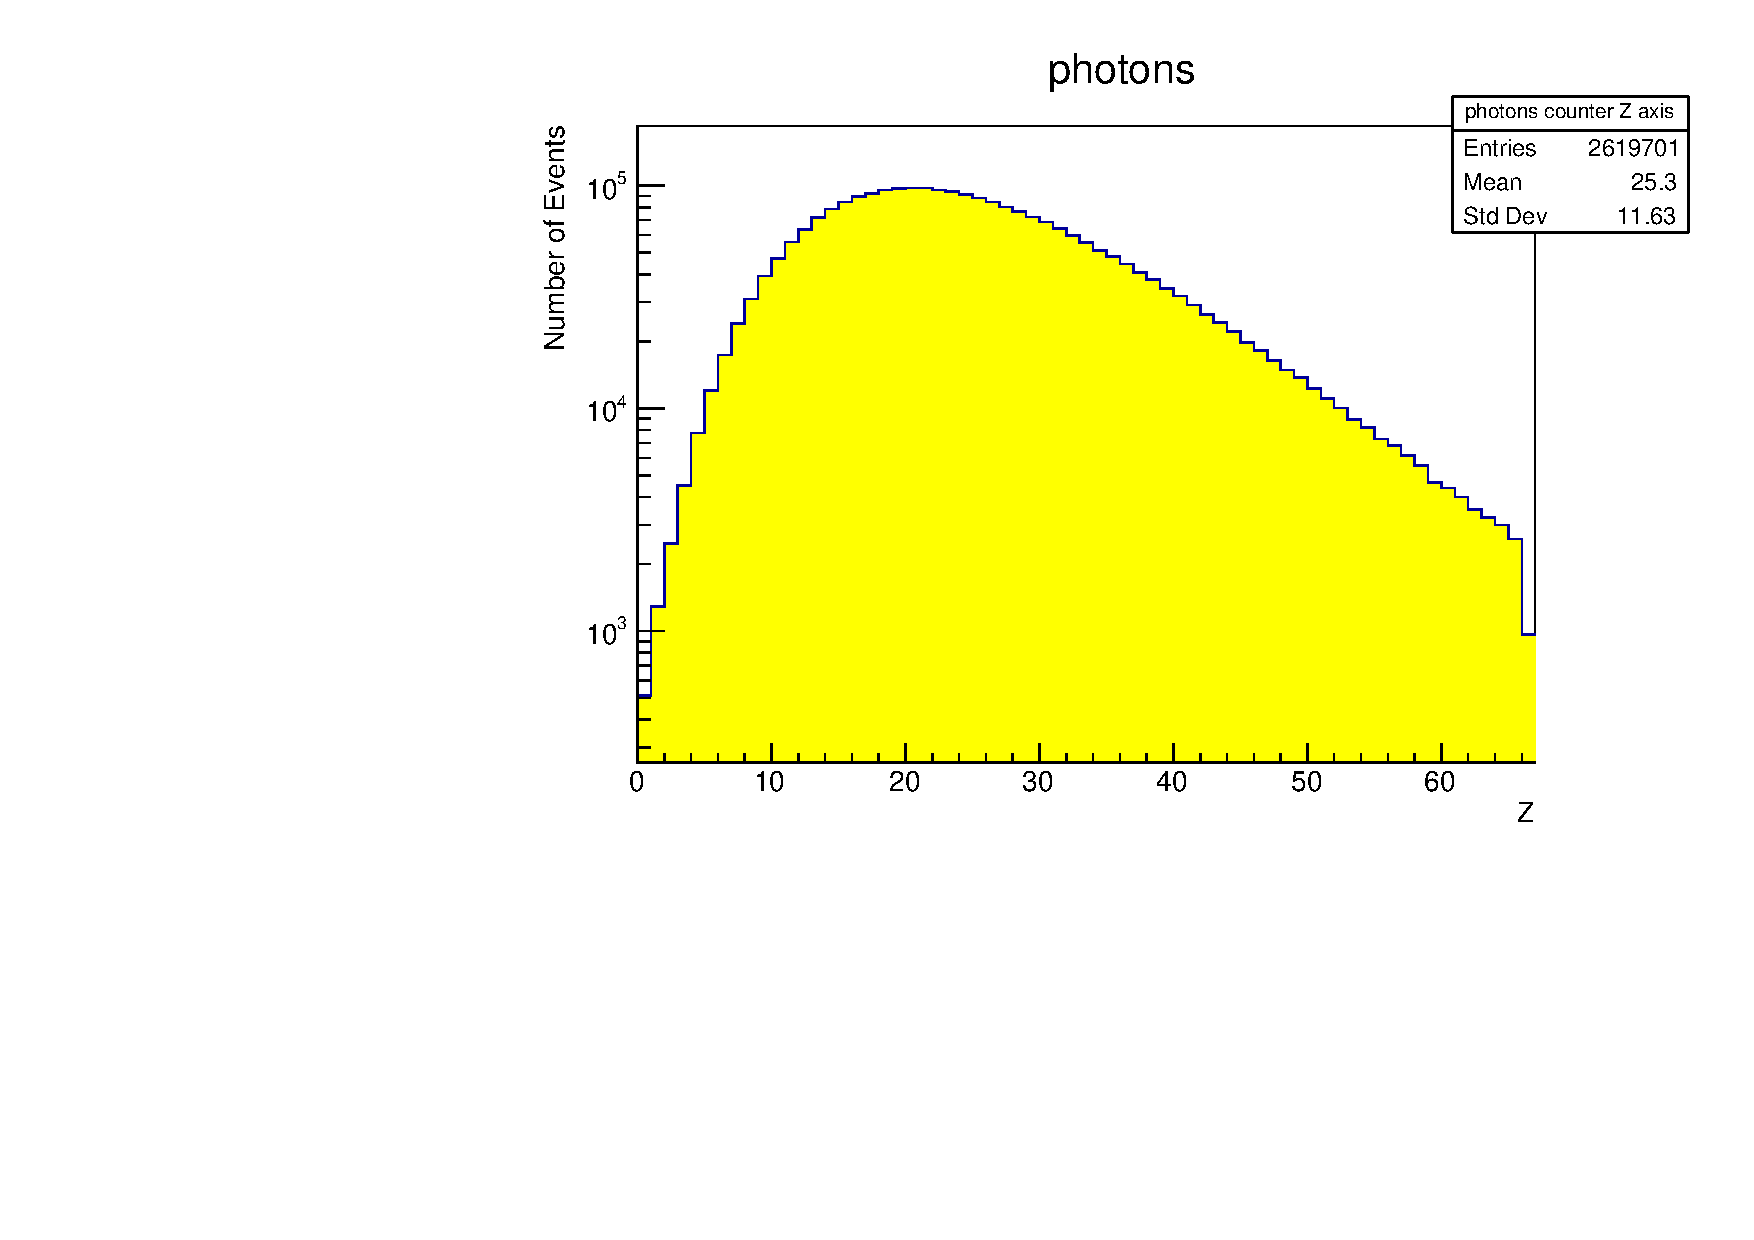
\includegraphics[scale=0.35]{Kap3/electron_scintillator_photons_plots_calo_counter_Z.pdf}\label{fig:photons-creation-scintillator-2}}

  \subfloat[\(\gamma\) as primary particle, X-Y plane of the calorimeter.]{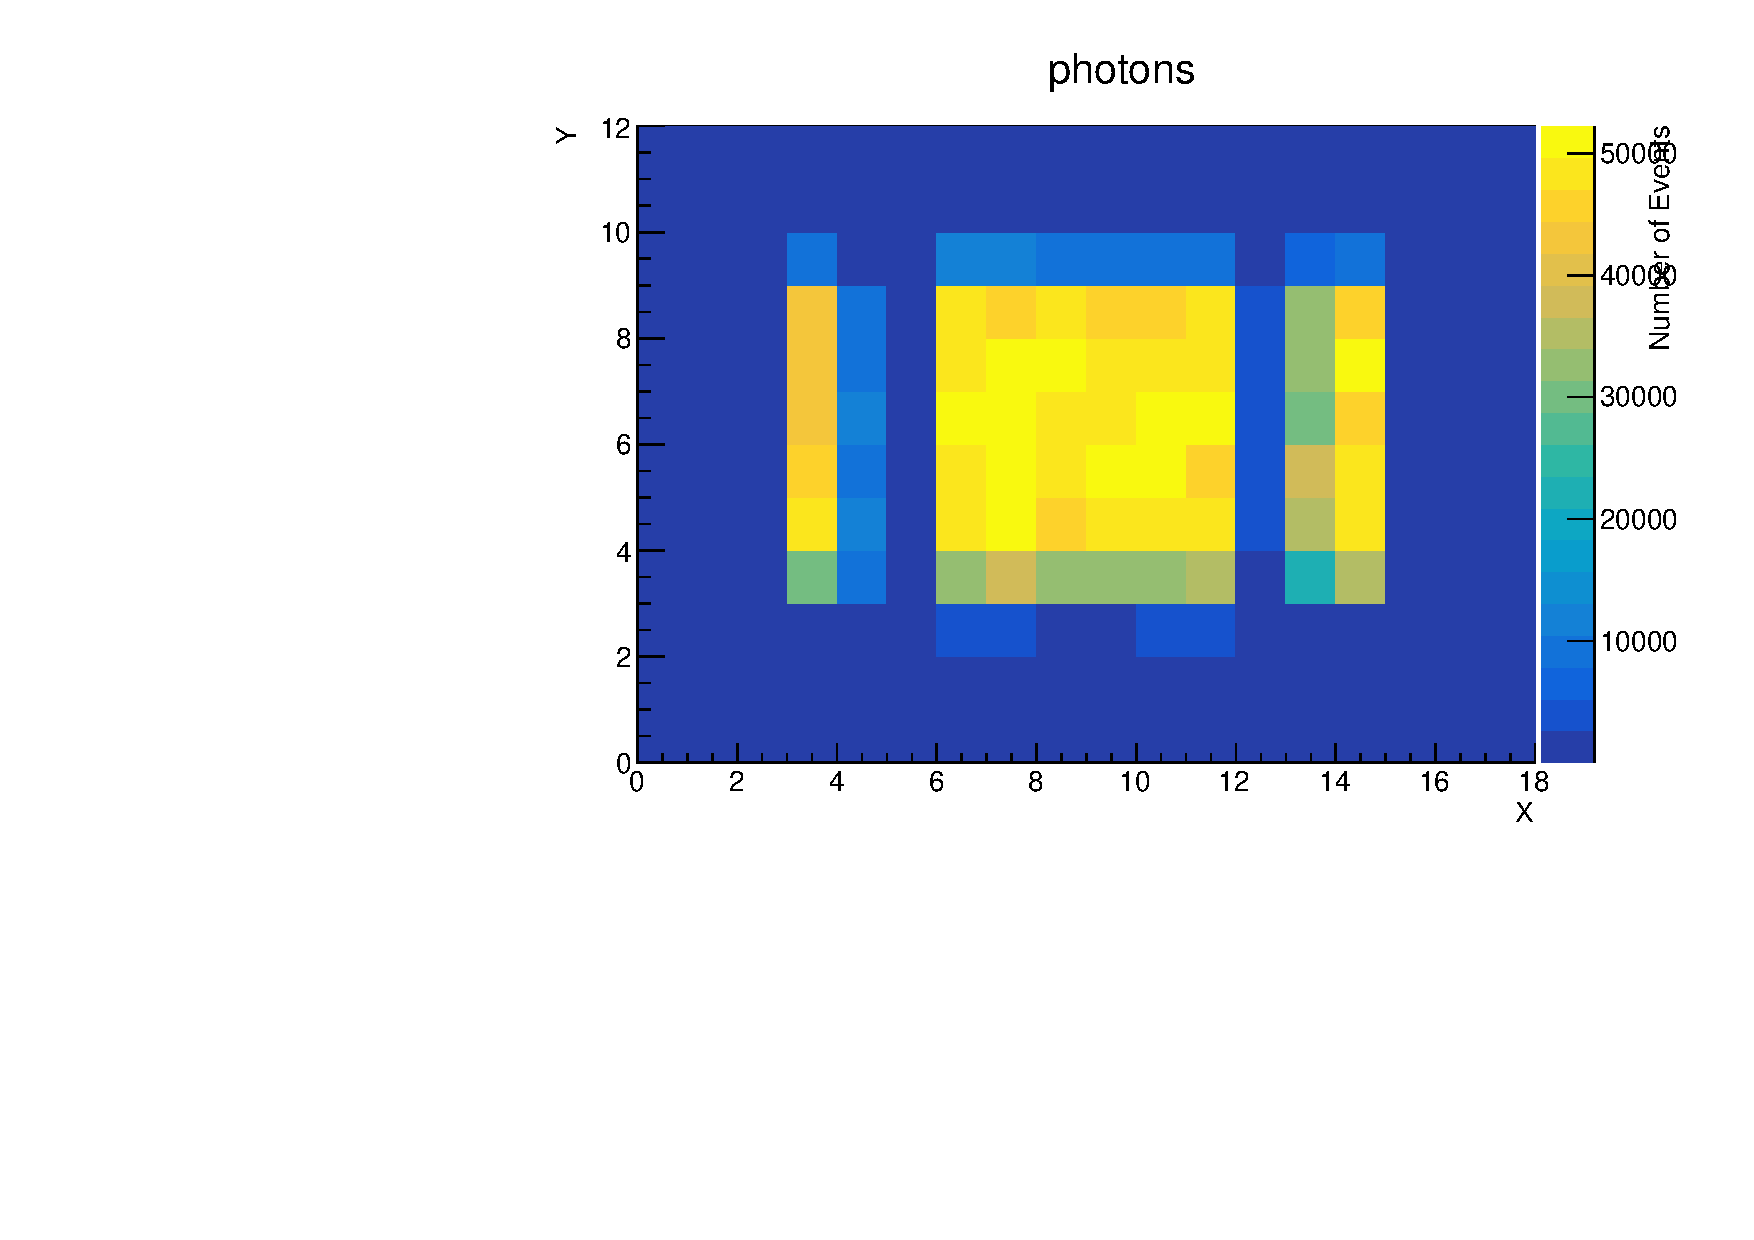
\includegraphics[scale=0.35]{Kap3/gamma_scintillator_photons_plots_calo_counter.pdf}\label{fig:photons-creation-scintillator-3}}\hspace{1em}
  \subfloat[\(\gamma\) as primary particle, Z axis of the calorimeter.]{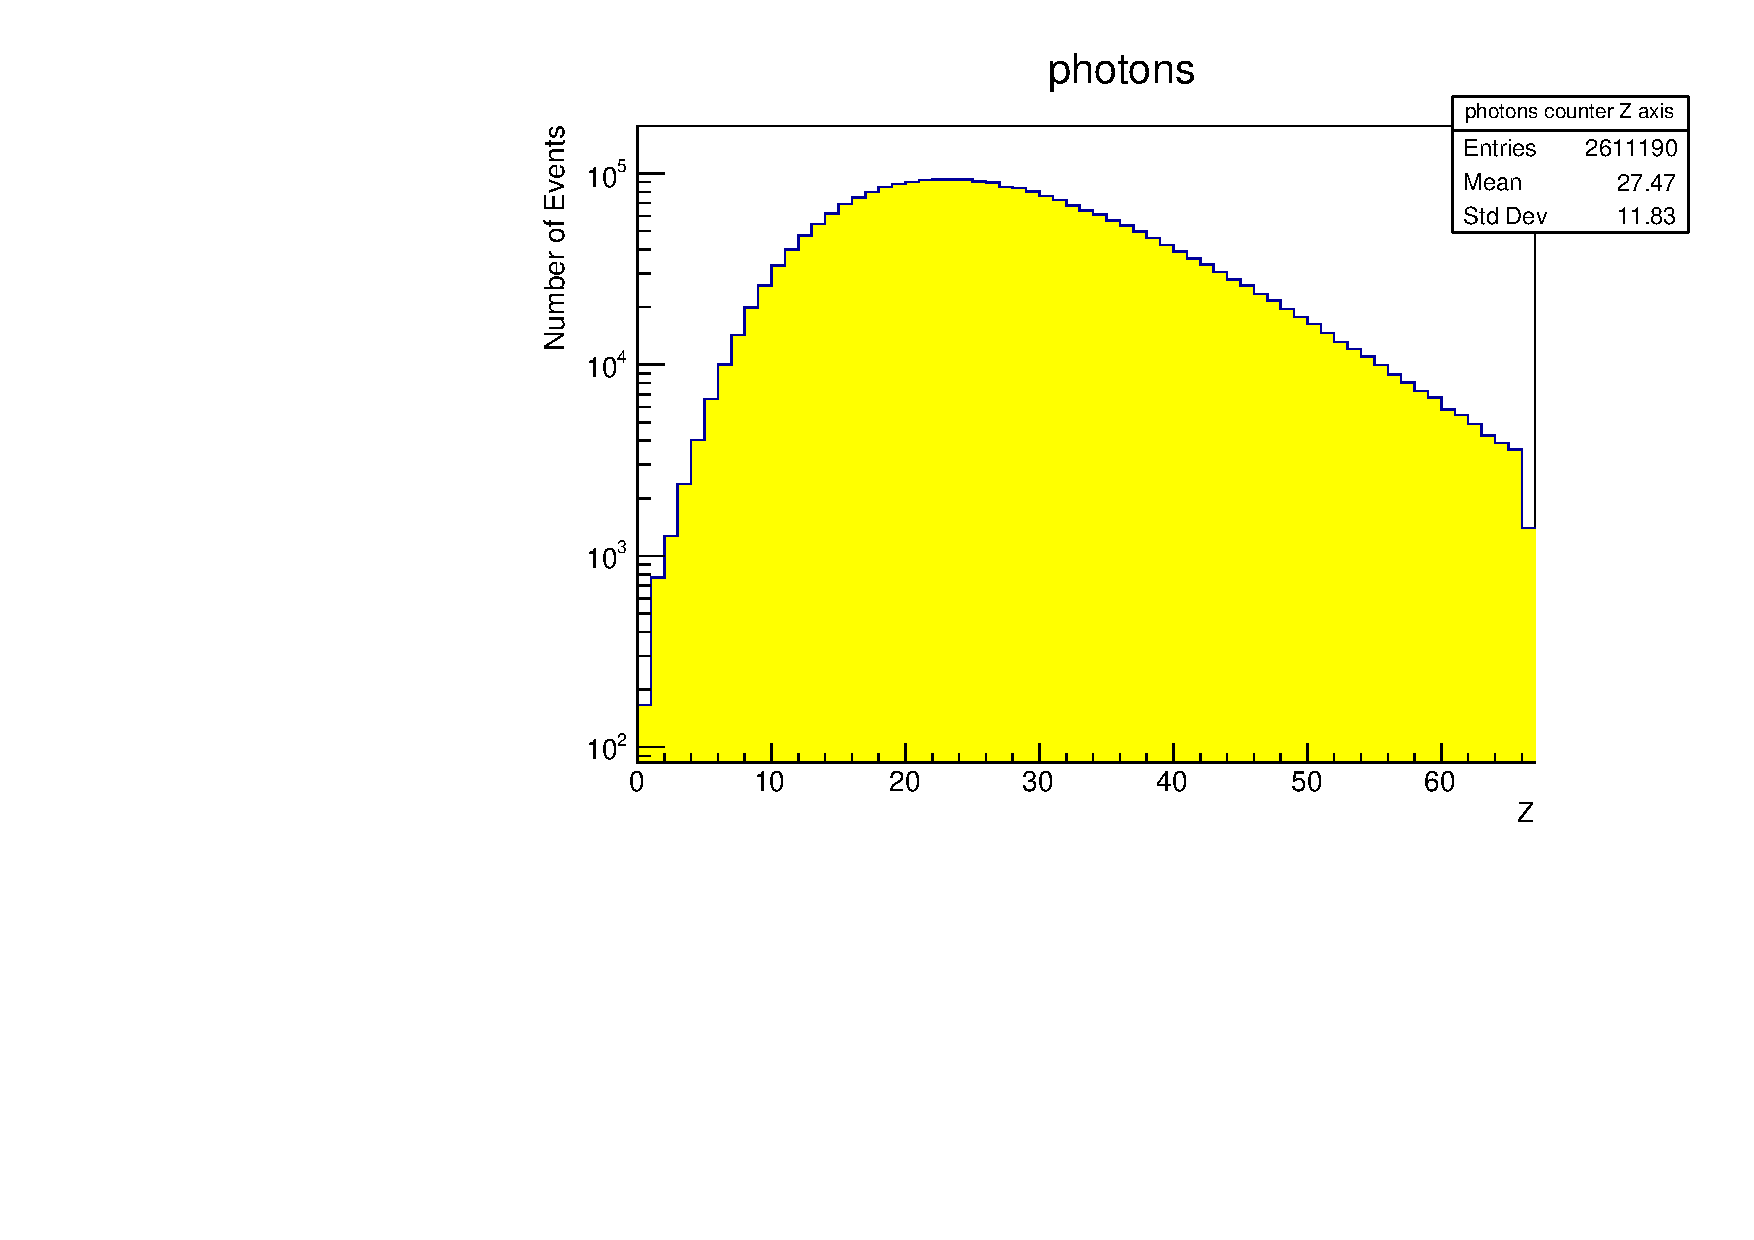
\includegraphics[scale=0.35]{Kap3/gamma_scintillator_photons_plots_calo_counter_Z.pdf}\label{fig:photons-creation-scintillator-4}}

  \subfloat[\(\pi^0\) as primary particle, X-Y plane of the calorimeter.]{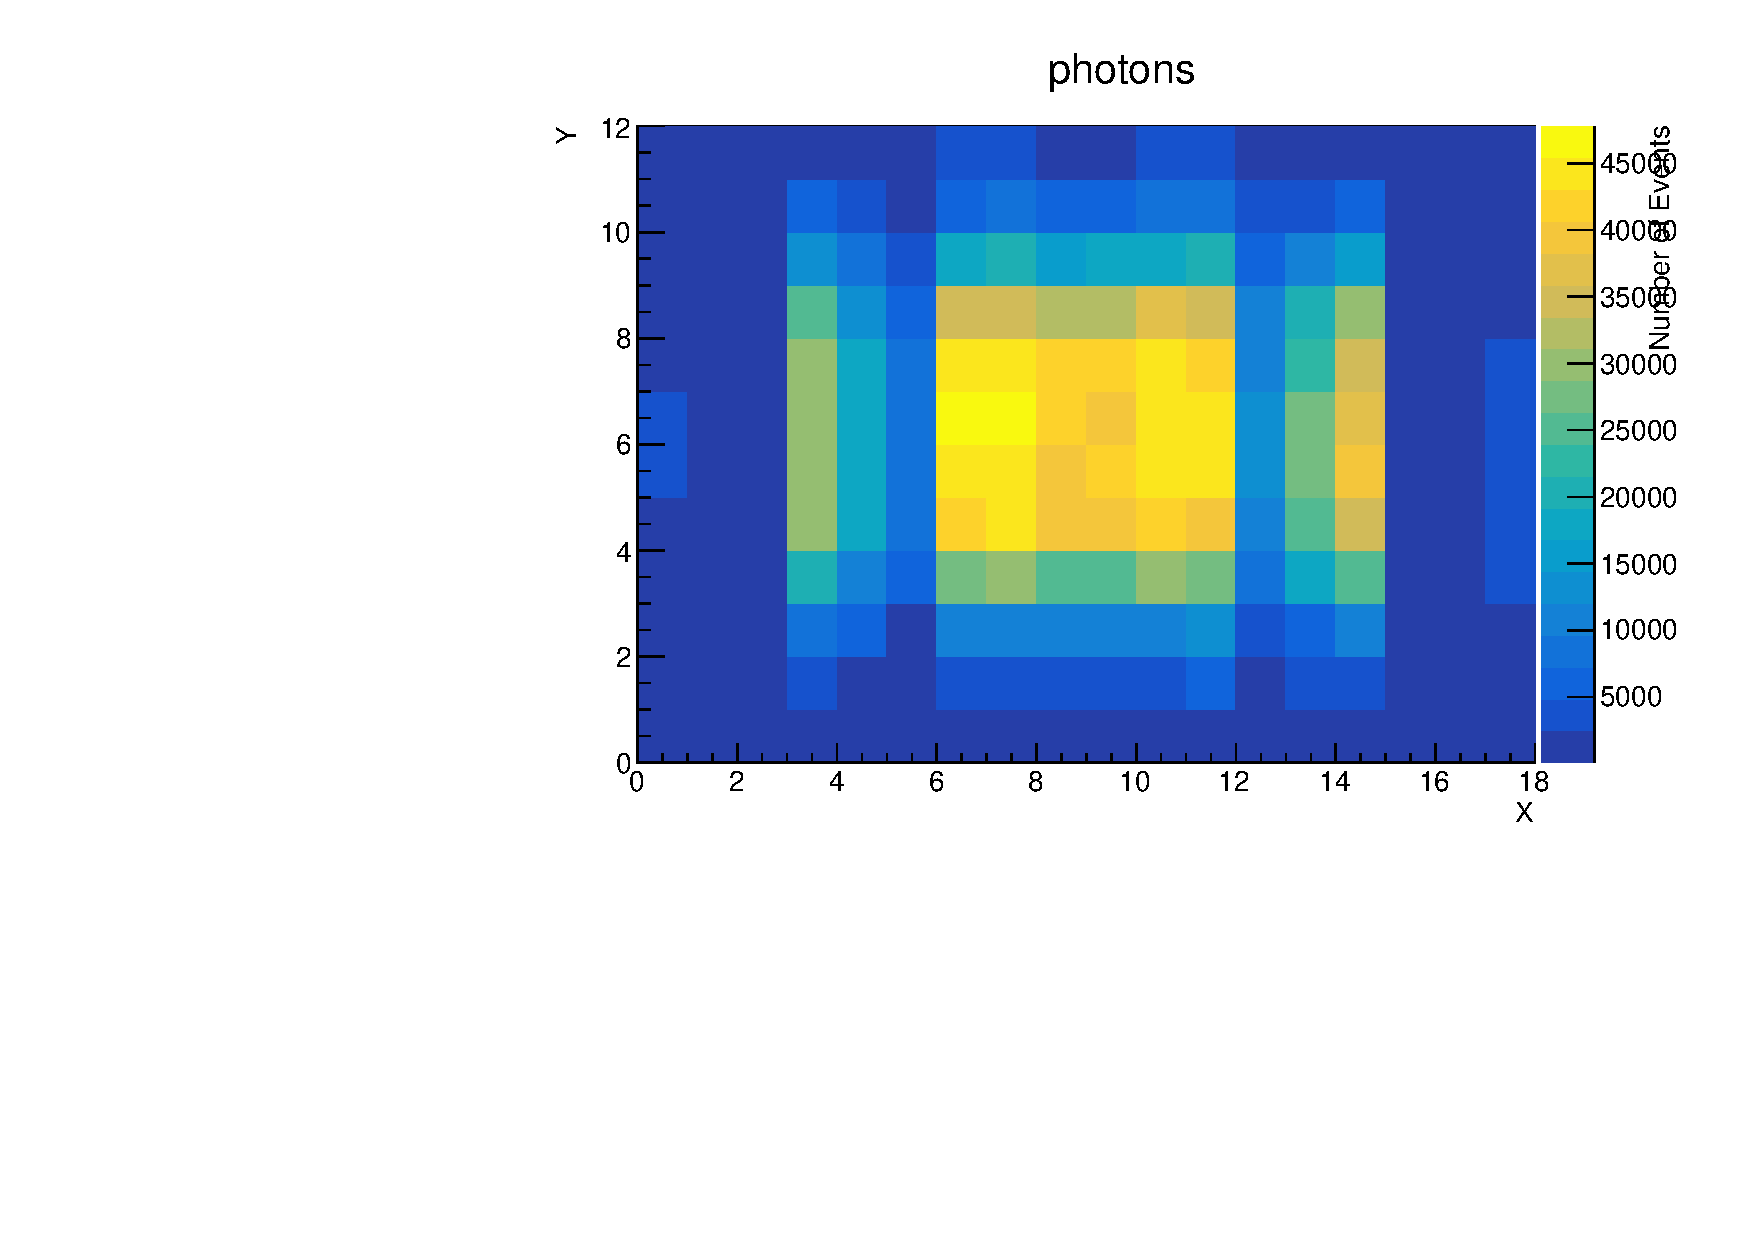
\includegraphics[scale=0.35]{Kap3/pi0_scintillator_photons_plots_calo_counter.pdf}\label{fig:photons-creation-scintillator-5}}\hspace{1em}
  \subfloat[\(\pi^0\) as primary particle, Z axis of the calorimeter.]{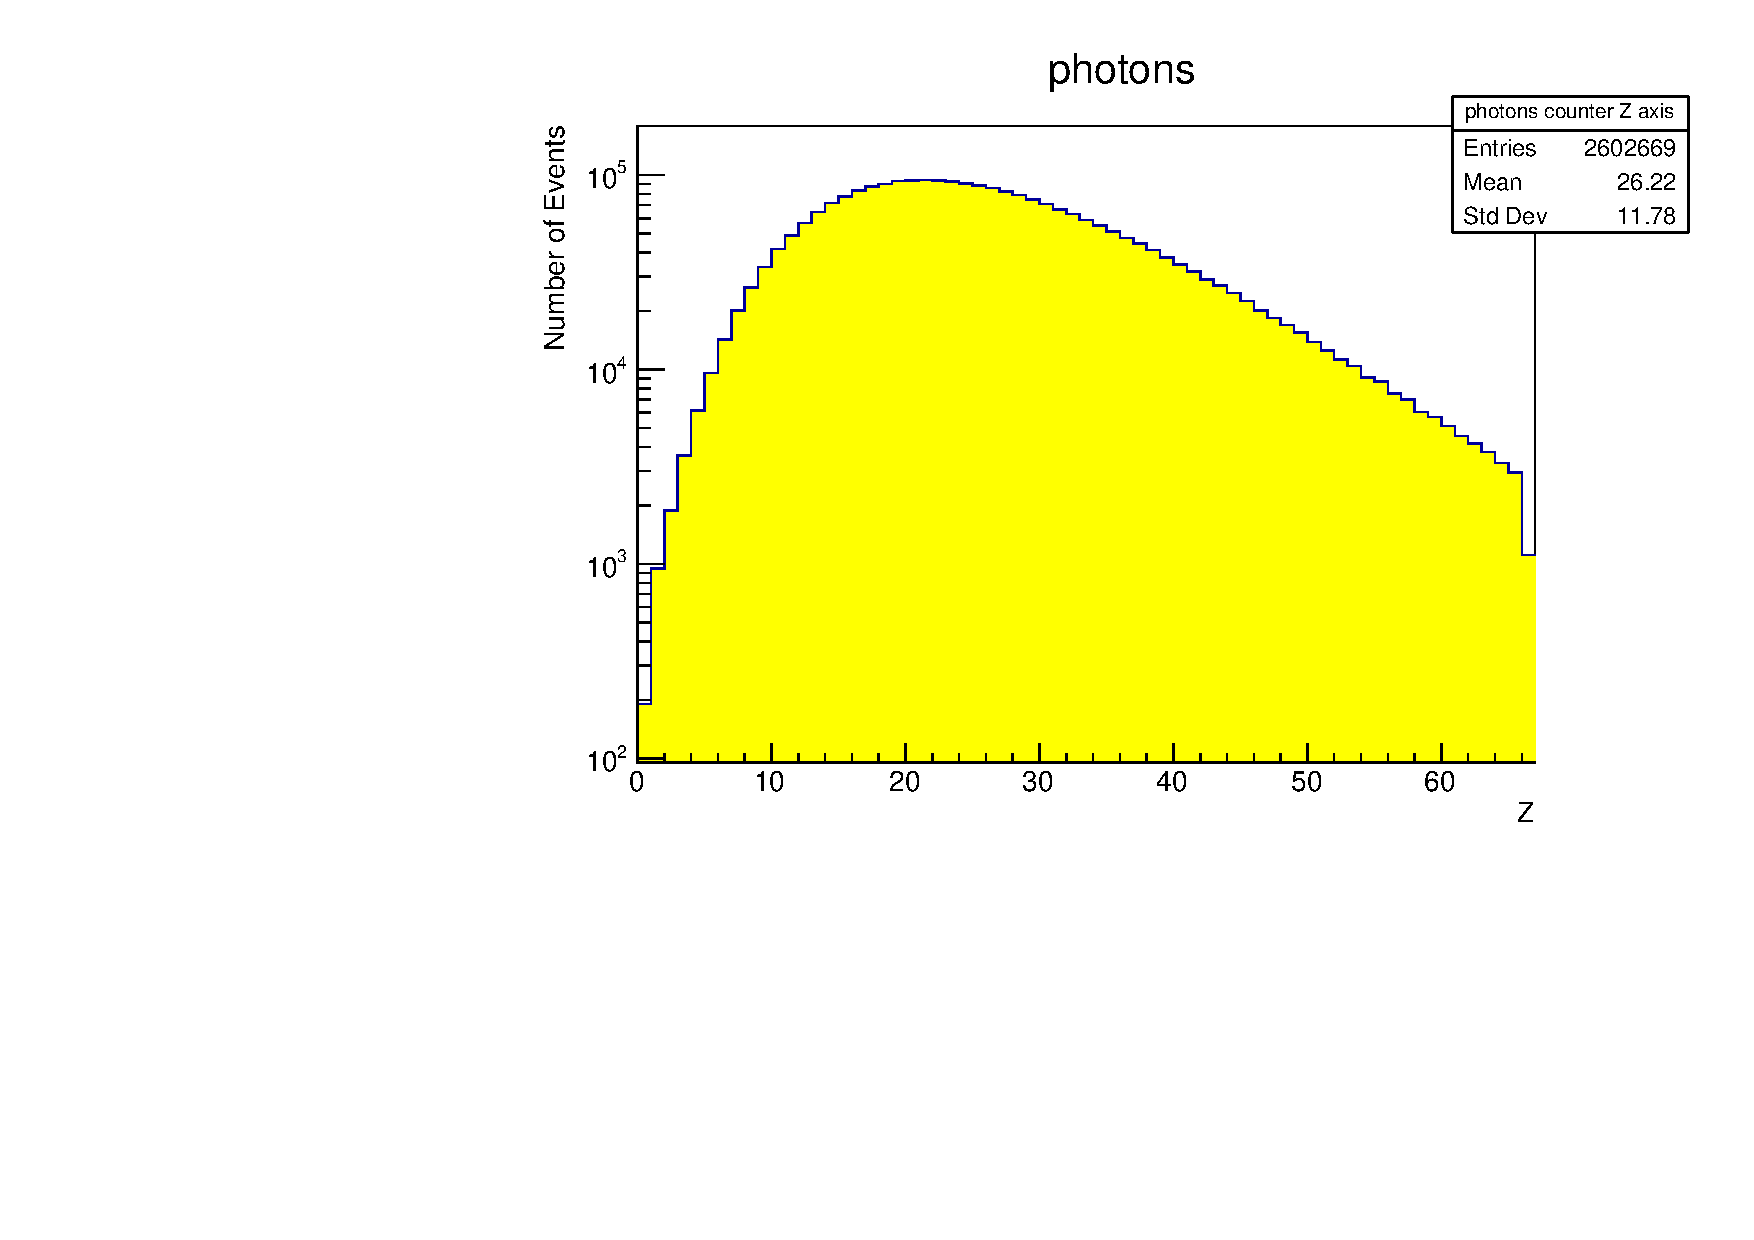
\includegraphics[scale=0.35]{Kap3/pi0_scintillator_photons_plots_calo_counter_Z.pdf}\label{fig:photons-creation-scintillator-6}}

  \caption{Photons creation in the scintillator plates of the calorimeter.}\label{fig:photons-creation-scintillator}

\end{figure}

Let's start with the photon creation in the scintillator plates, as show in the
\cref{fig:photons-creation-scintillator}. In the X-Y plane the mean is at
\((8.777, 5.695)\), \((8.797, 5.702)\) and \(8.755, 5.708\) for electrons,
photons and neutral pions events respectively. In general, the mean value lays
in the center of the mesh. The only noticeable difference is in the standard
deviation that can be seen in the number of events outside the central plates.
The pion signal have a standard deviation of \((3.398, 2.183)\) being larger
than that of electrons of \((3.266, 1.801)\) and photons of \((3.270, 1.805)\),
highlighting that the greatest difference is in the standard deviation of the
vertical axis.

\begin{figure}[htb!]
  \centering

  \subfloat[\(e^-\) as primary particle, X-Y plane of the calorimeter.]{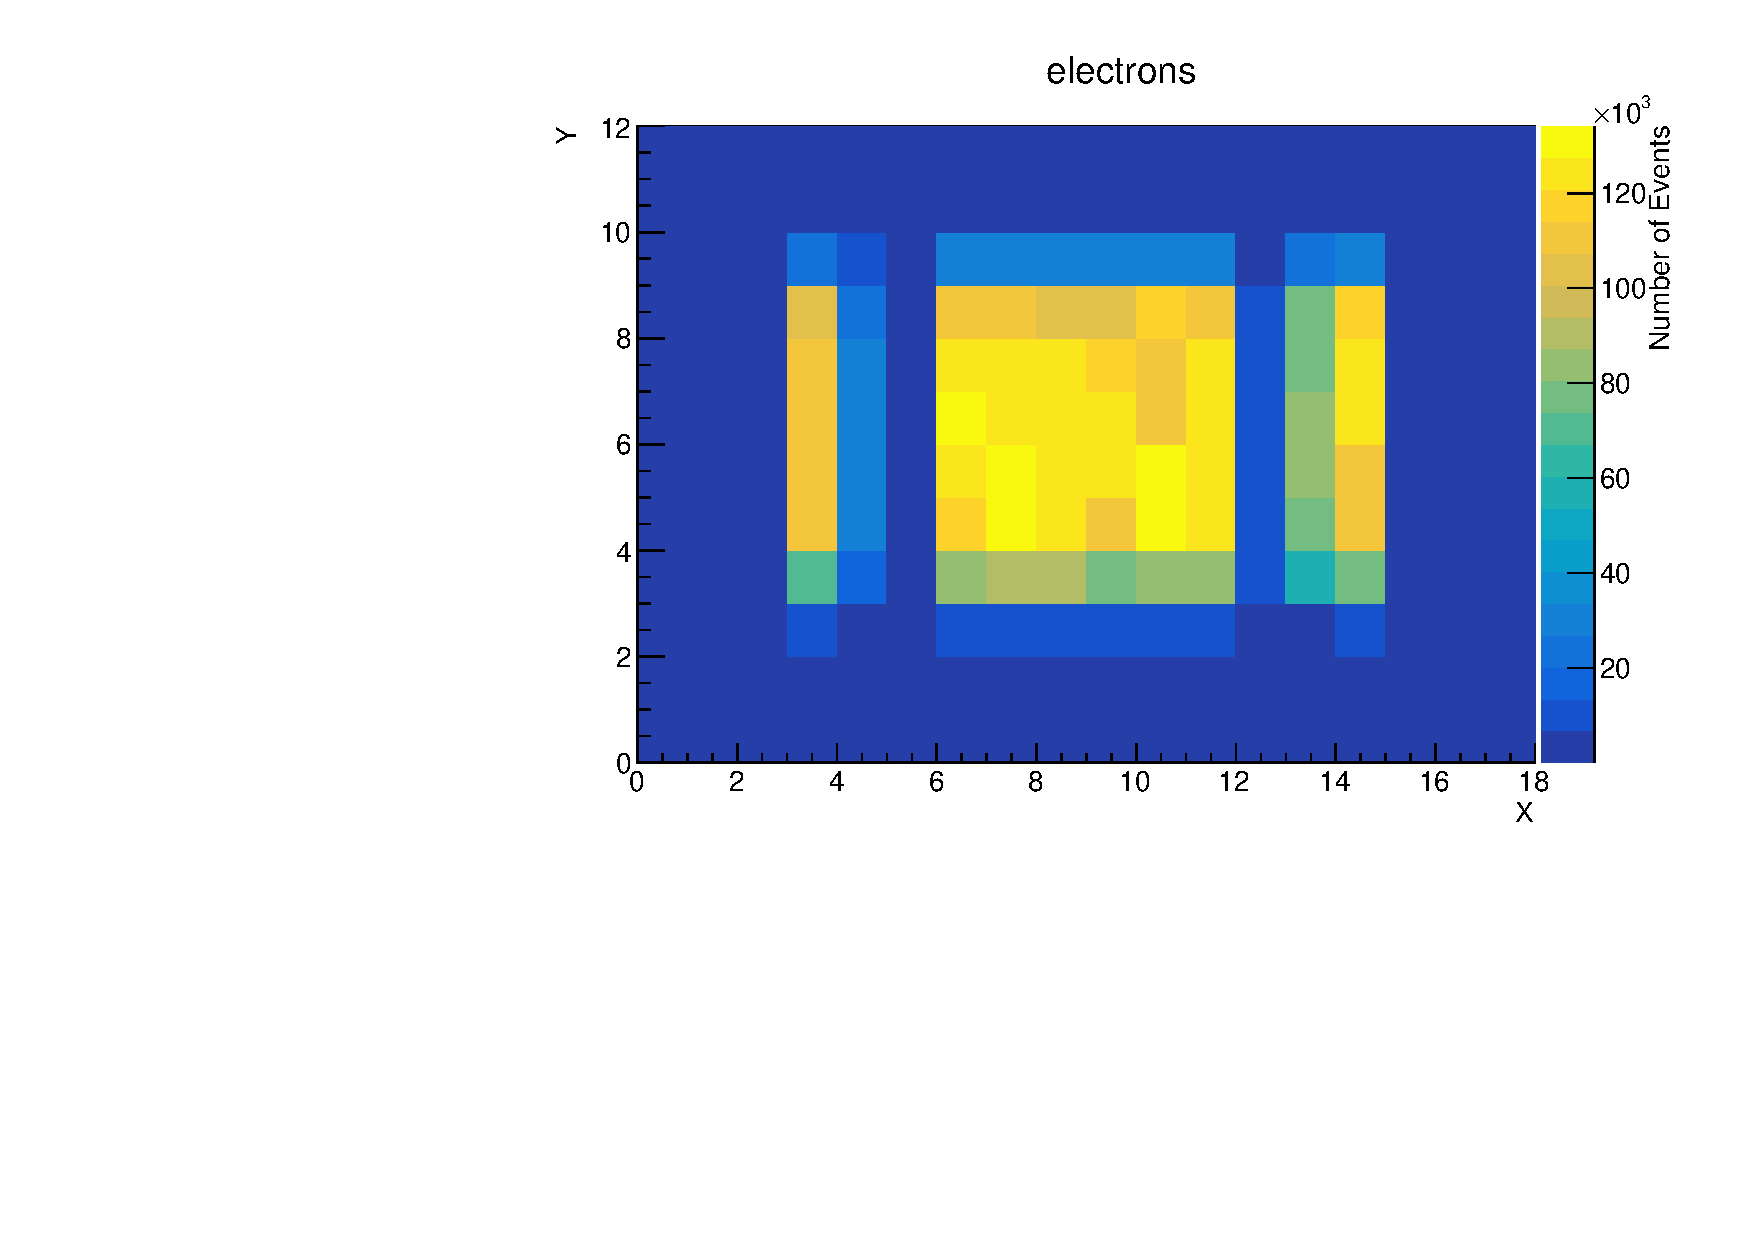
\includegraphics[scale=0.35]{Kap3/electron_scintillator_electrons_plots_calo_counter.pdf}\label{fig:electrons-creation-scintillator-1}}\hspace{1em}
  \subfloat[\(e^-\) as primary particle, Z axis
   of the calorimeter.]{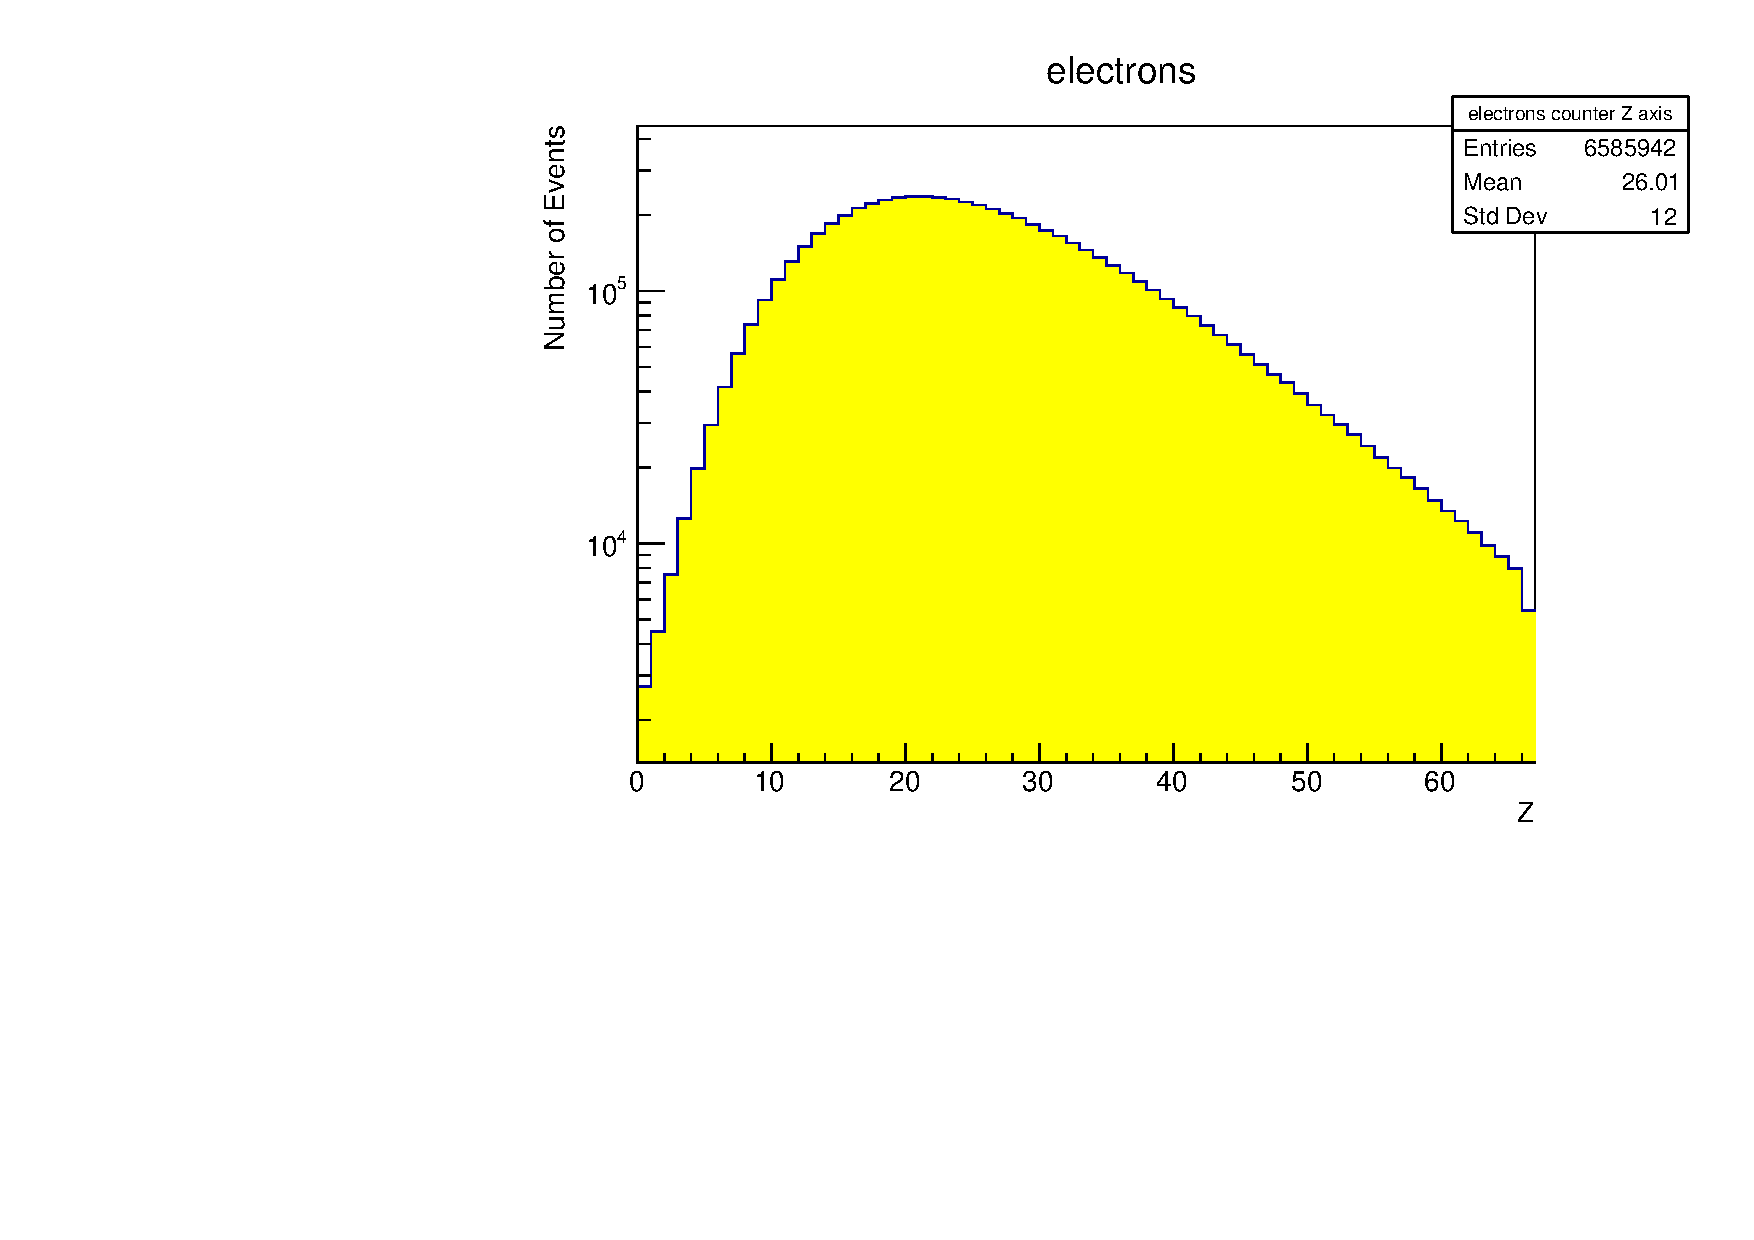
\includegraphics[scale=0.35]{Kap3/electron_scintillator_electrons_plots_calo_counter_Z.pdf}\label{fig:electrons-creation-scintillator-2}}

   \subfloat[\(\gamma\) as primary particle, X-Y plane of the calorimeter.]{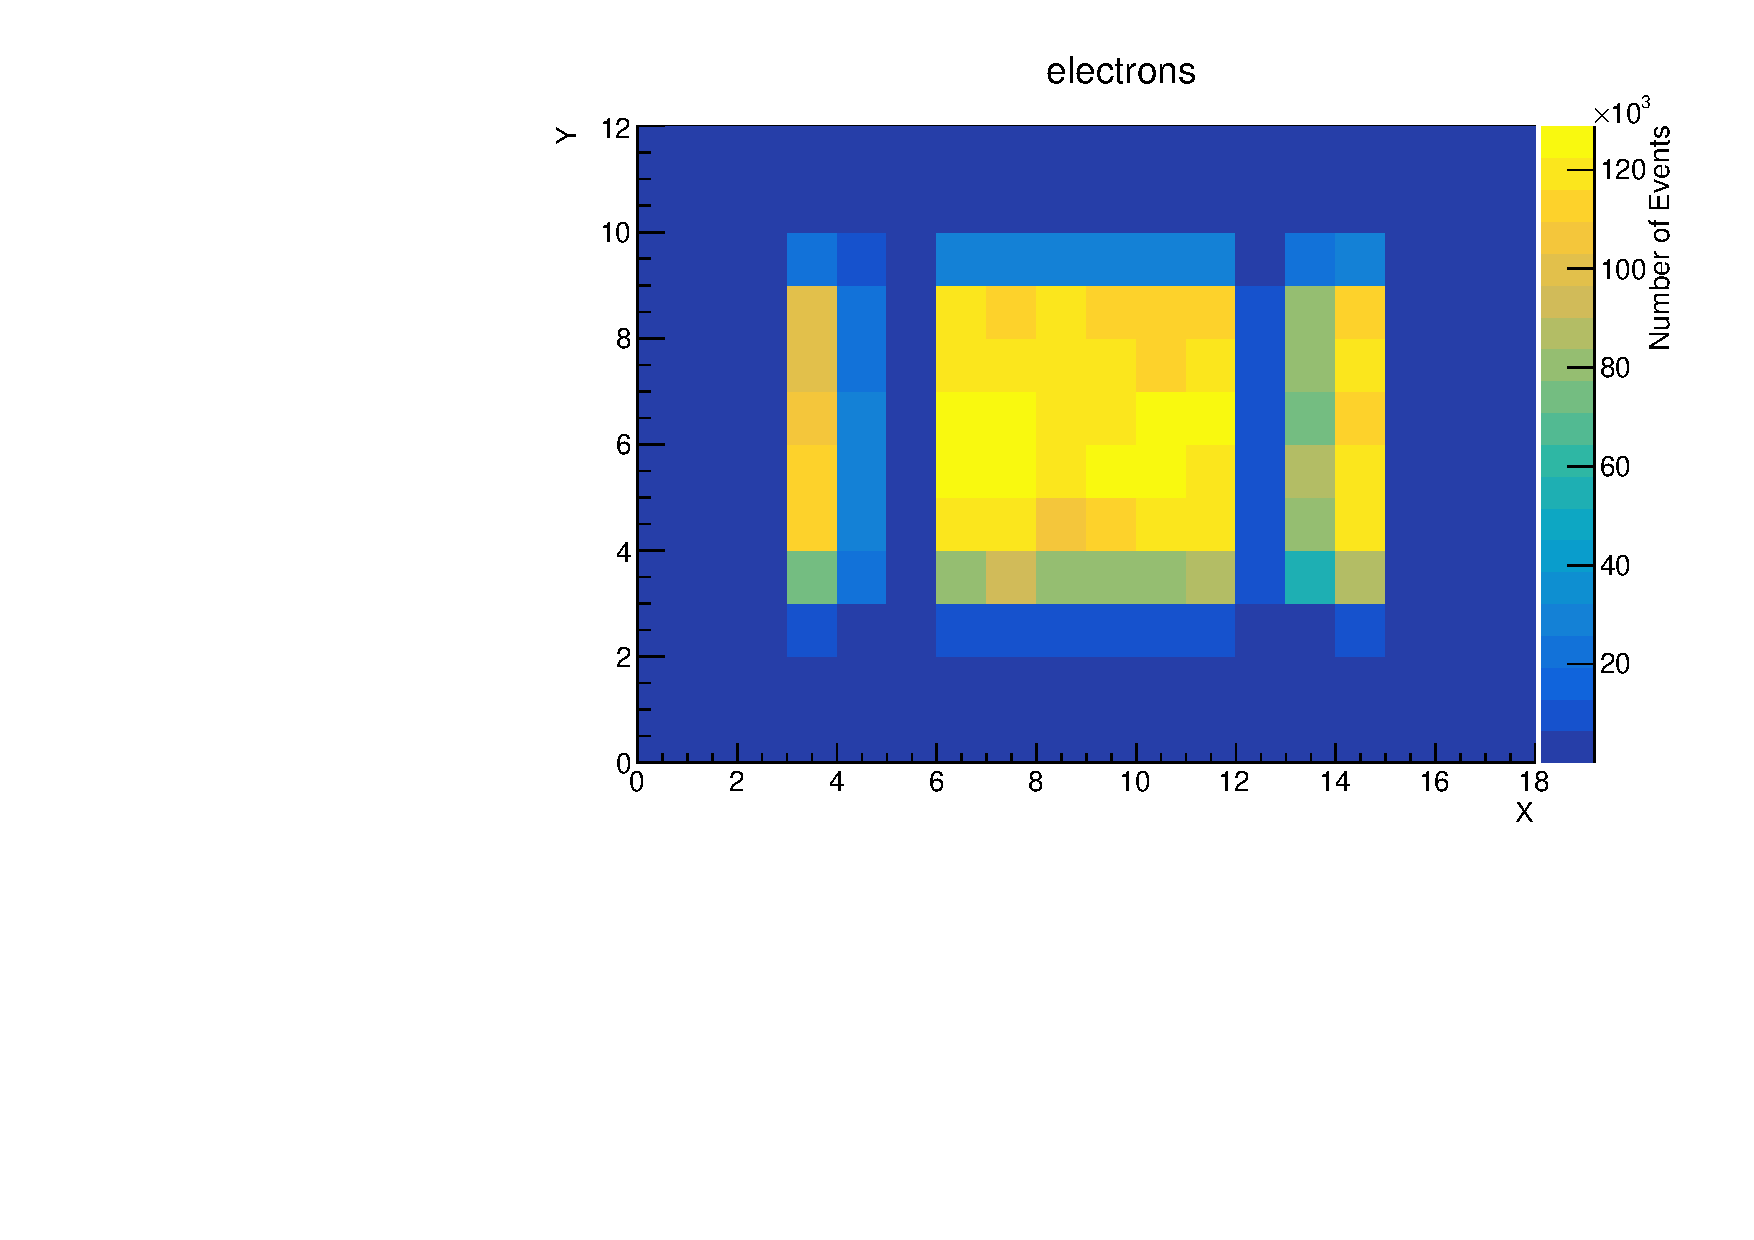
\includegraphics[scale=0.35]{Kap3/gamma_scintillator_electrons_plots_calo_counter.pdf}\label{fig:electrons-creation-scintillator-3}}\hspace{1em}
   \subfloat[\(\gamma\) as primary particle, Z axis of the calorimeter.]{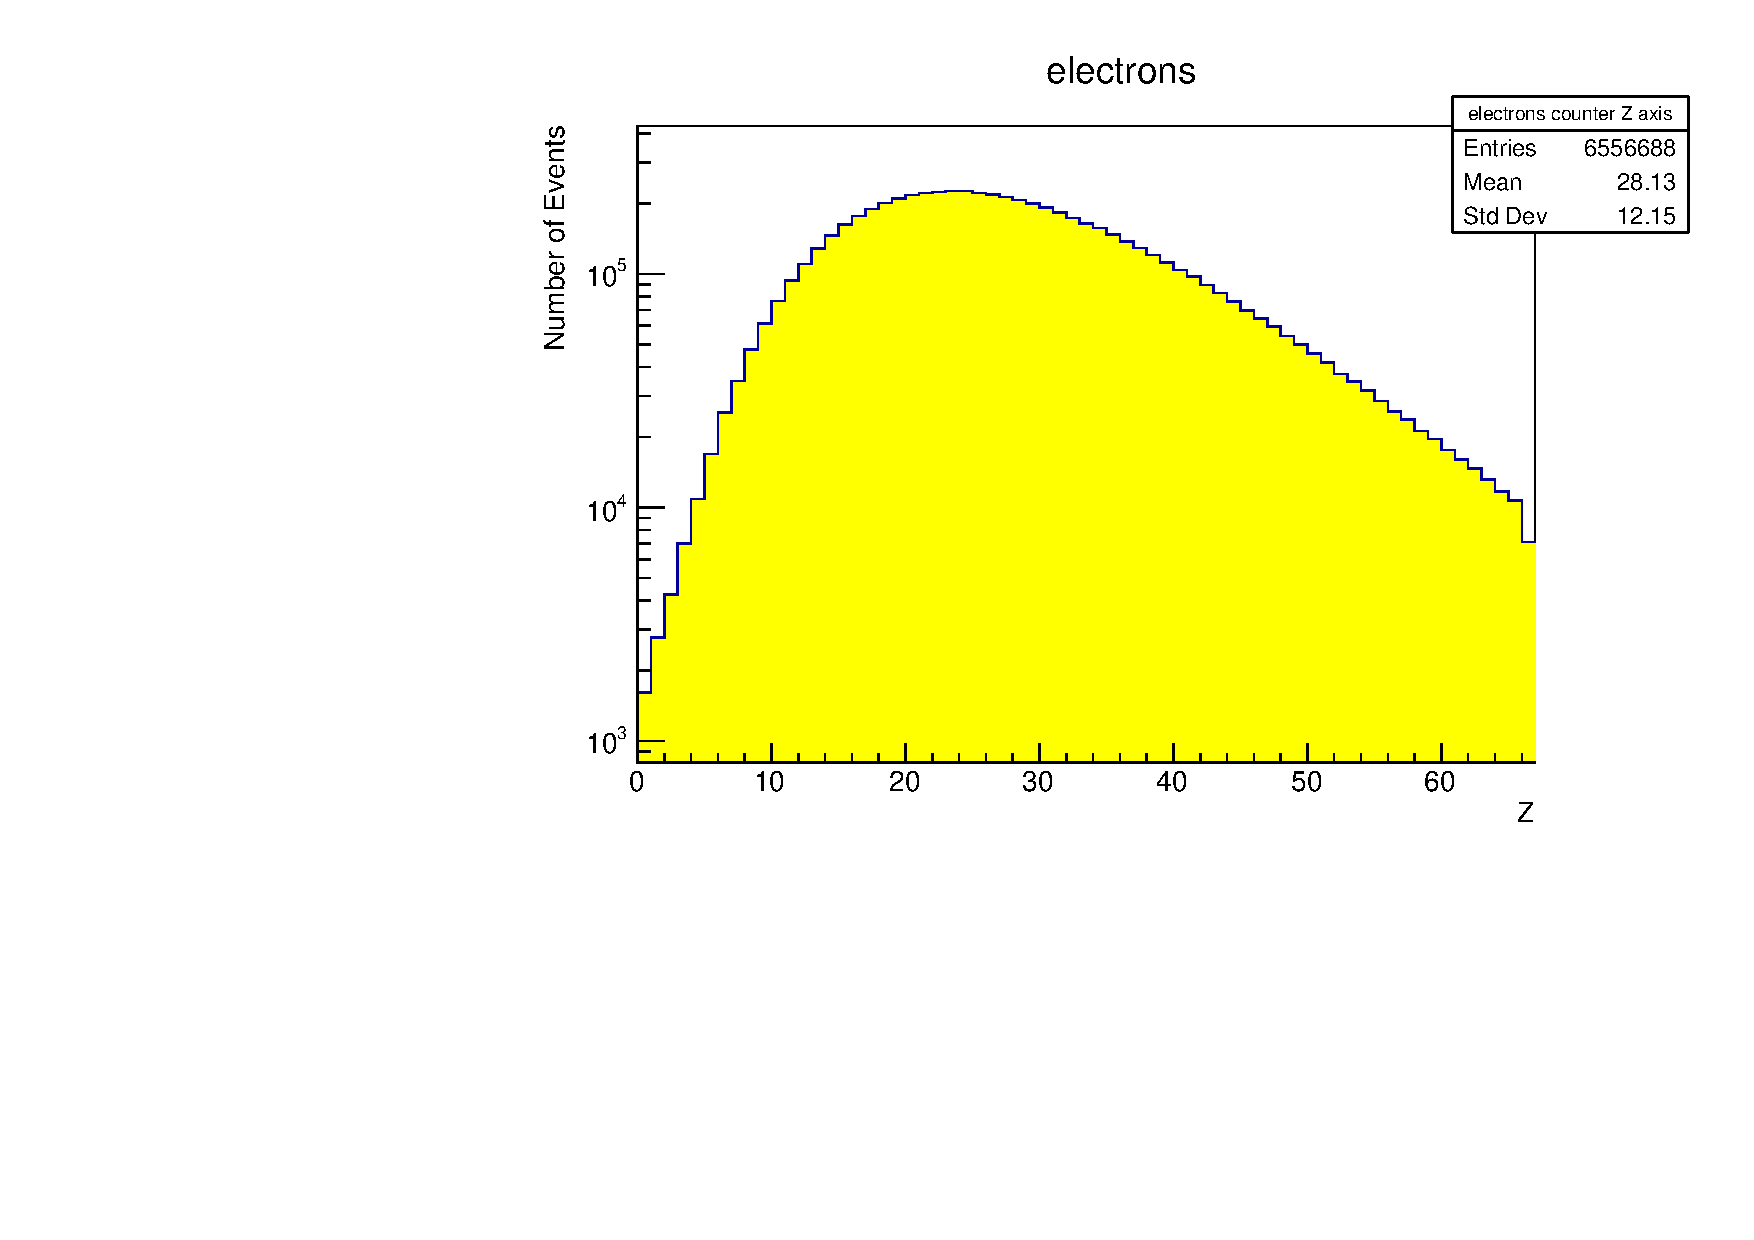
\includegraphics[scale=0.35]{Kap3/gamma_scintillator_electrons_plots_calo_counter_Z.pdf}\label{fig:electrons-creation-scintillator-4}}

   \subfloat[\(\pi^0\) as primary particle, X-Y plane of the calorimeter.]{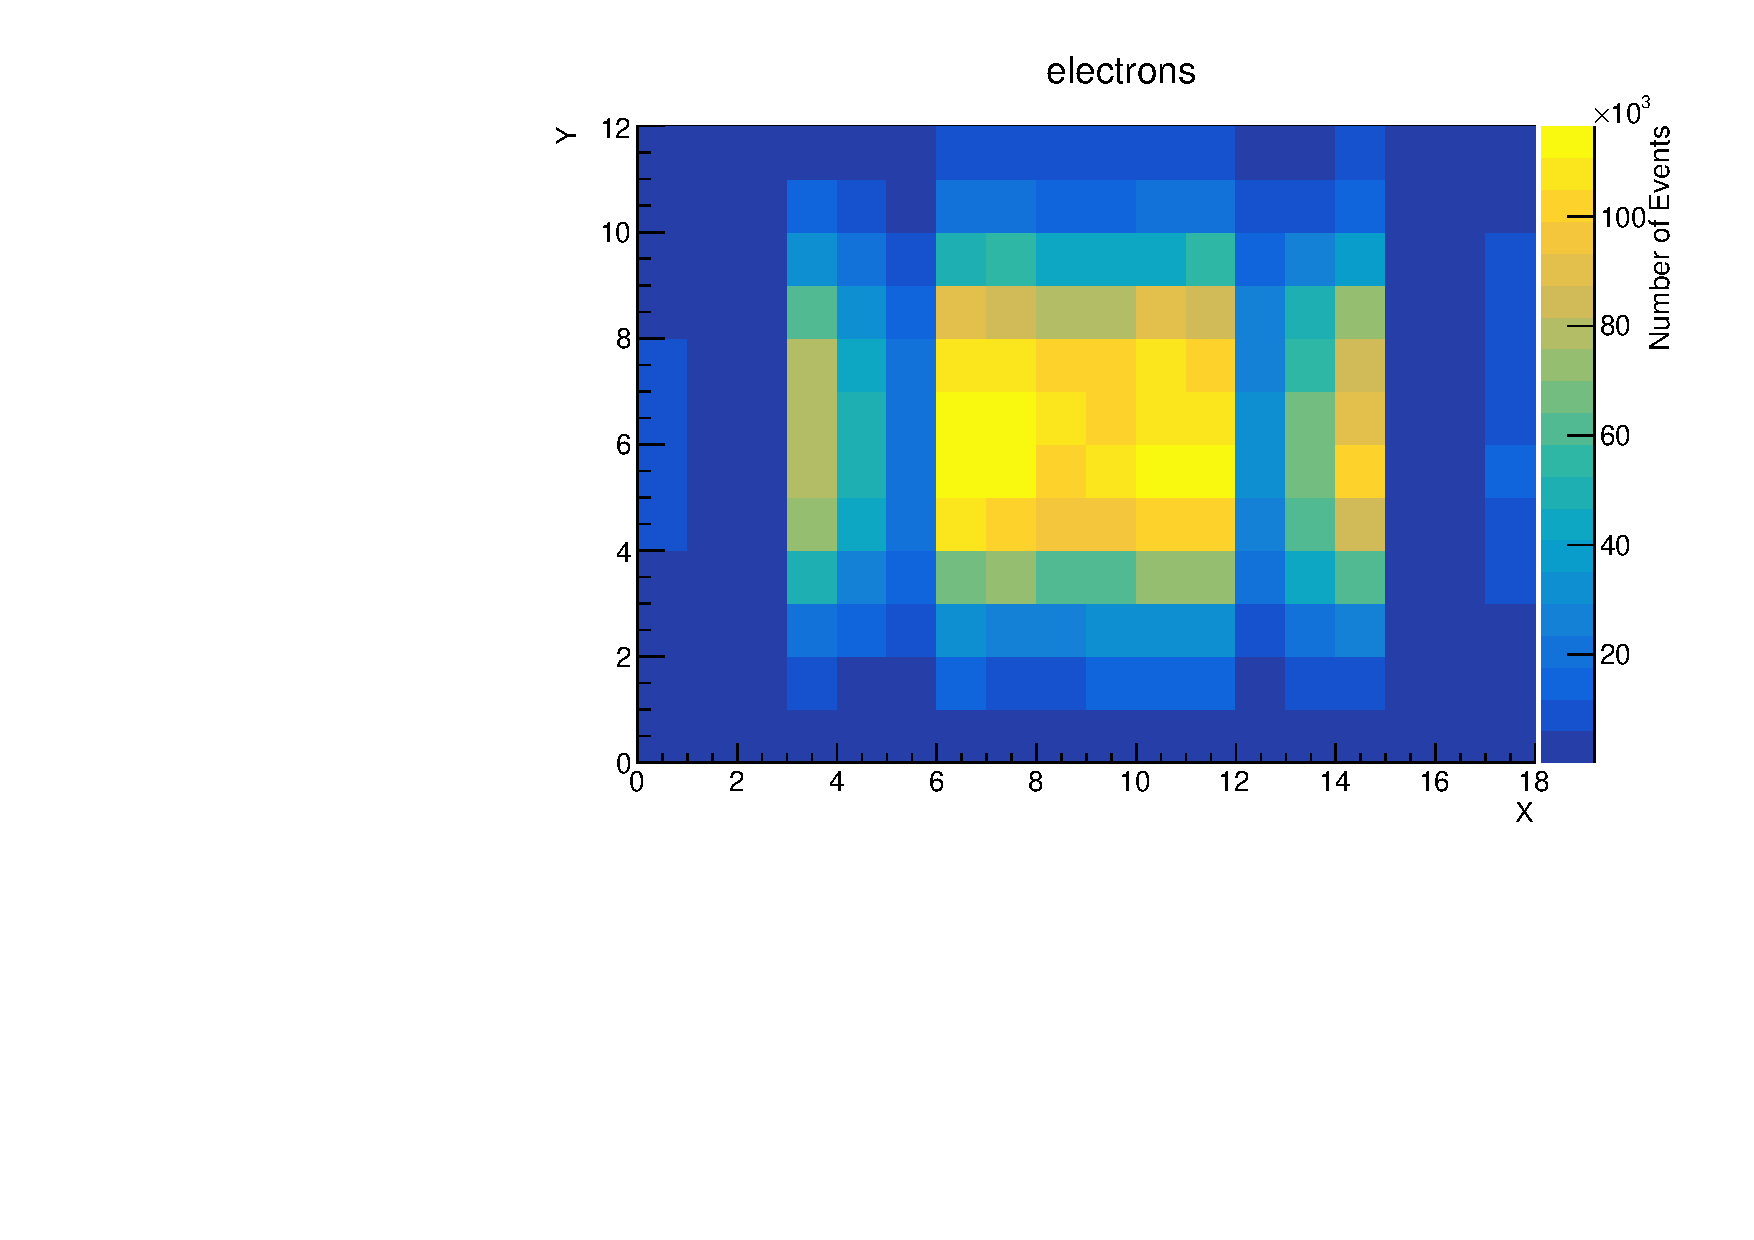
\includegraphics[scale=0.35]{Kap3/pi0_scintillator_electrons_plots_calo_counter.pdf}\label{fig:electrons-creation-scintillator-5}}\hspace{1em}
   \subfloat[\(\pi^0\) as primary particle, Z axis of the calorimeter.]{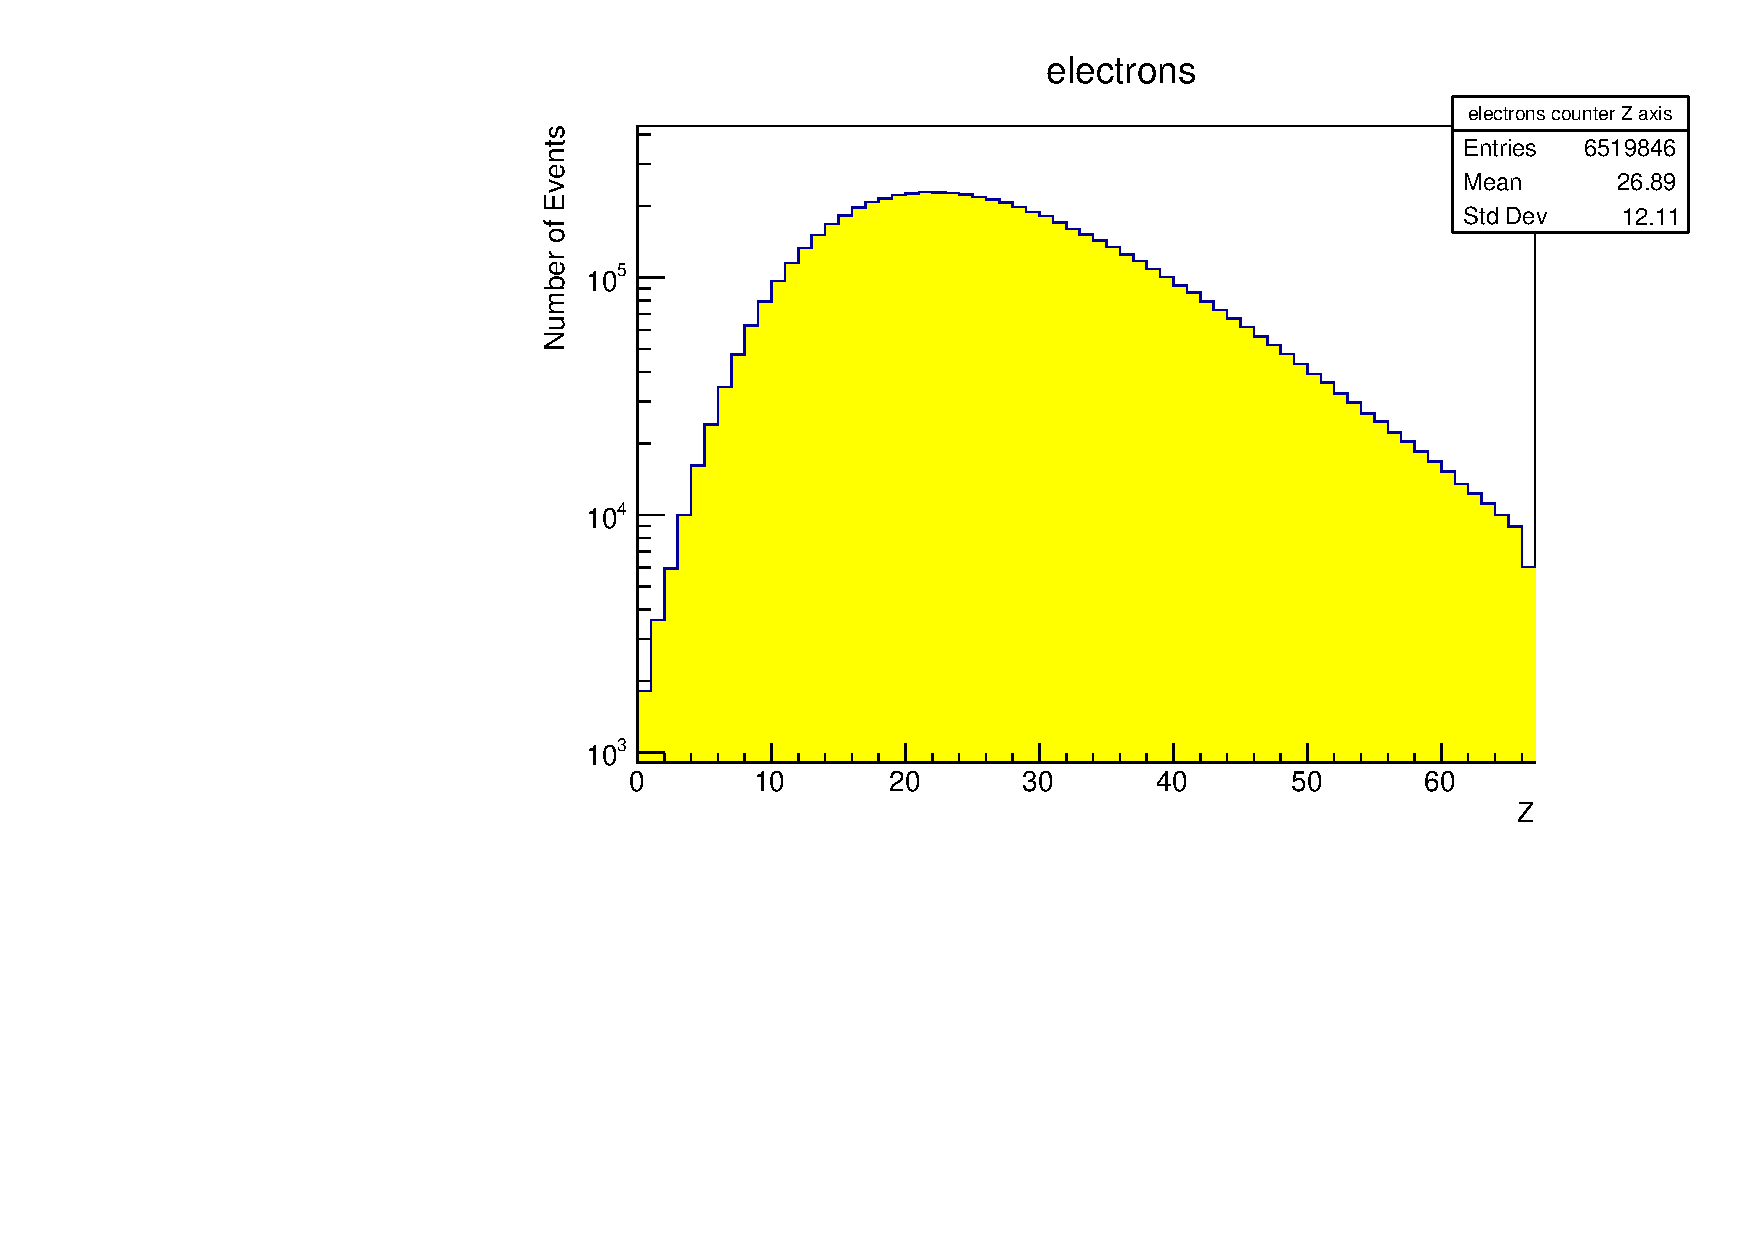
\includegraphics[scale=0.35]{Kap3/pi0_scintillator_electrons_plots_calo_counter_Z.pdf}\label{fig:electrons-creation-scintillator-6}}

  \caption{Electron creation in the scintillator plates of the calorimeter.}\label{fig:electrons-creation-scintillator}

\end{figure}

The same scenario can be seen for the created electrons in the scintillator
plates (see \cref{fig:electrons-creation-scintillator}). Again, the mean is in
the central plates, in this case, \((8.766, 5.696)\) for electrons, \((8.781,
5.704)\) for photons and \((8.746, 5.702)\) for the neutral pions. The pions
also have a wider vertical distribution with a standard deviation of \((3.430,
2.213)\), compared to the electrons, \((3.287, 1.855)\) and the photons,
\((3.283, 1.861)\).

\begin{figure}[htb!]
  \centering

  \subfloat[\(e^-\) as primary particle, X-Y plane of the calorimeter.]{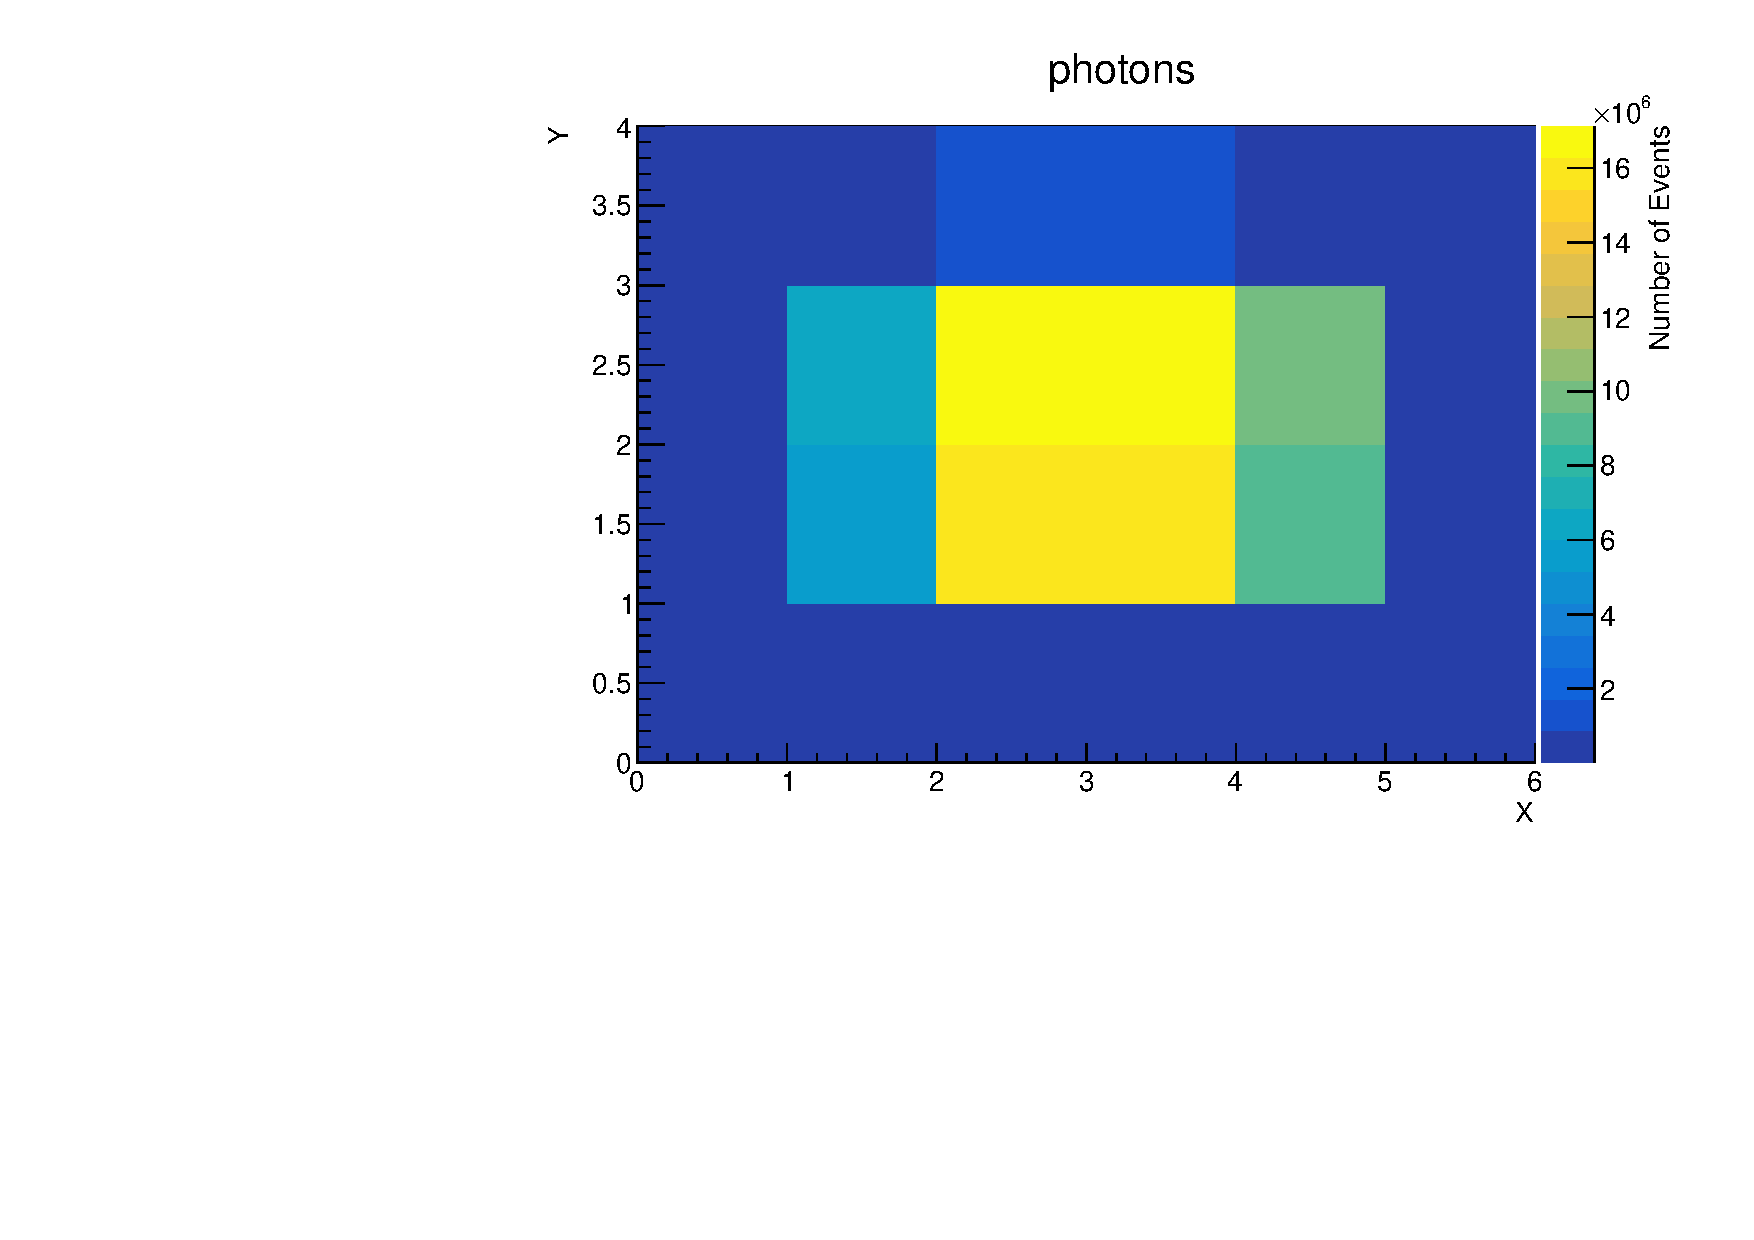
\includegraphics[scale=0.35]{Kap3/electron_lead_photons_plots_calo_counter.pdf}\label{fig:photons-creation-lead-1}}\hspace{1em}
  \subfloat[\(e^-\) as primary particle, Z axis of the calorimeter.]{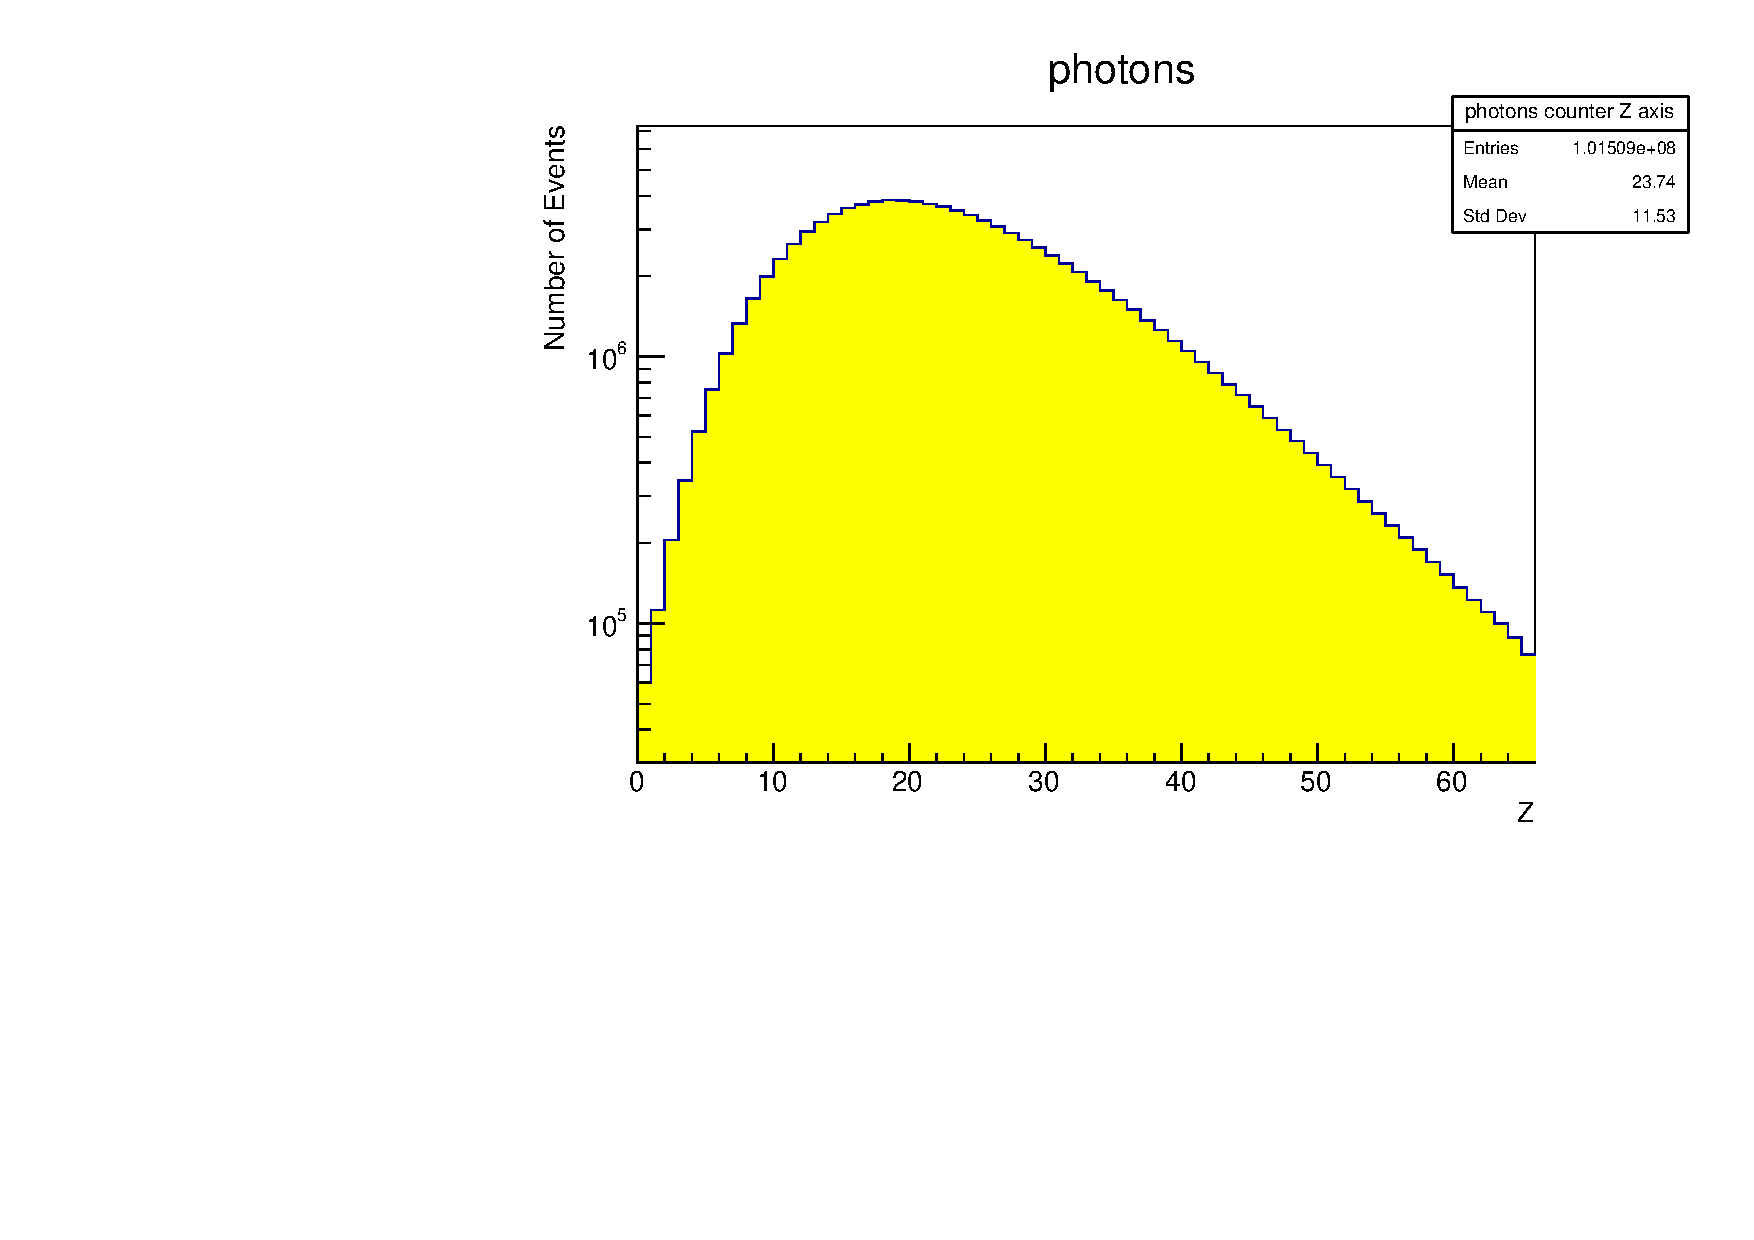
\includegraphics[scale=0.35]{Kap3/electron_lead_photons_plots_calo_counter_Z.pdf}\label{fig:photons-creation-lead-2}}

  \subfloat[\(\gamma\) as primary particle, X-Y plane of the calorimeter.]{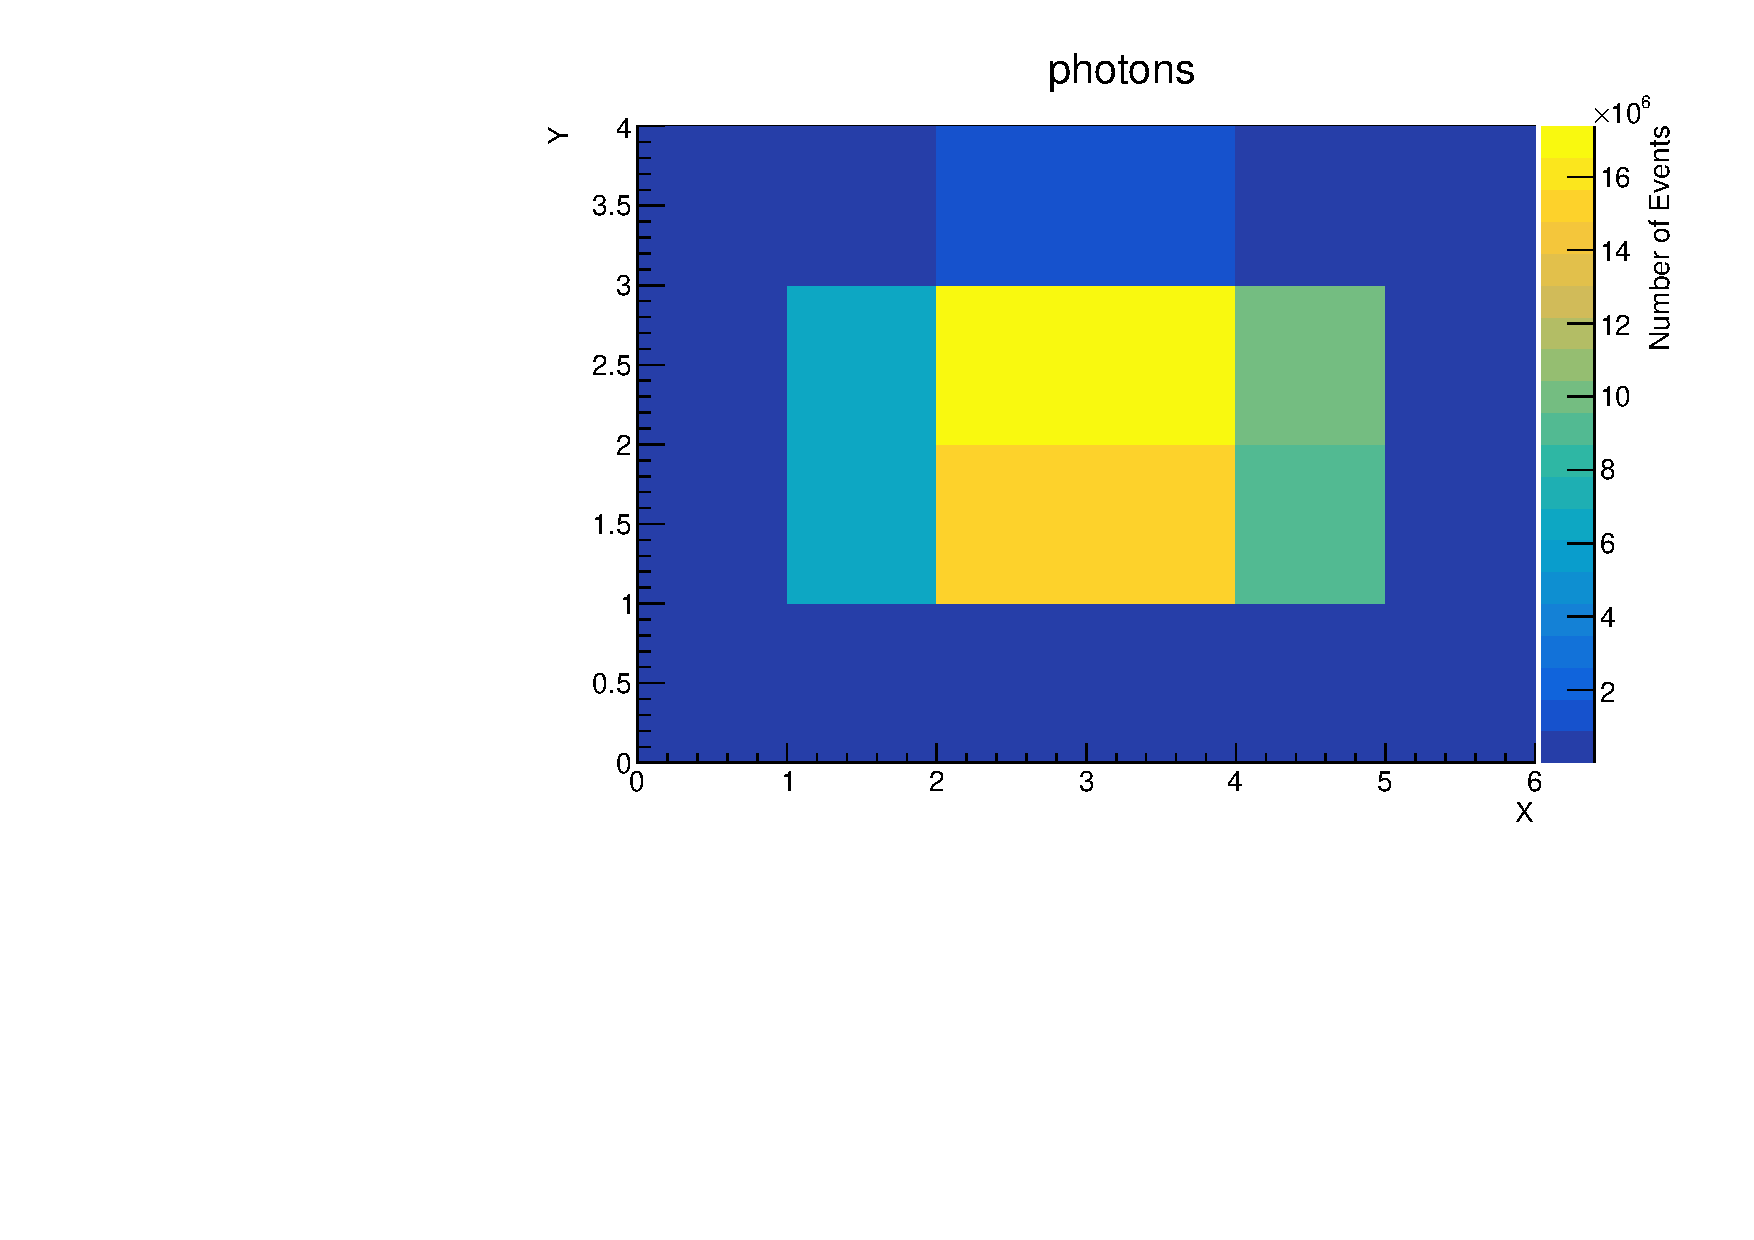
\includegraphics[scale=0.35]{Kap3/gamma_lead_photons_plots_calo_counter.pdf}\label{fig:photons-creation-lead-3}}\hspace{1em}
  \subfloat[\(\gamma\) as primary particle, Z axis of the calorimeter.]{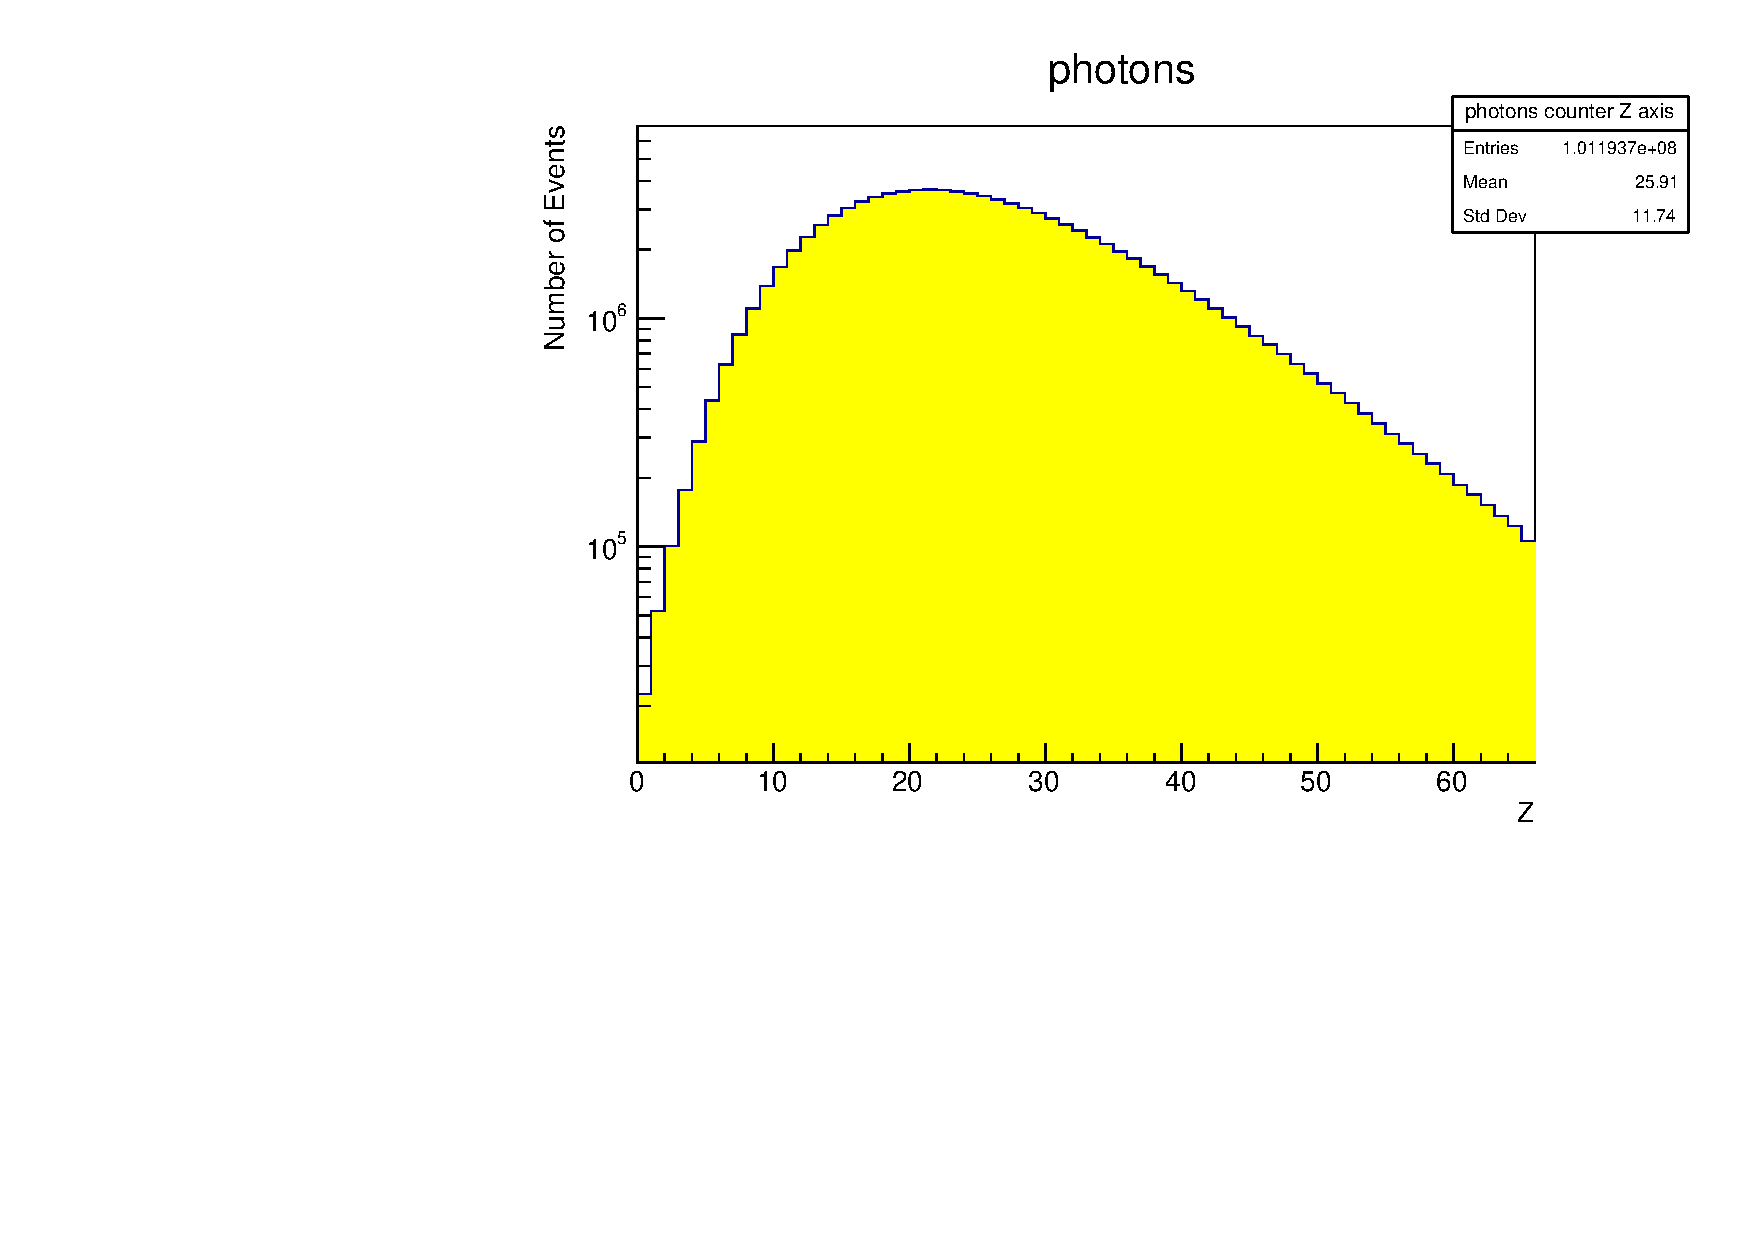
\includegraphics[scale=0.35]{Kap3/gamma_lead_photons_plots_calo_counter_Z.pdf}\label{fig:photons-creation-lead-4}}

  \subfloat[\(\pi^0\) as primary particle, X-Y plane of the calorimeter.]{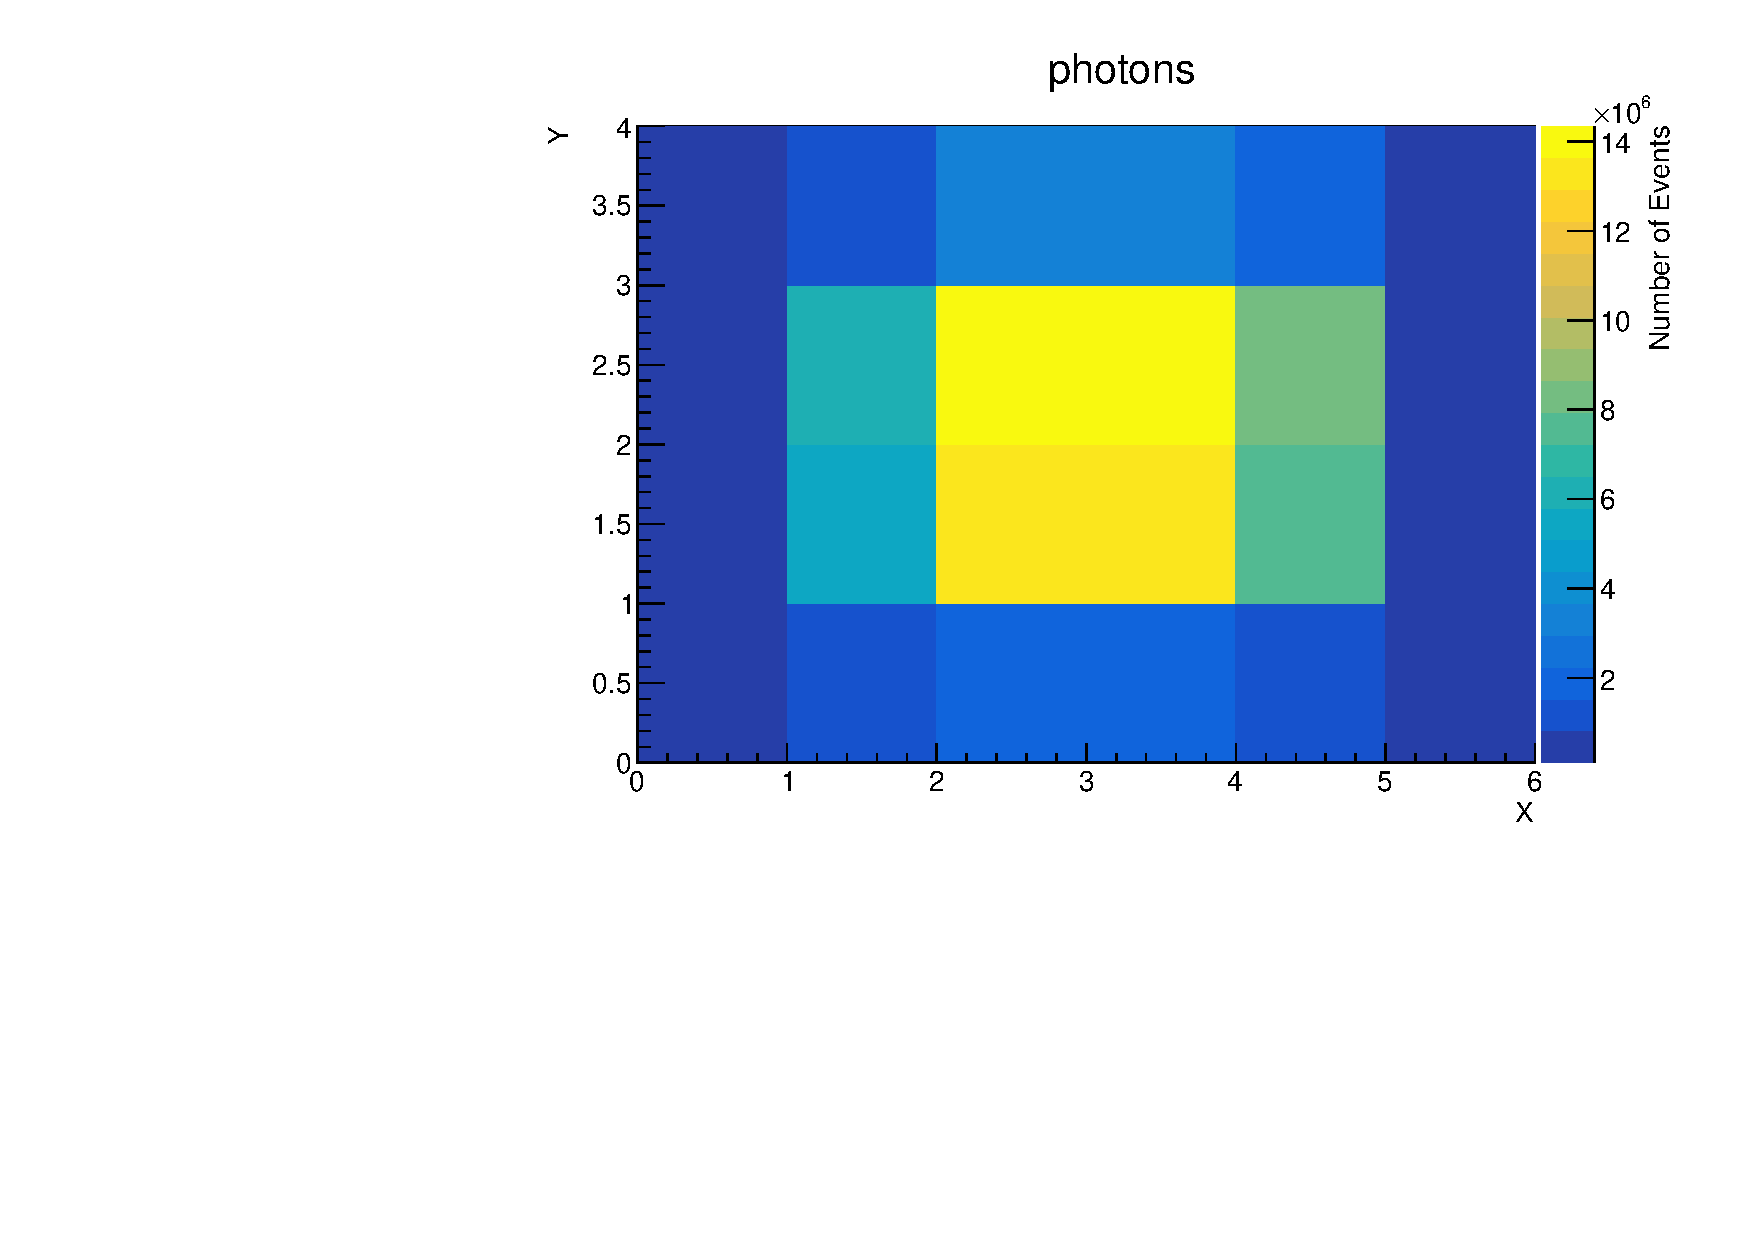
\includegraphics[scale=0.35]{Kap3/pi0_lead_photons_plots_calo_counter.pdf}\label{fig:photons-creation-lead-5}}\hspace{1em}
  \subfloat[\(\pi^0\) as primary particle, Z axis of the calorimeter.]{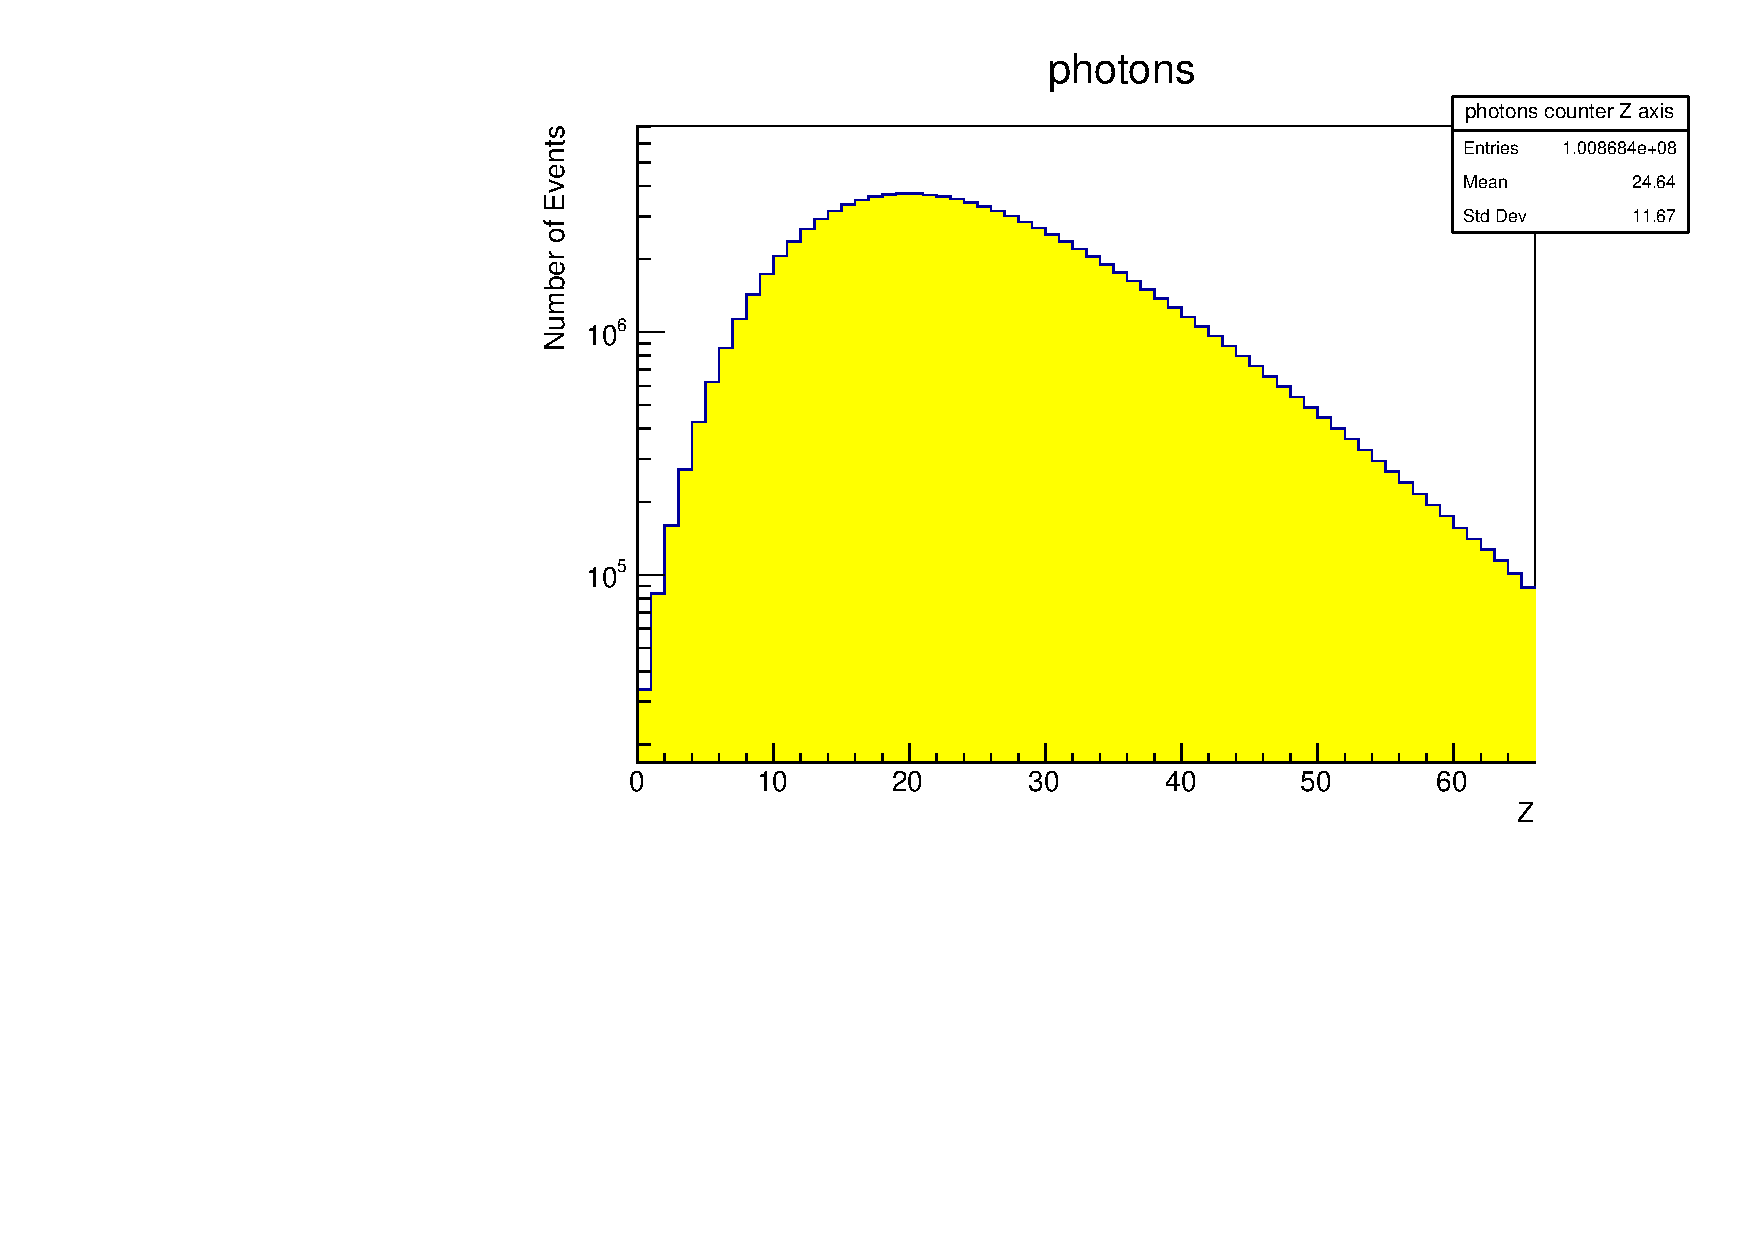
\includegraphics[scale=0.35]{Kap3/pi0_lead_photons_plots_calo_counter_Z.pdf}\label{fig:photons-creation-lead-6}}

  \caption{Photons creation in the lead plates of the calorimeter.}\label{fig:photons-creation-lead}

\end{figure}

For both electron and protons, the distribution in the Z axis did not show
significant differences, the mean values are very close one from each other,
however it is to mention that in the two cases, the lowest mean value is when
the primary particle is an electron, and the greatest when it is a photon.

In the case of the particle production in the lead, the main value is again in
the central zone of the detector, and also, the standard deviations in the
pions signal is larger. For the photon creation, shown in the
\cref{fig:photons-creation-lead}, the standard deviation of the electrons,
photons and pions are \((0.949, 0.584)\), \((0.951, 0.583)\) and \((1.028,
0.758)\) respectively.

\begin{figure}[htb!]
  \centering

  \subfloat[\(e^-\) as primary particle, X-Y plane of the calorimeter.]{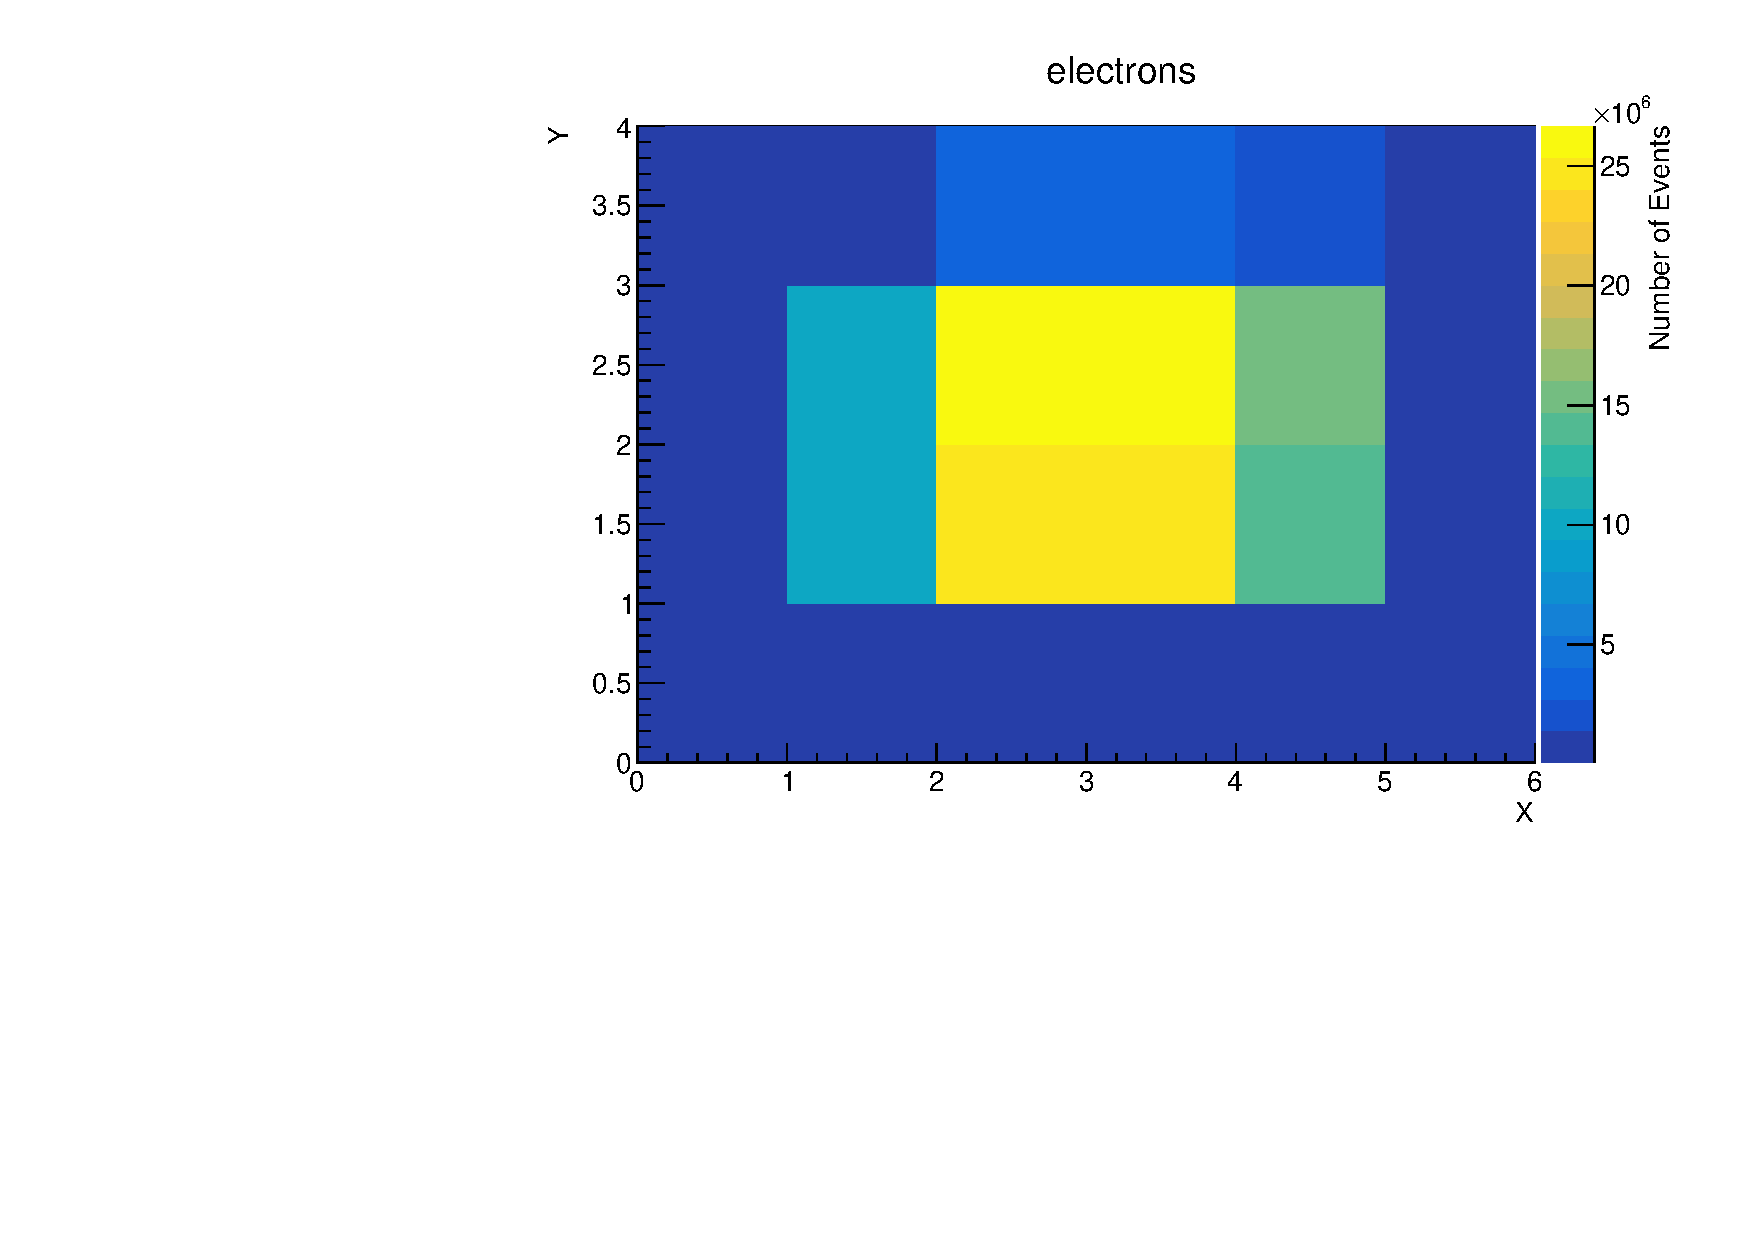
\includegraphics[scale=0.35]{Kap3/electron_lead_electrons_plots_calo_counter.pdf}\label{fig:electrons-creation-lead-1}}\hspace{1em}
  \subfloat[\(e^-\) as primary particle, Z axis of the calorimeter.]{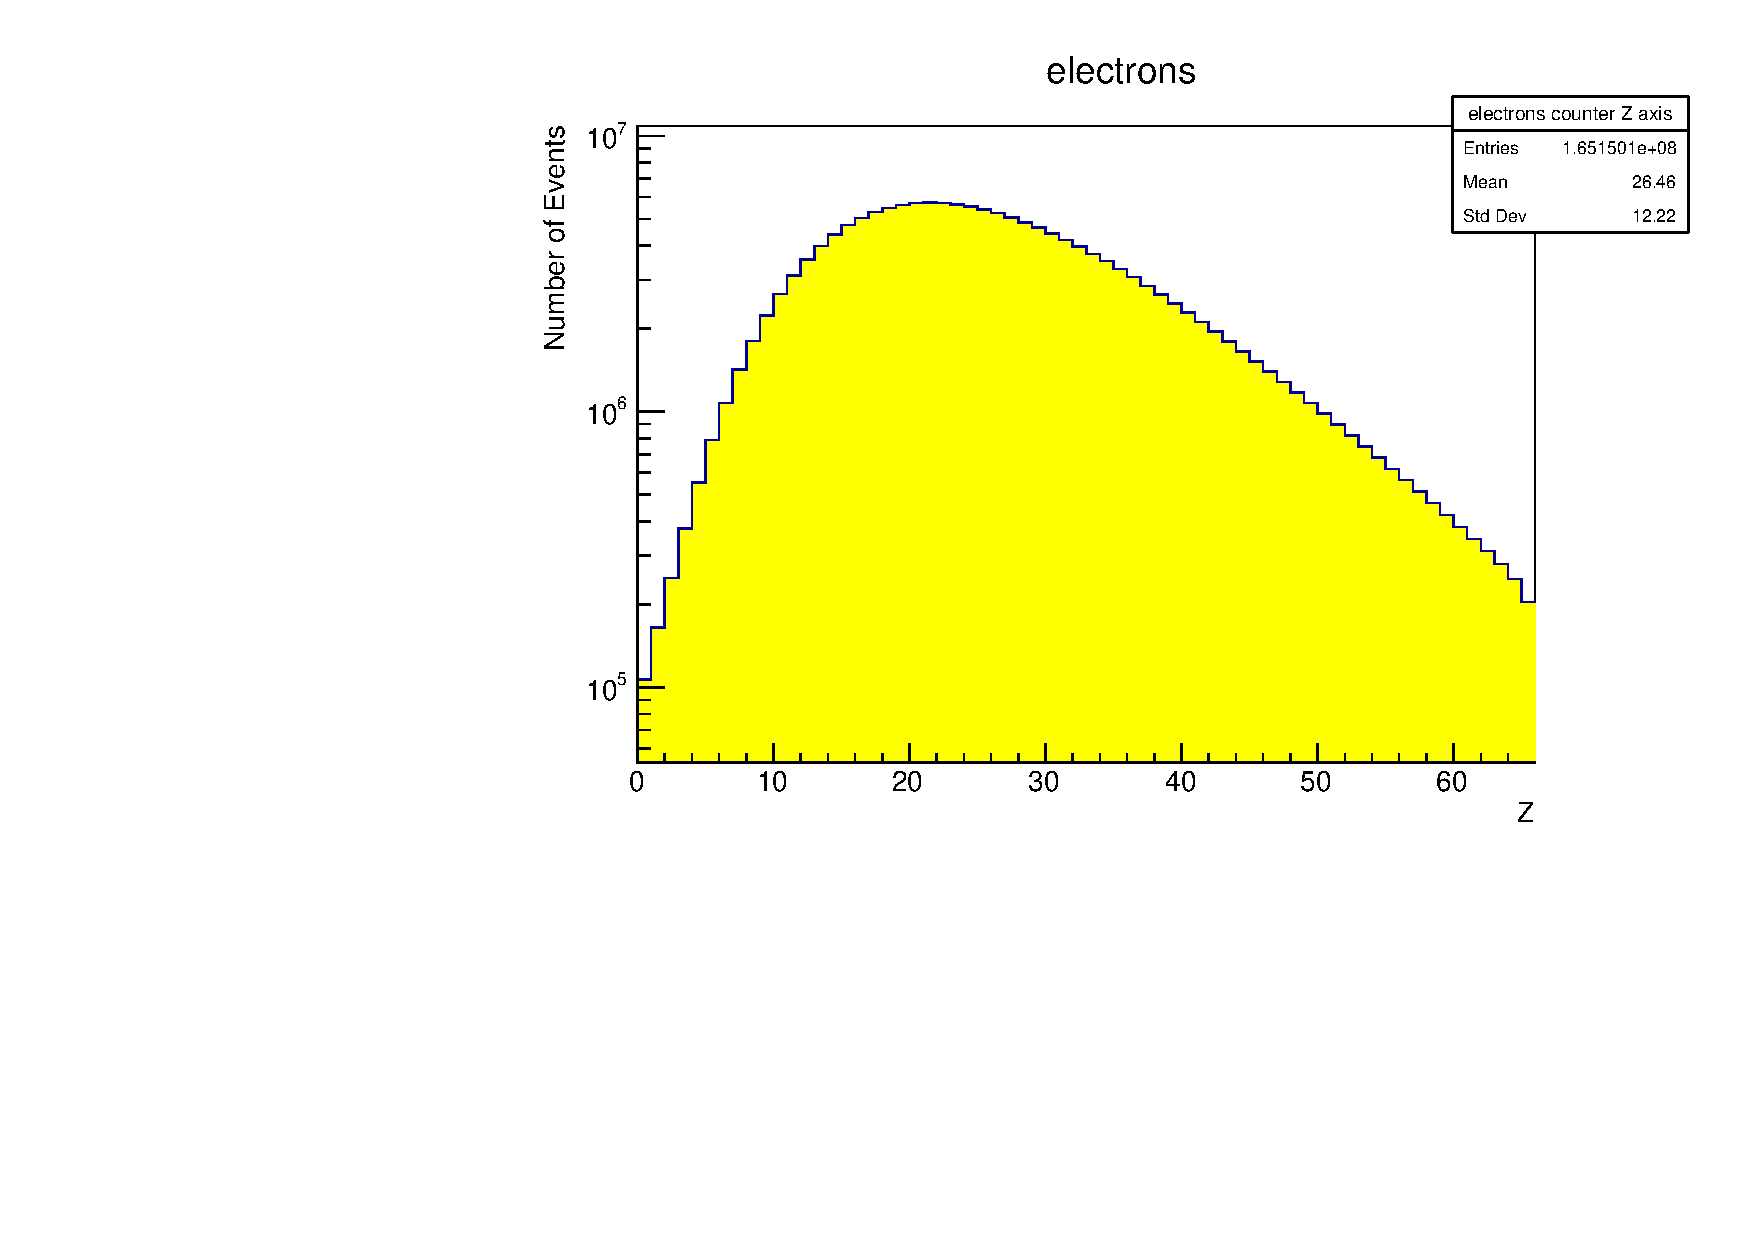
\includegraphics[scale=0.35]{Kap3/electron_lead_electrons_plots_calo_counter_Z.pdf}\label{fig:electrons-creation-lead-2}}

  \subfloat[\(\gamma\) as primary particle, X-Y plane of the calorimeter.]{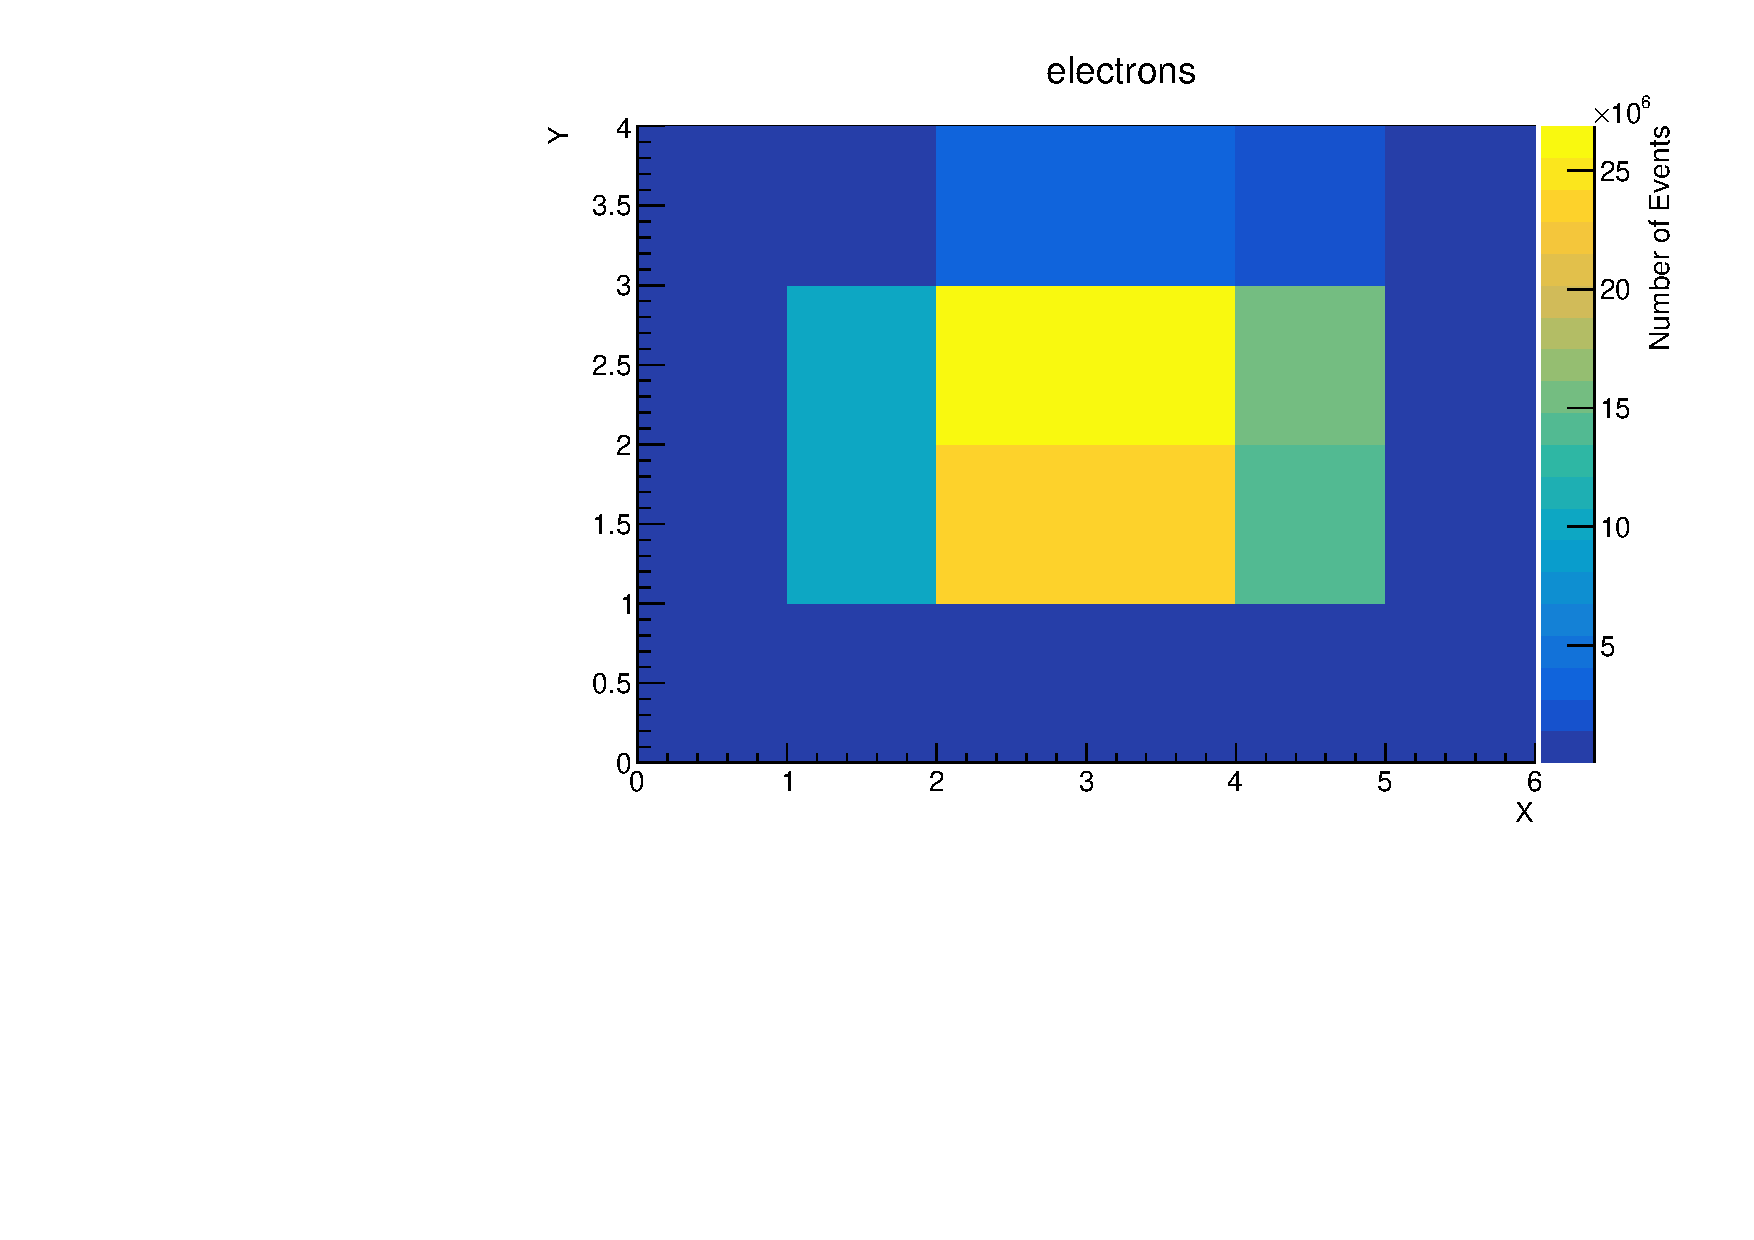
\includegraphics[scale=0.35]{Kap3/gamma_lead_electrons_plots_calo_counter.pdf}\label{fig:electrons-creation-lead-3}}\hspace{1em}
  \subfloat[\(\gamma\) as primary particle, Z axis of the calorimeter.]{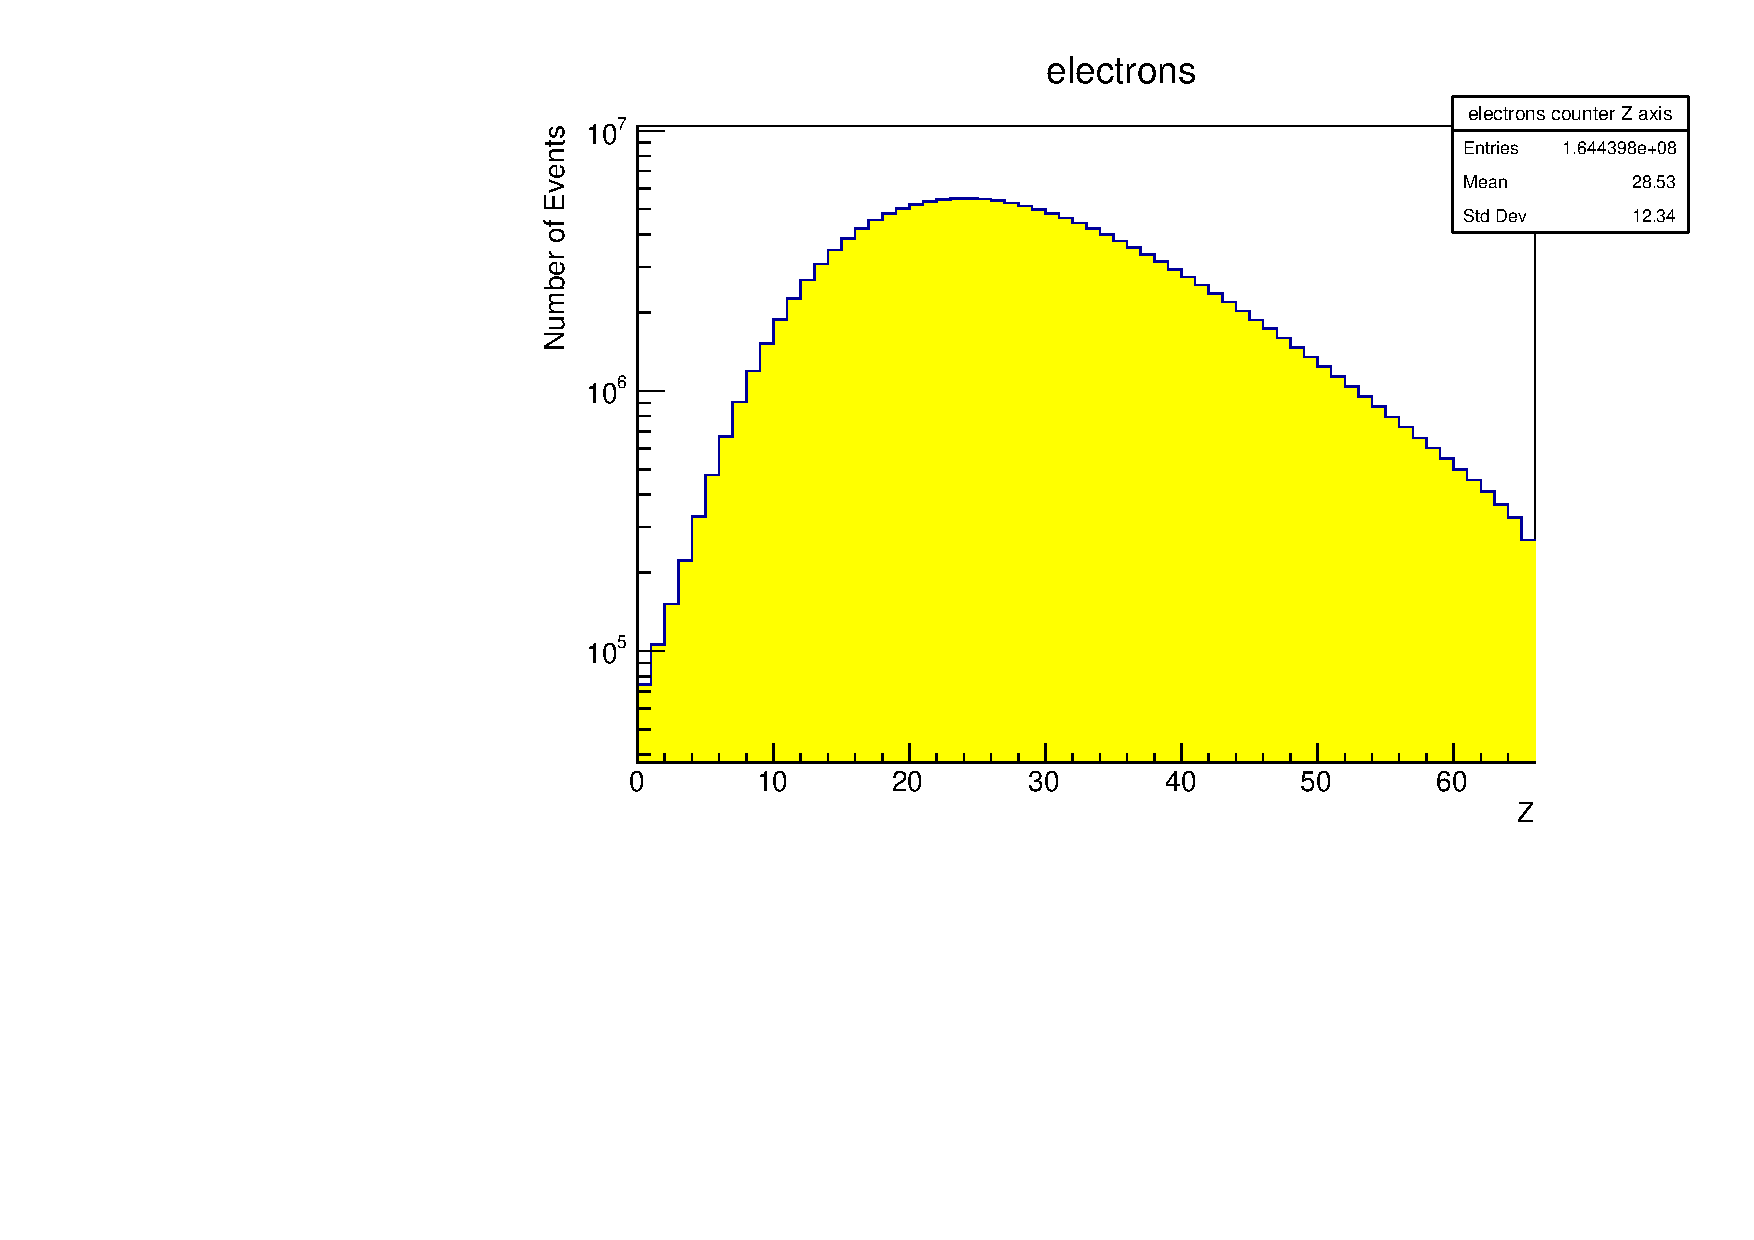
\includegraphics[scale=0.35]{Kap3/gamma_lead_electrons_plots_calo_counter_Z.pdf}\label{fig:electrons-creation-lead-4}}

  \subfloat[\(\pi^0\) as primary particle, X-Y plane of the calorimeter.]{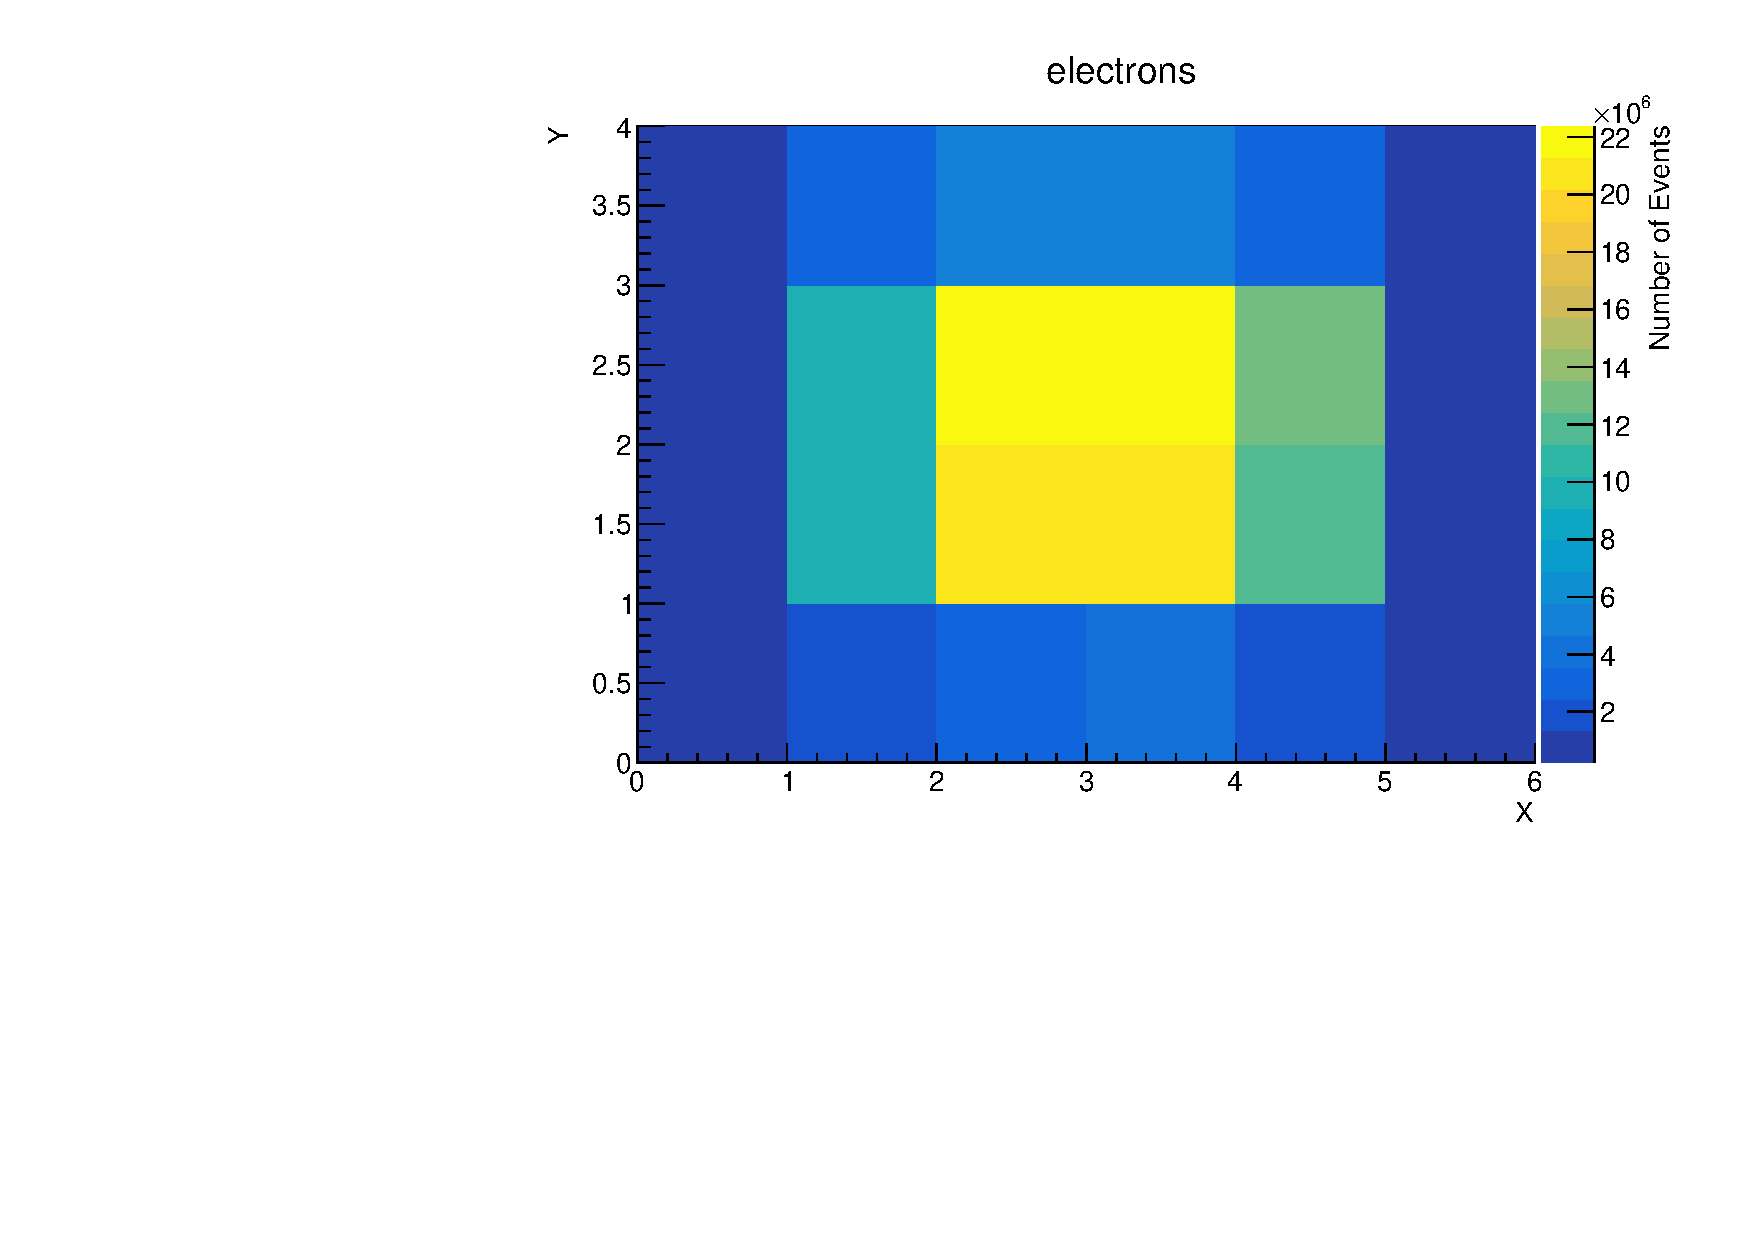
\includegraphics[scale=0.35]{Kap3/pi0_lead_electrons_plots_calo_counter.pdf}\label{fig:electrons-creation-lead-5}}\hspace{1em}
  \subfloat[\(\pi^0\) as primary particle, Z axis of the calorimeter.]{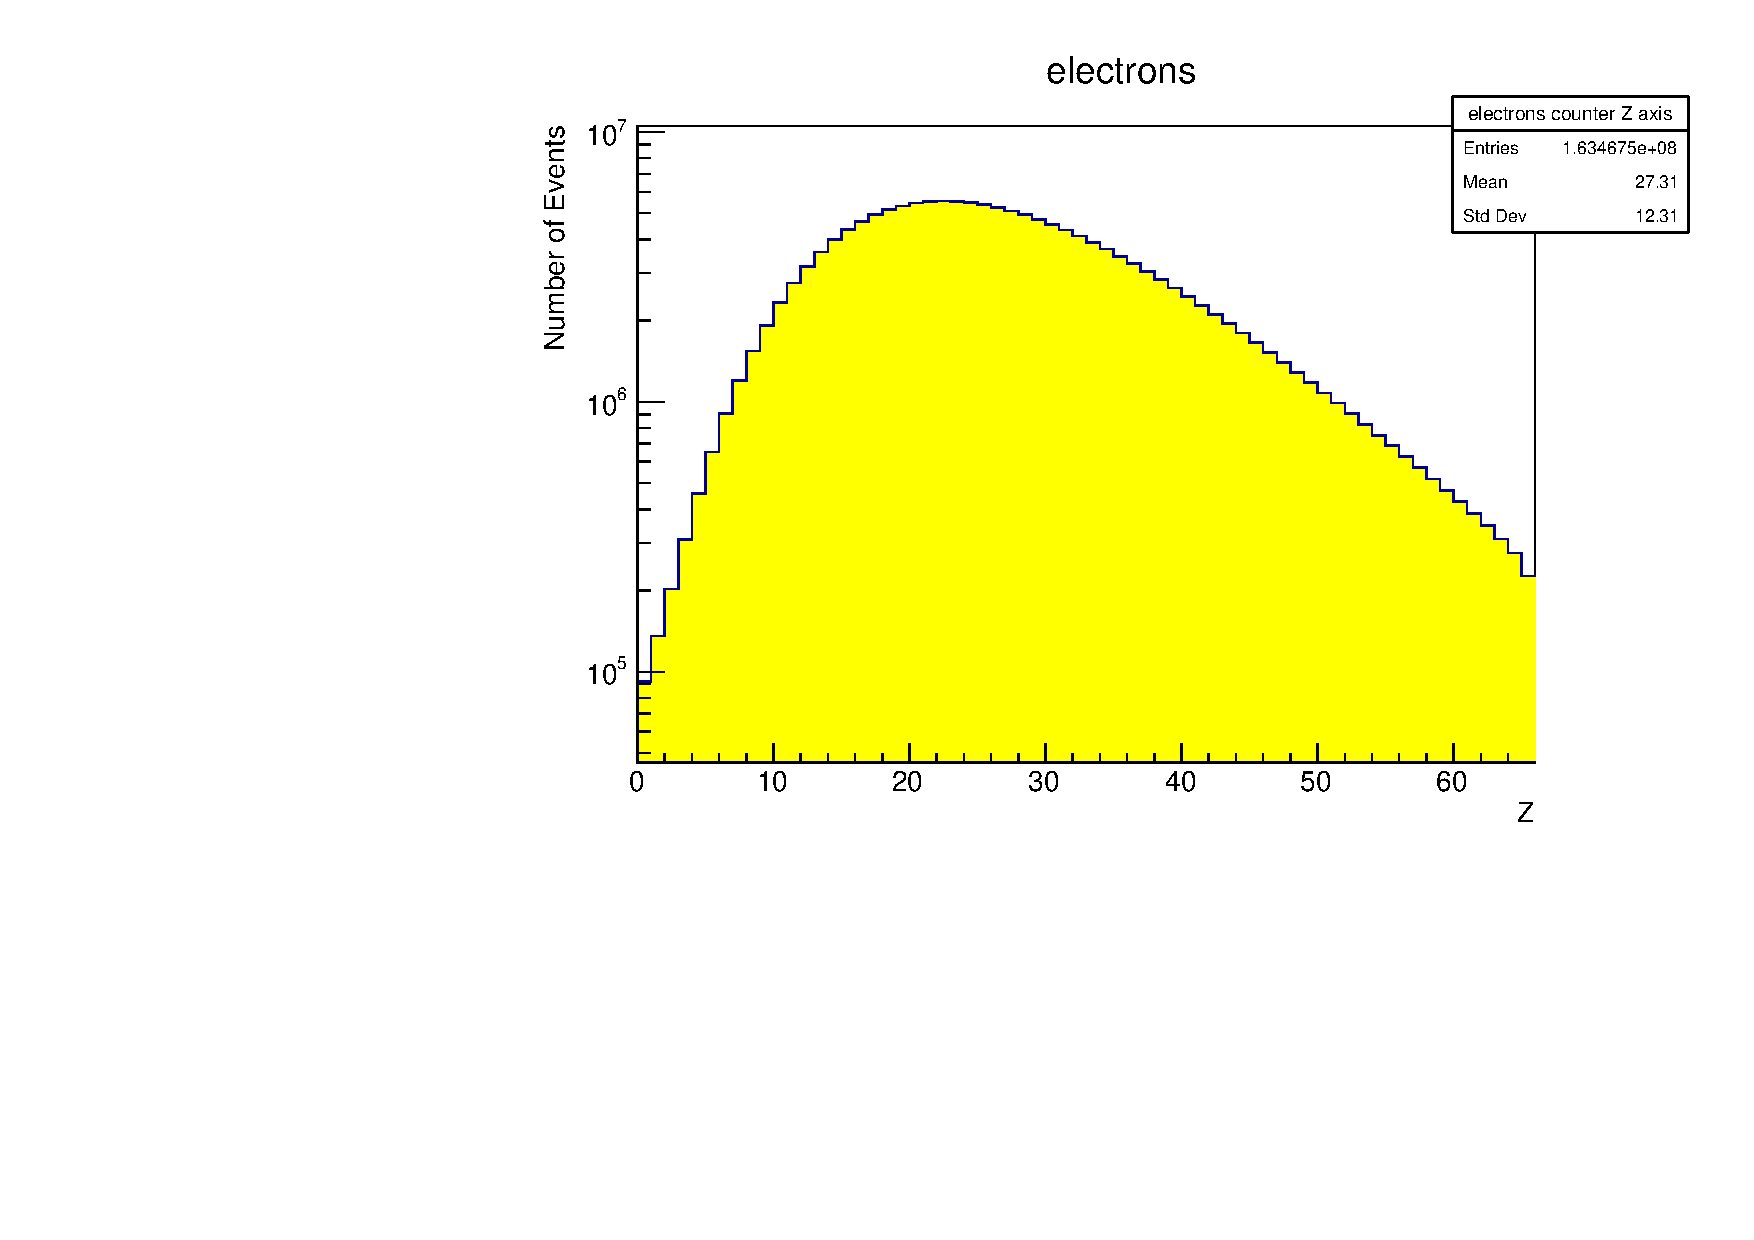
\includegraphics[scale=0.35]{Kap3/pi0_lead_electrons_plots_calo_counter_Z.pdf}\label{fig:electrons-creation-lead-6}}


  \caption{Electron creation in the lead plates of the calorimeter.}\label{fig:electrons-creation-lead}


\end{figure}

For the electron creation as illustrated in \cref{fig:electrons-creation-lead},
the standard deviation for electrons, photons and pions are \((0.9663,
0.6340)\), \((0.9668, 0.6346)\) and \((1.047, 0.7789)\) respectively. Again,
the standard deviation for the neutral pions if large.

\begin{figure}[htb!]
  \centering

  \subfloat[\(e^-\) as primary particle.]{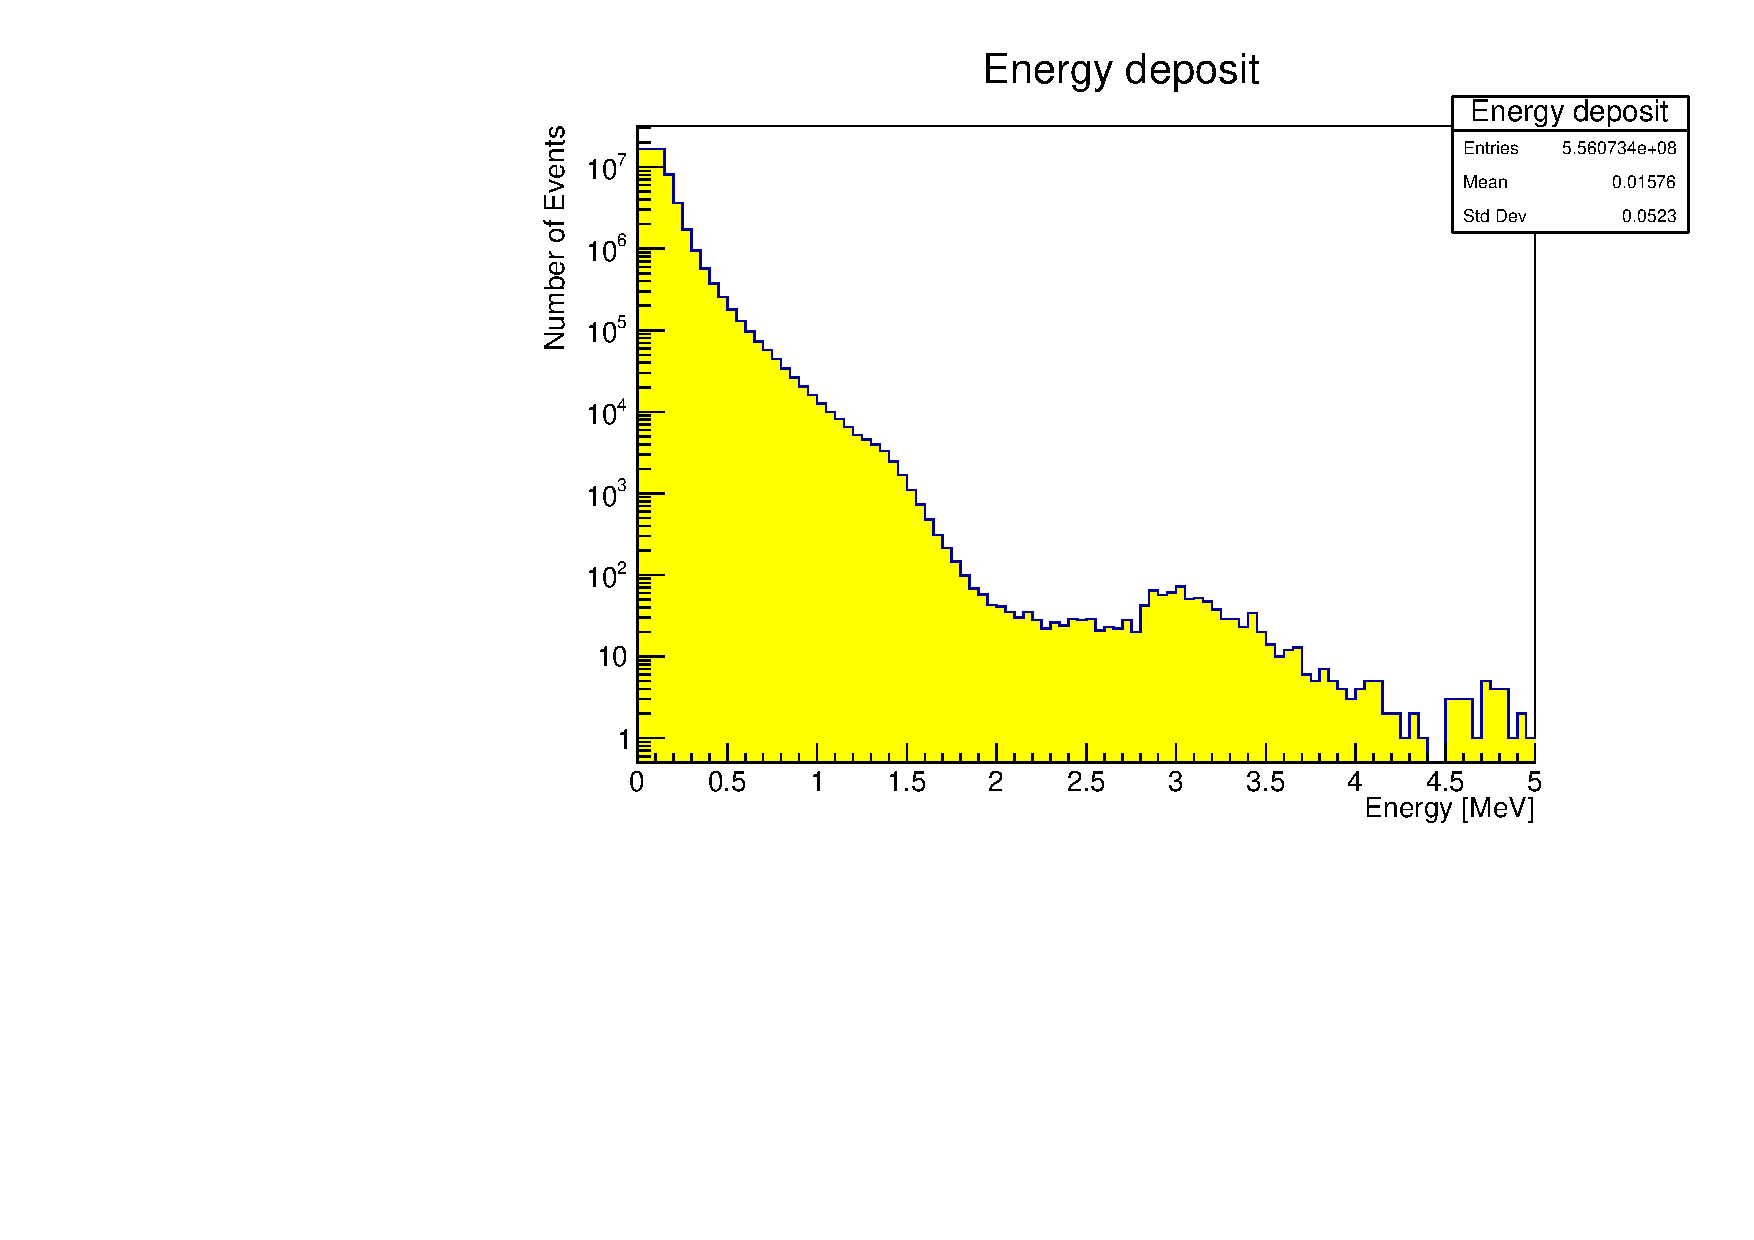
\includegraphics[scale=0.35]{Kap3/electron_scintillator_electrons_plots_energy_hist.pdf}\label{fig:energy-scintillator-1}}\hspace{1em}
  \subfloat[\(\gamma\) as primary particle.]{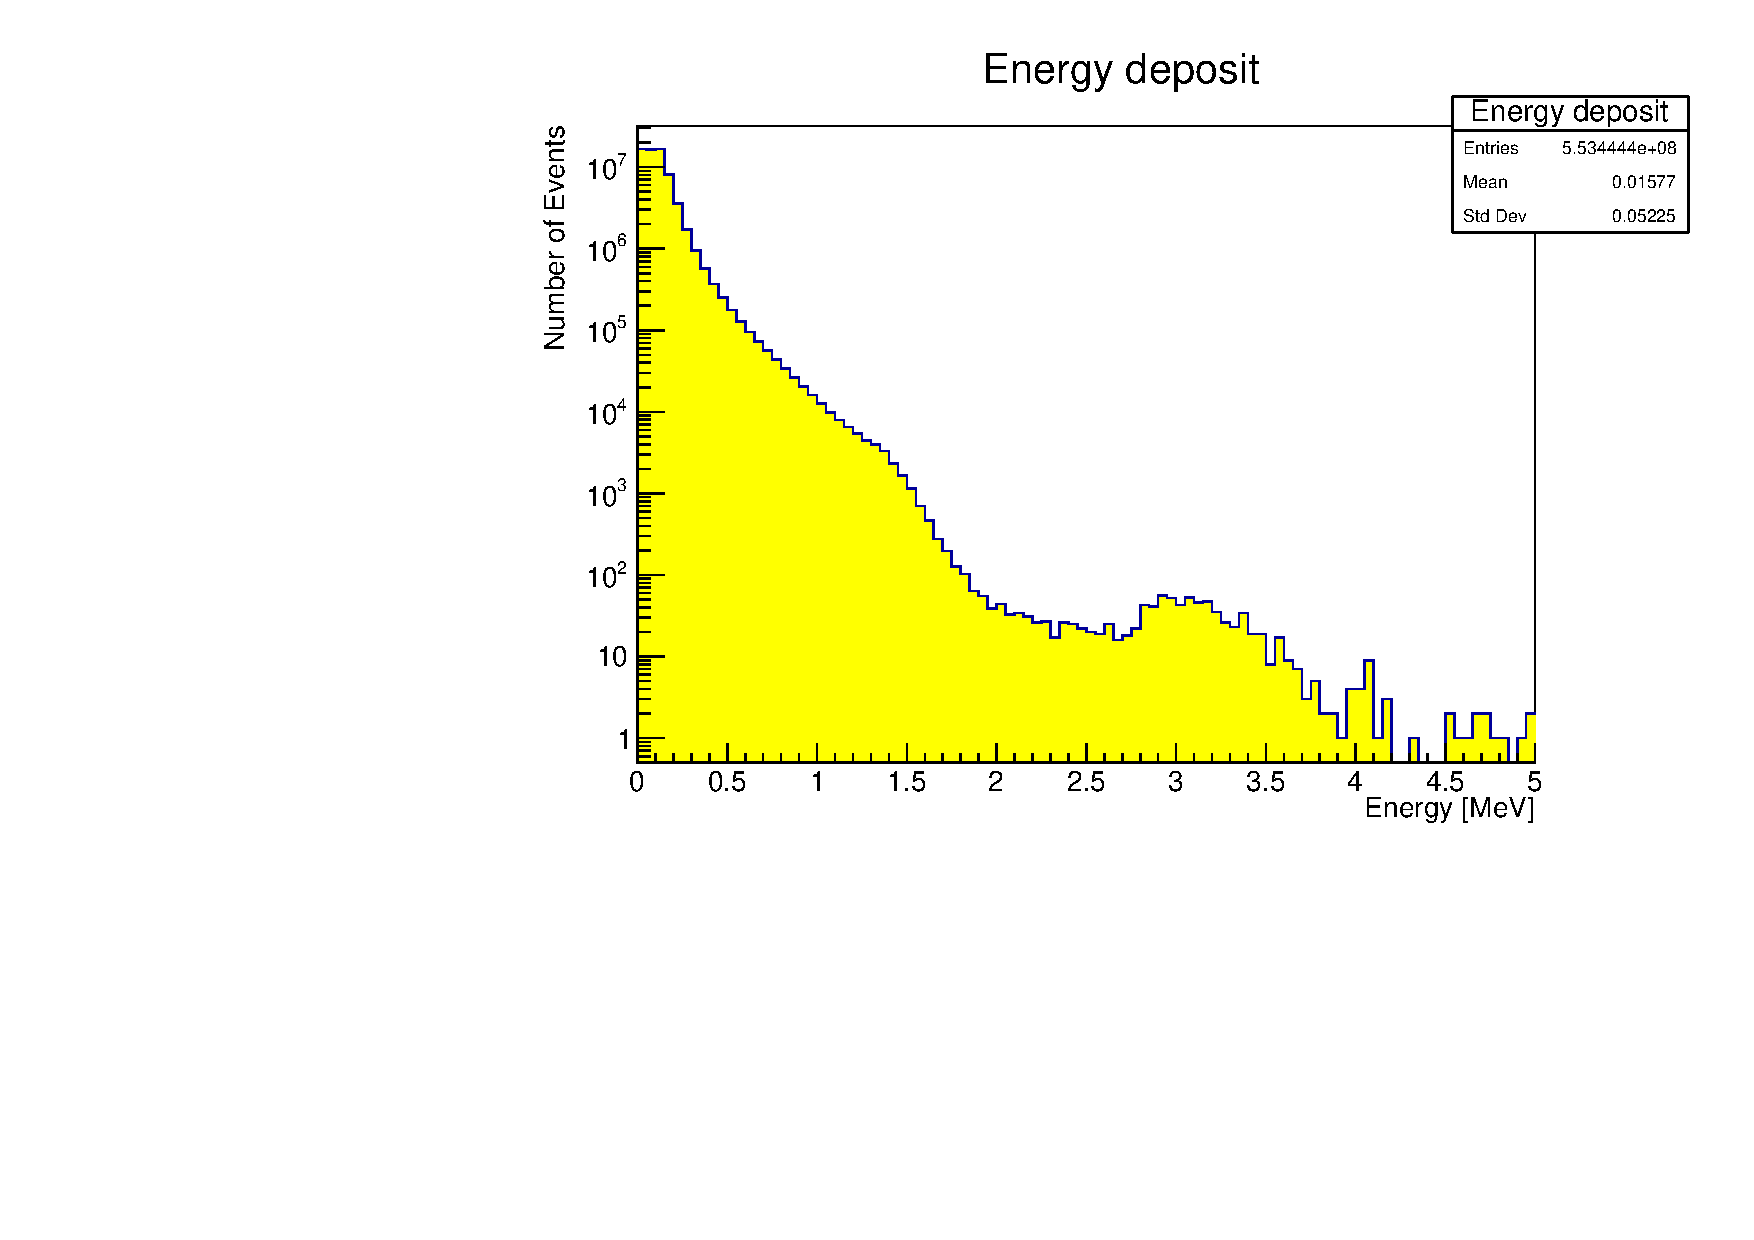
\includegraphics[scale=0.35]{Kap3/gamma_scintillator_electrons_plots_energy_hist.pdf}\label{fig:energy-scintillator-2}}\hspace{1em}
  \subfloat[\(\pi^0\) as primary particle.]{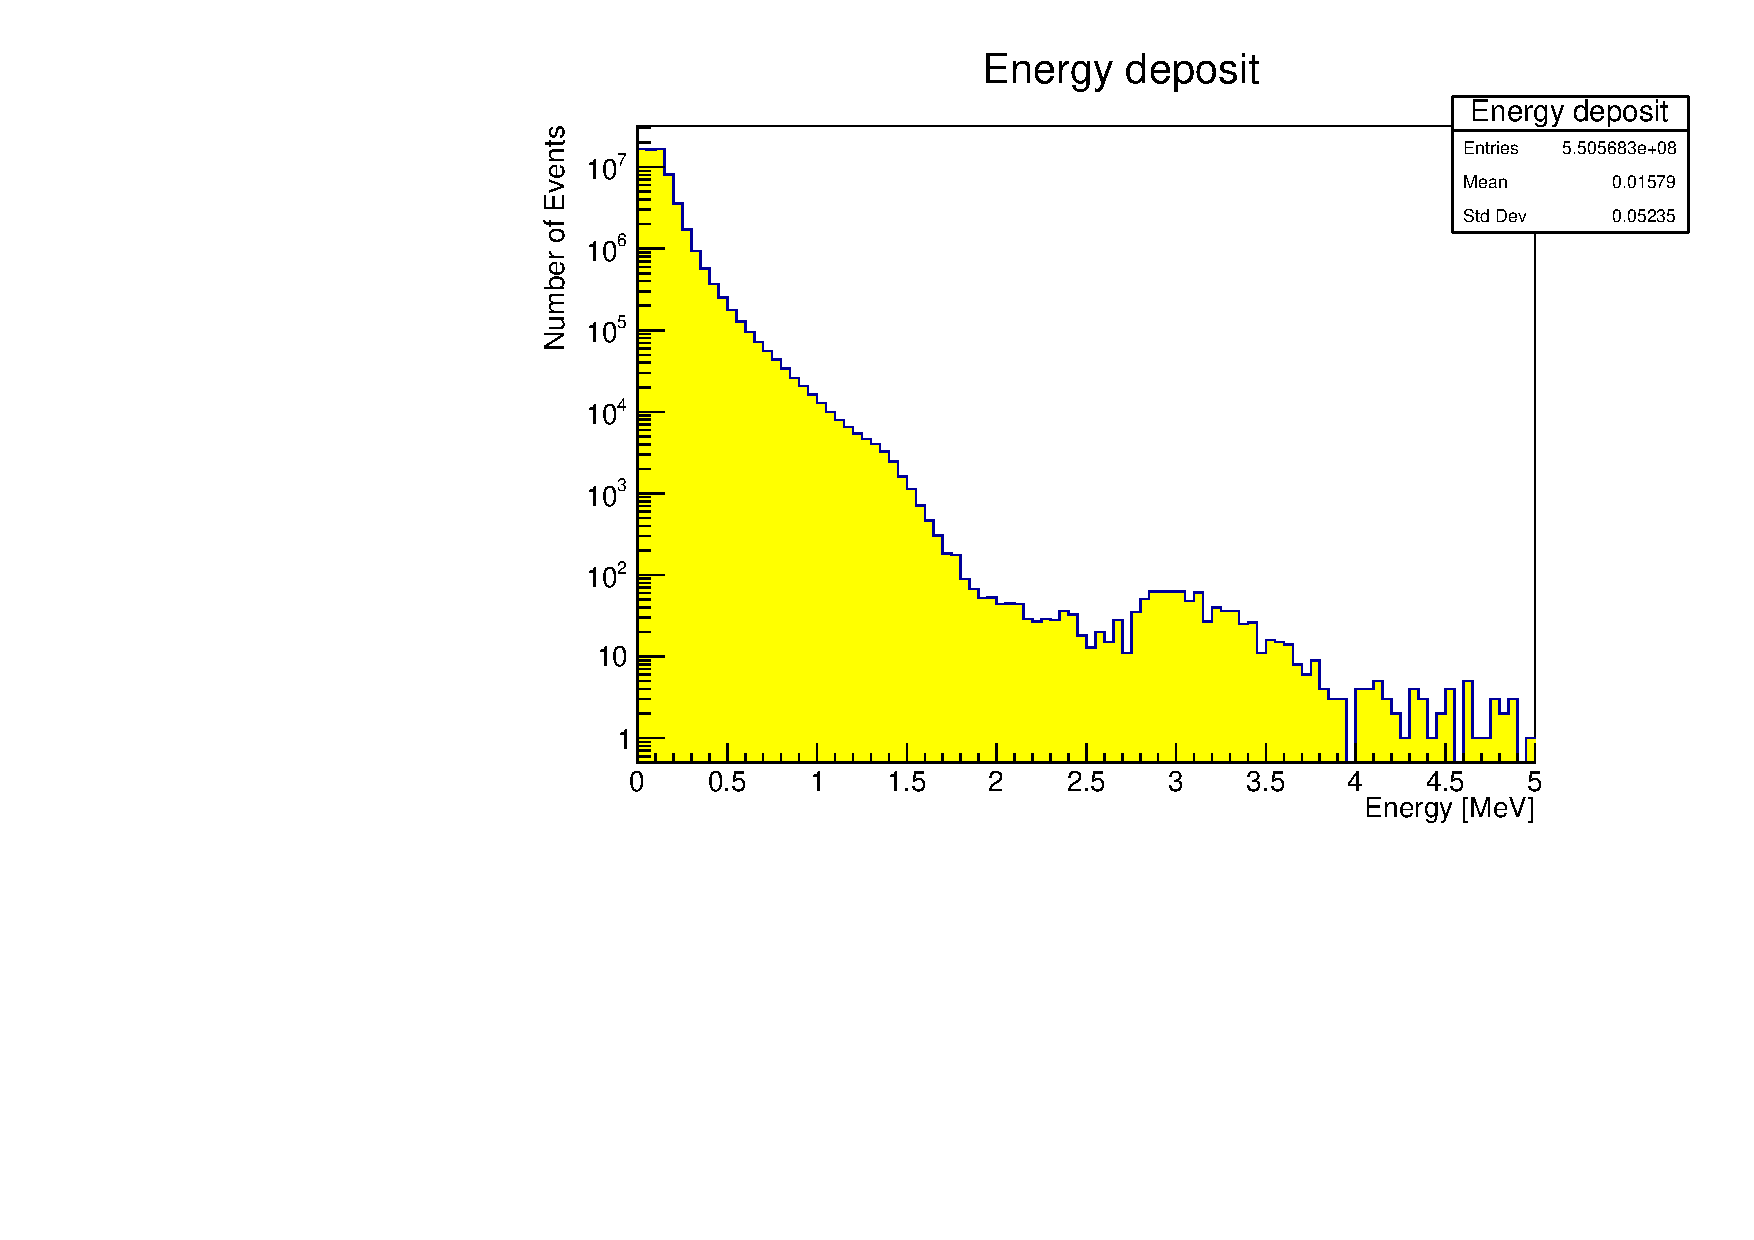
\includegraphics[scale=0.35]{Kap3/pi0_scintillator_electrons_plots_energy_hist.pdf}\label{fig:energy-scintillator-3}}

  \caption{Energy deposit in the scintillator plates of the calorimeter.}\label{fig:energy-scintillator}

\end{figure}

Again, the both cases do not show considerable differences in the particle
distribution along the Z axis, with the only particularity that the electrons
as primary particles have the lowest mean, and the photons the greatest.

It is important to mention that against expected, the average amount of
particles created per event is greater in lead than in the scintillator, the
mean number of photons created in the scintillator is \(261.97\), \(261.119\)
and \(260.267\) when the primary particle is an electron, a photon and a
neutral pion respectively, meanwhile for the lead the averages of photons
generated for the three primary particle are \(10150.9\), \(10119.4\) and
\(10086.8\). It means, in average in the lead the photons are produced almost
four times more than in the scintillator.

The electron production shows similar results, scintillator plates produce in
average \(658.594\), \(655.669\) and \(651.985\) electrons for electrons,
photons and neutral pions as primary particles respectively, but lead plates
produce \(16515\), \(16444\) and \(16346.8\), almost three times more. Note
also that the electron yield is greater than the photon yield for both
materials.

\begin{figure}[htb!]
  \centering

  \subfloat[\(e^-\) as primary particle.]{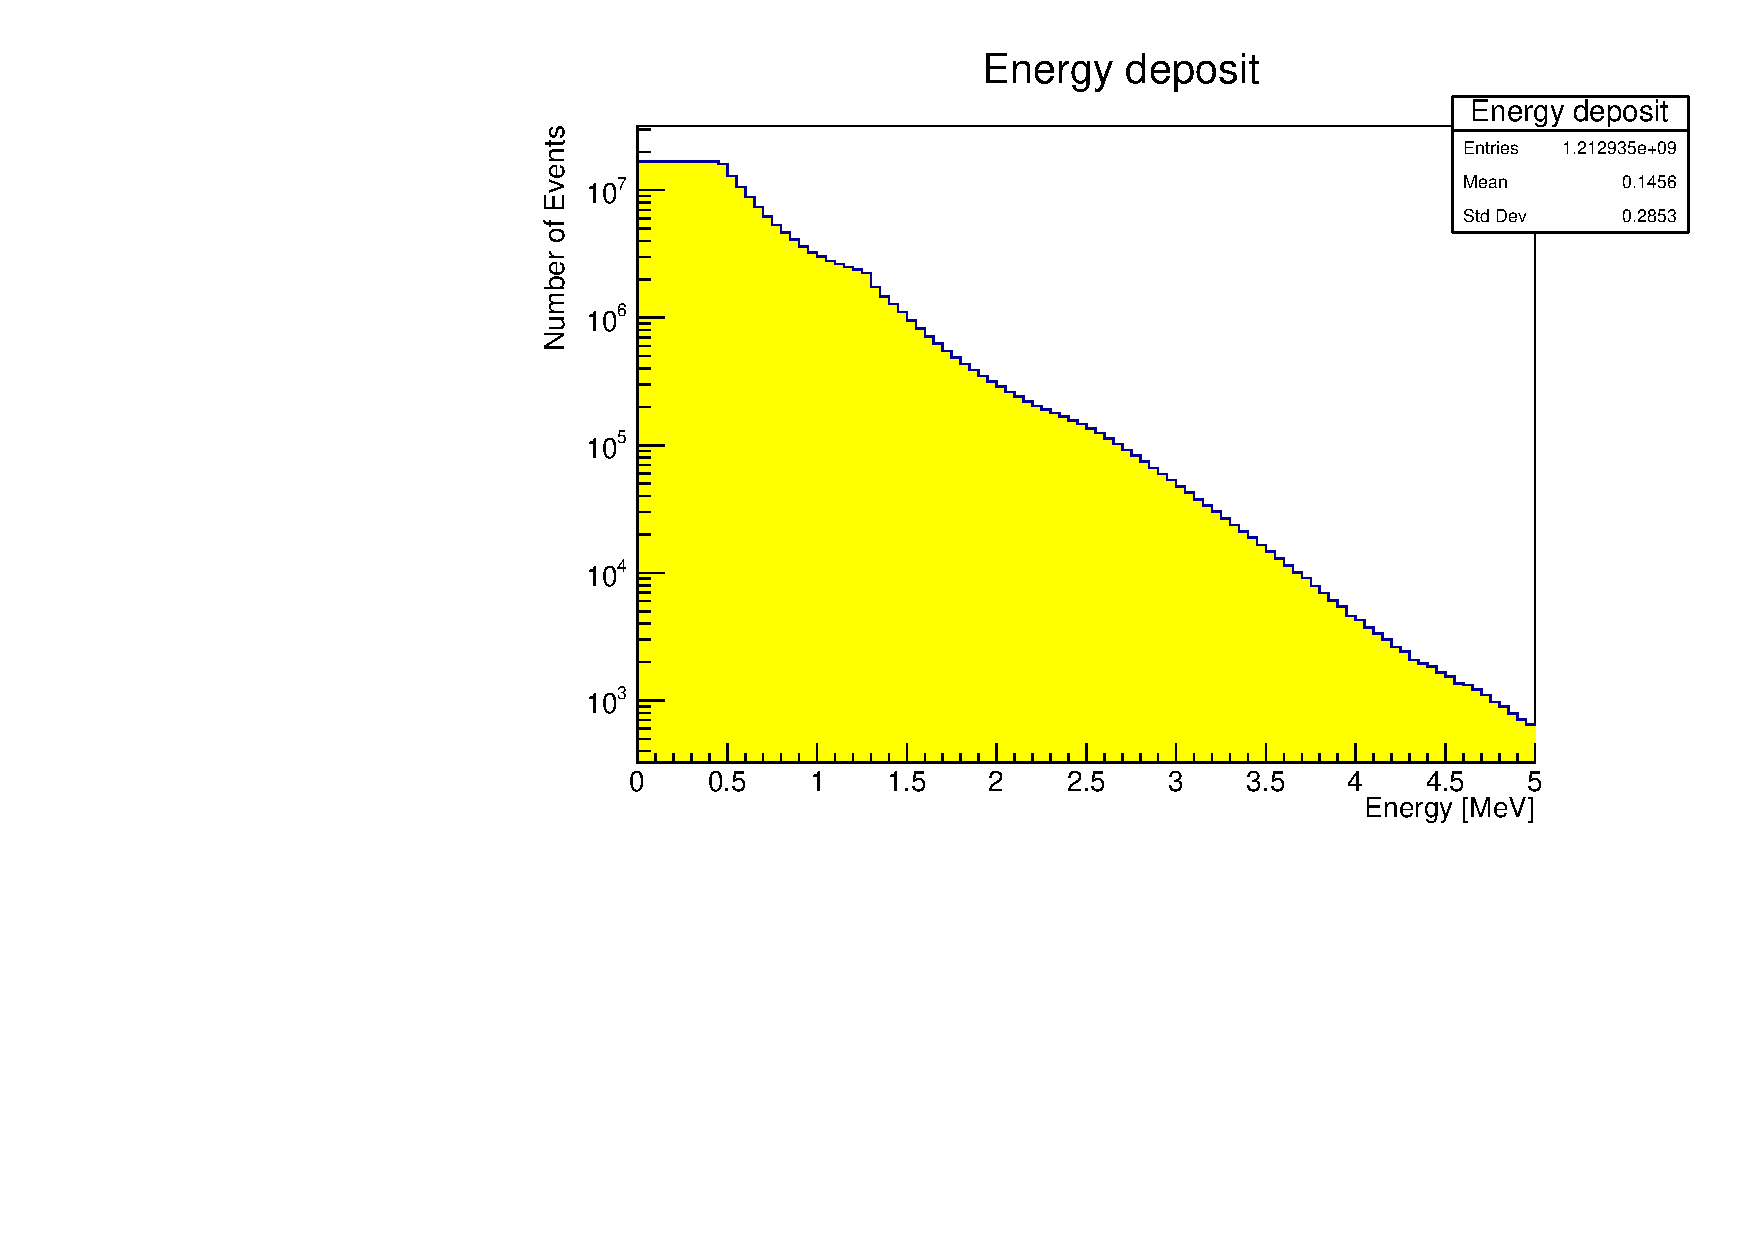
\includegraphics[scale=0.35]{Kap3/electron_lead_electrons_plots_energy_hist.pdf}\label{fig:energy-lead-1}}\hspace{1em}
  \subfloat[\(\gamma\) as primary particle.]{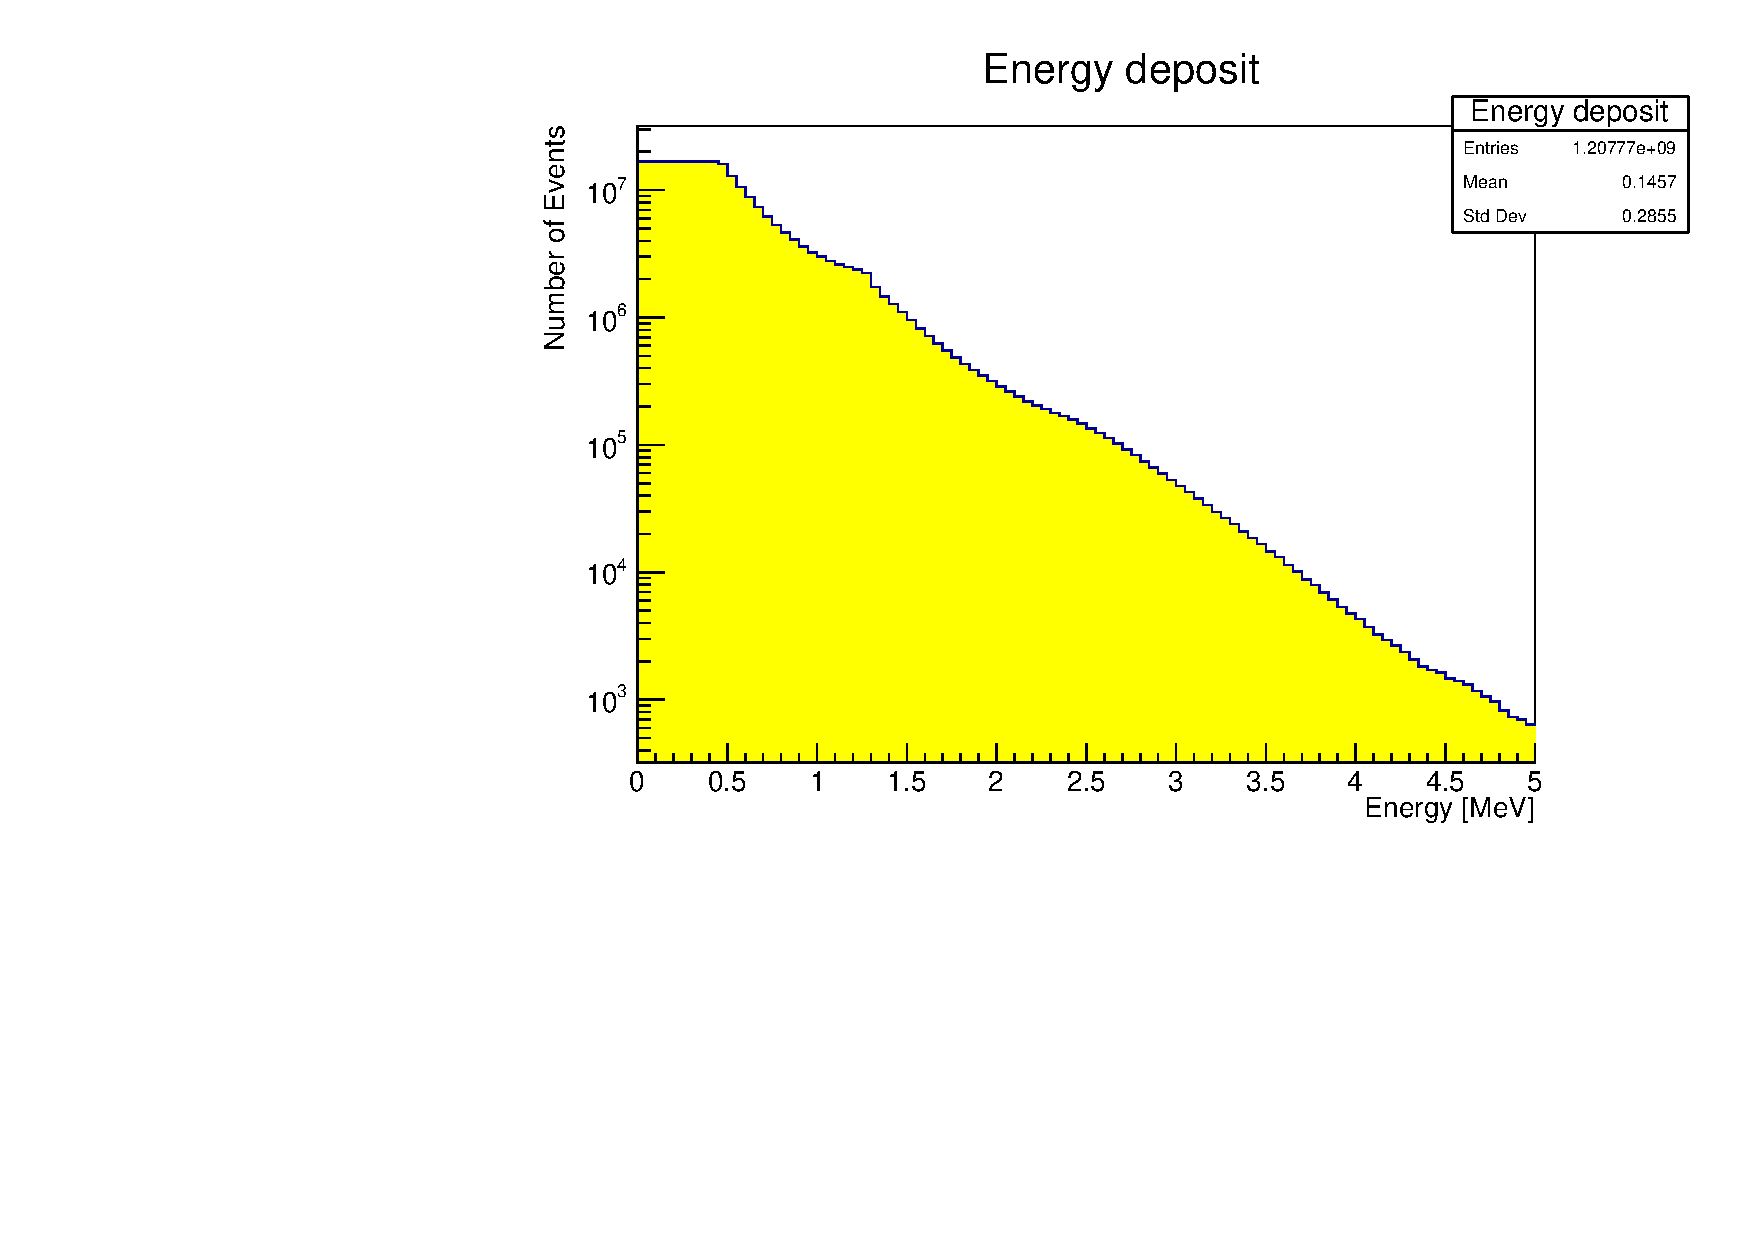
\includegraphics[scale=0.35]{Kap3/gamma_lead_electrons_plots_energy_hist.pdf}\label{fig:energy-lead-2}}\hspace{1em}
  \subfloat[\(\pi^0\) as primary particle.]{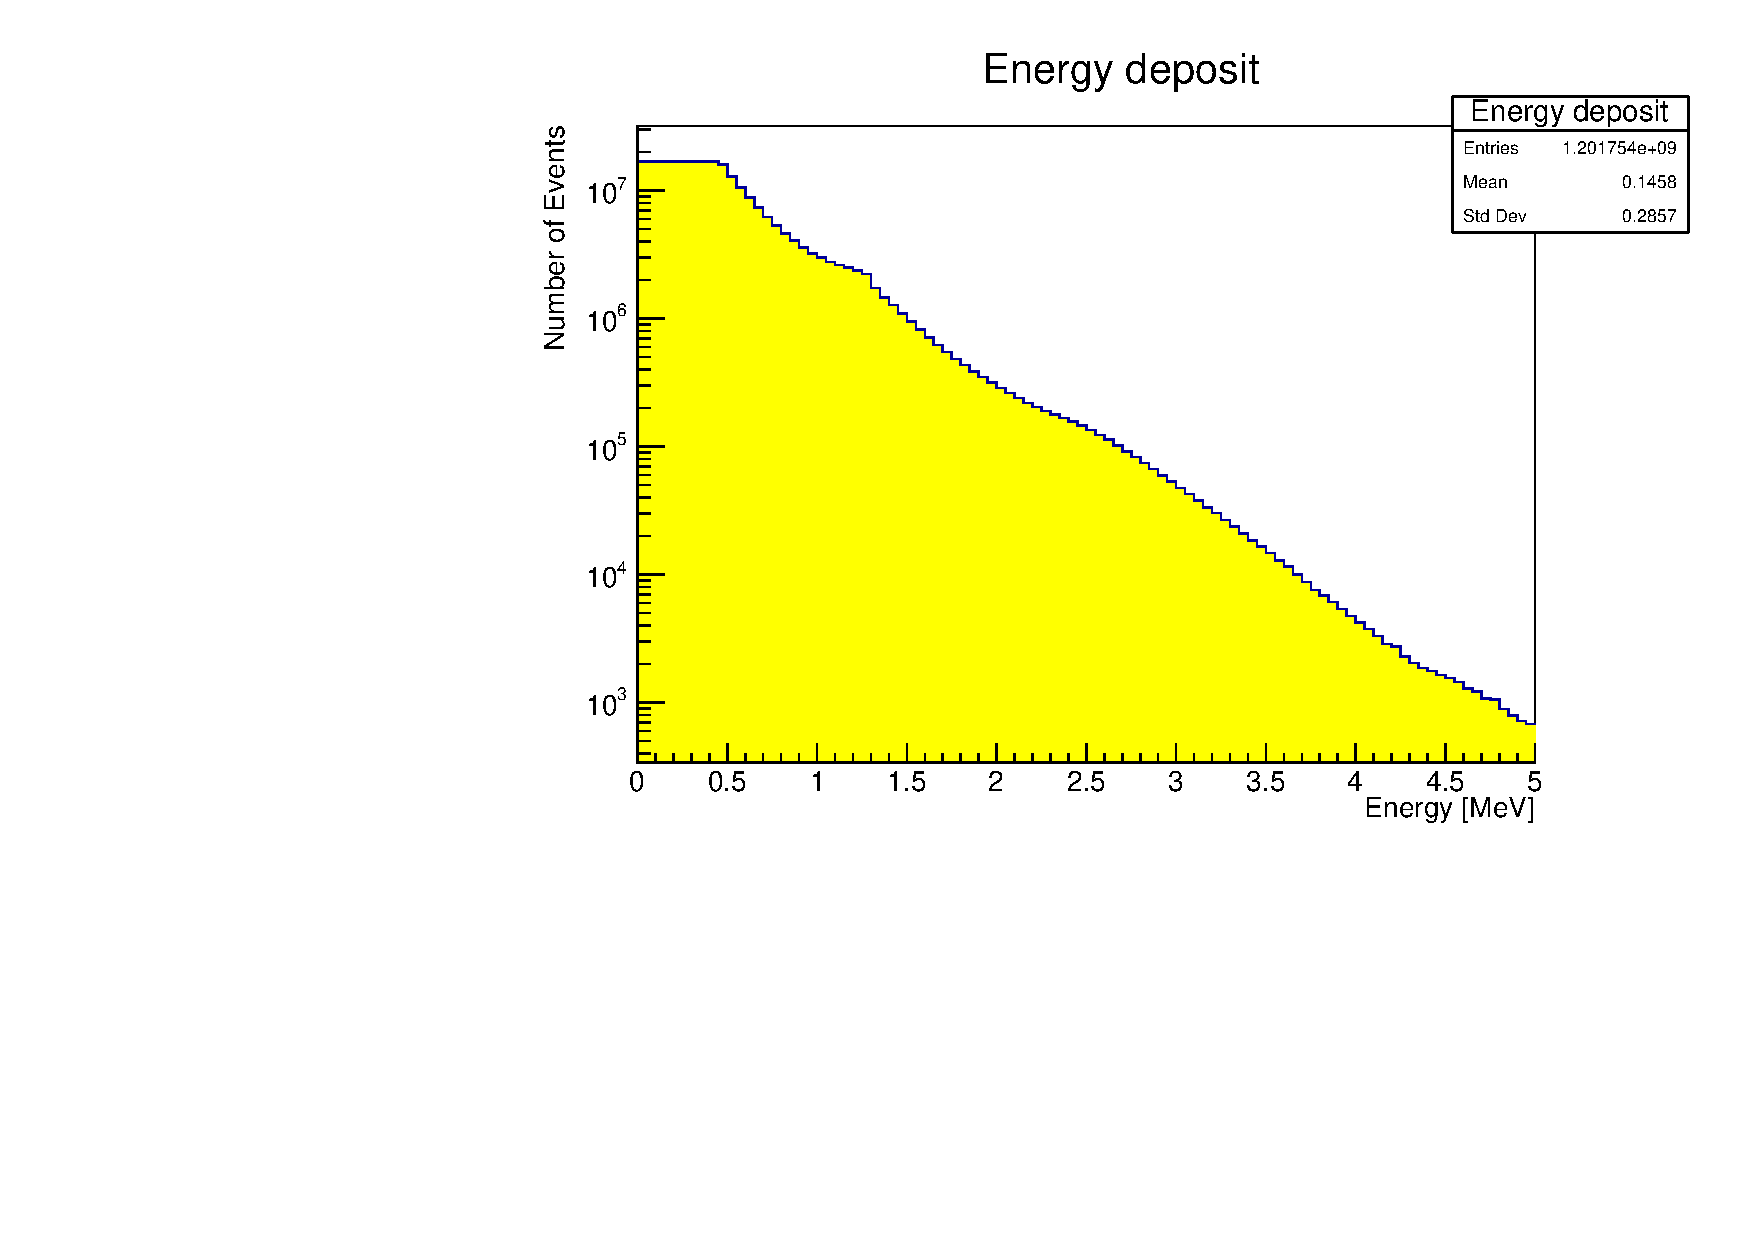
\includegraphics[scale=0.35]{Kap3/pi0_lead_electrons_plots_energy_hist.pdf}\label{fig:energy-lead-3}}

  \caption{Energy deposit in the lead plates of the calorimeter.}\label{fig:energy-lead}

\end{figure}

The energy deposit in the scintillator plates (\cref{fig:energy-scintillator})
and in the lead plates (\cref{fig:energy-lead}) show similar distributions for
all the three primary particles. The same happens to the step length, then, the
results of the Kolmogorov test would determine which cells have significant
different distributions in these two variables to be considered in the machine
learning implementation.

\begin{figure}[htb!]
  \centering

  \subfloat[\(e^-\) as primary particle.]{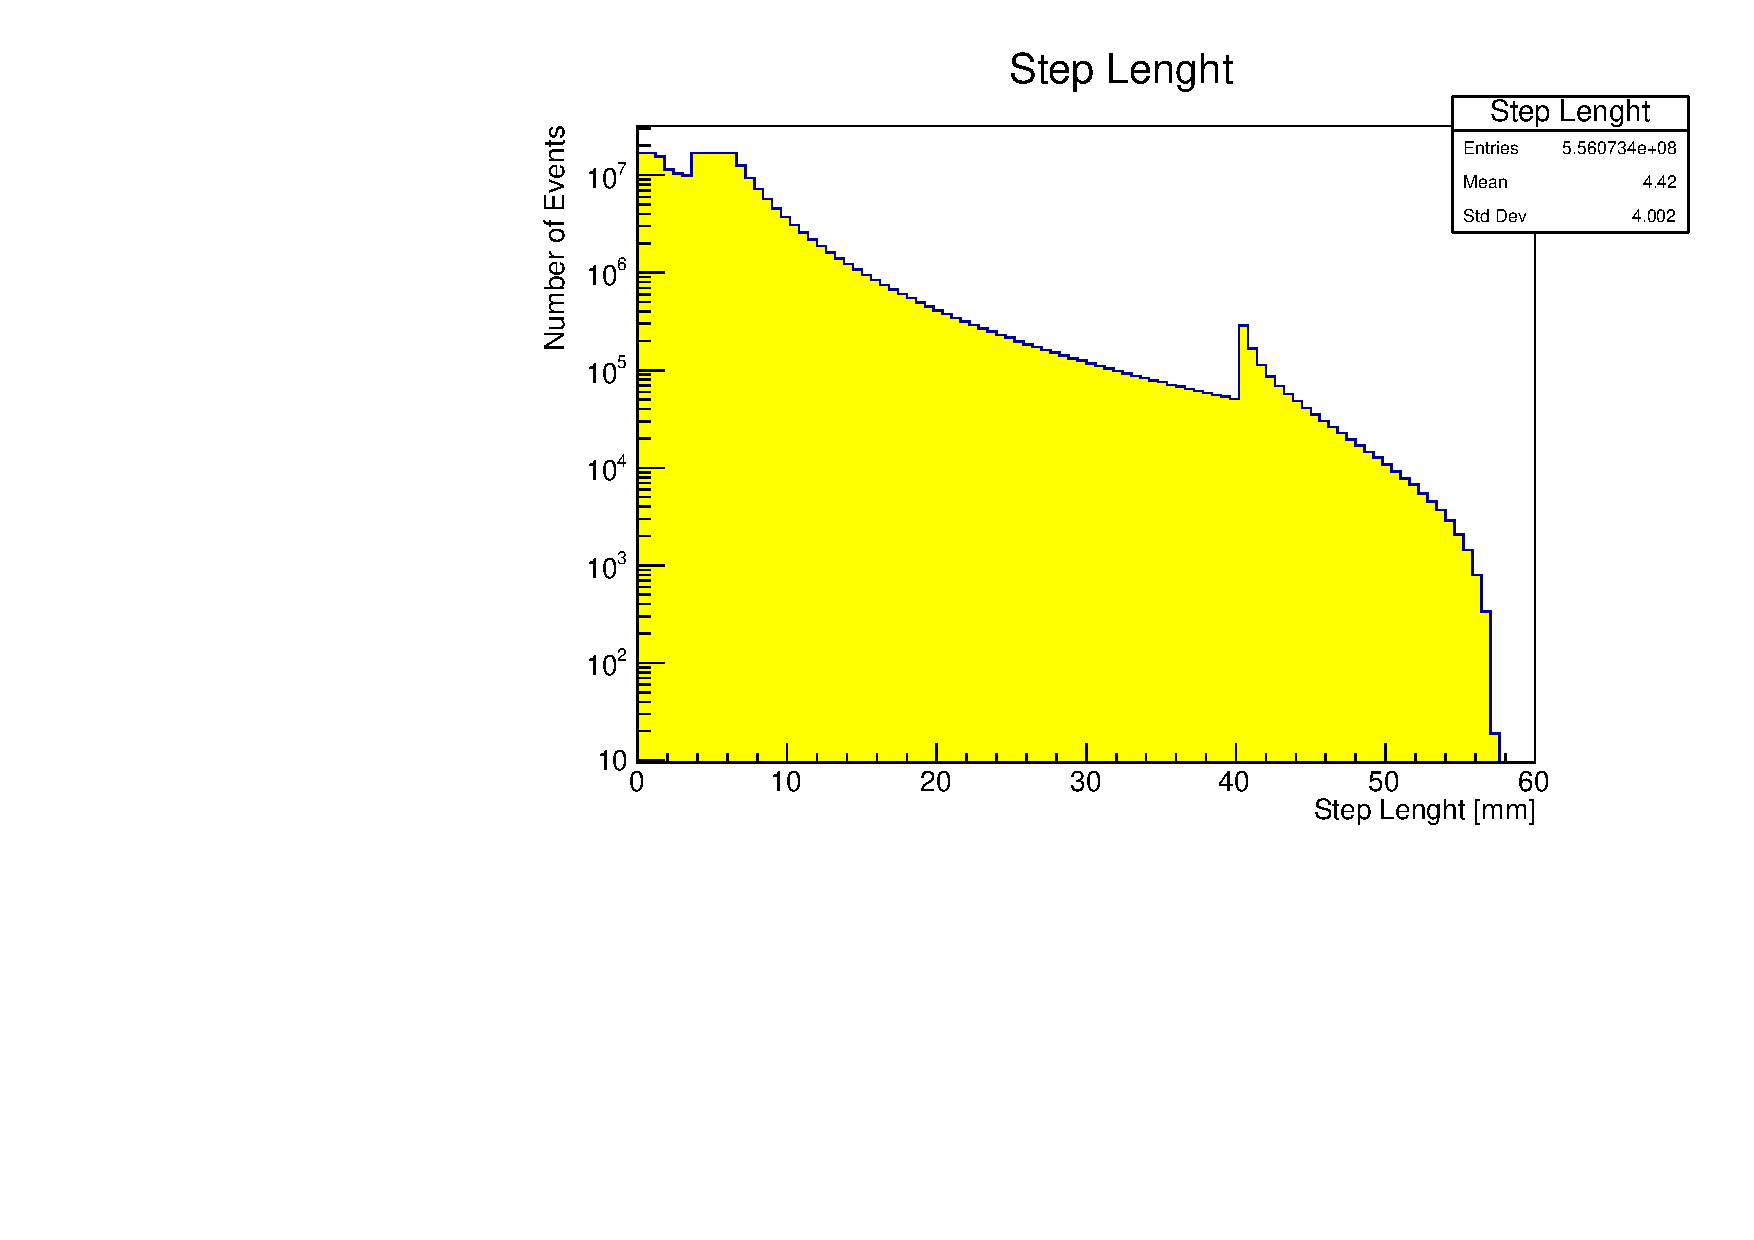
\includegraphics[scale=0.35]{Kap3/electron_scintillator_electrons_plots_step_lengt_hist.pdf}\label{fig:step-lengt-scintillator-1}}\hspace{1em}
  \subfloat[\(\gamma\) as primary particle.]{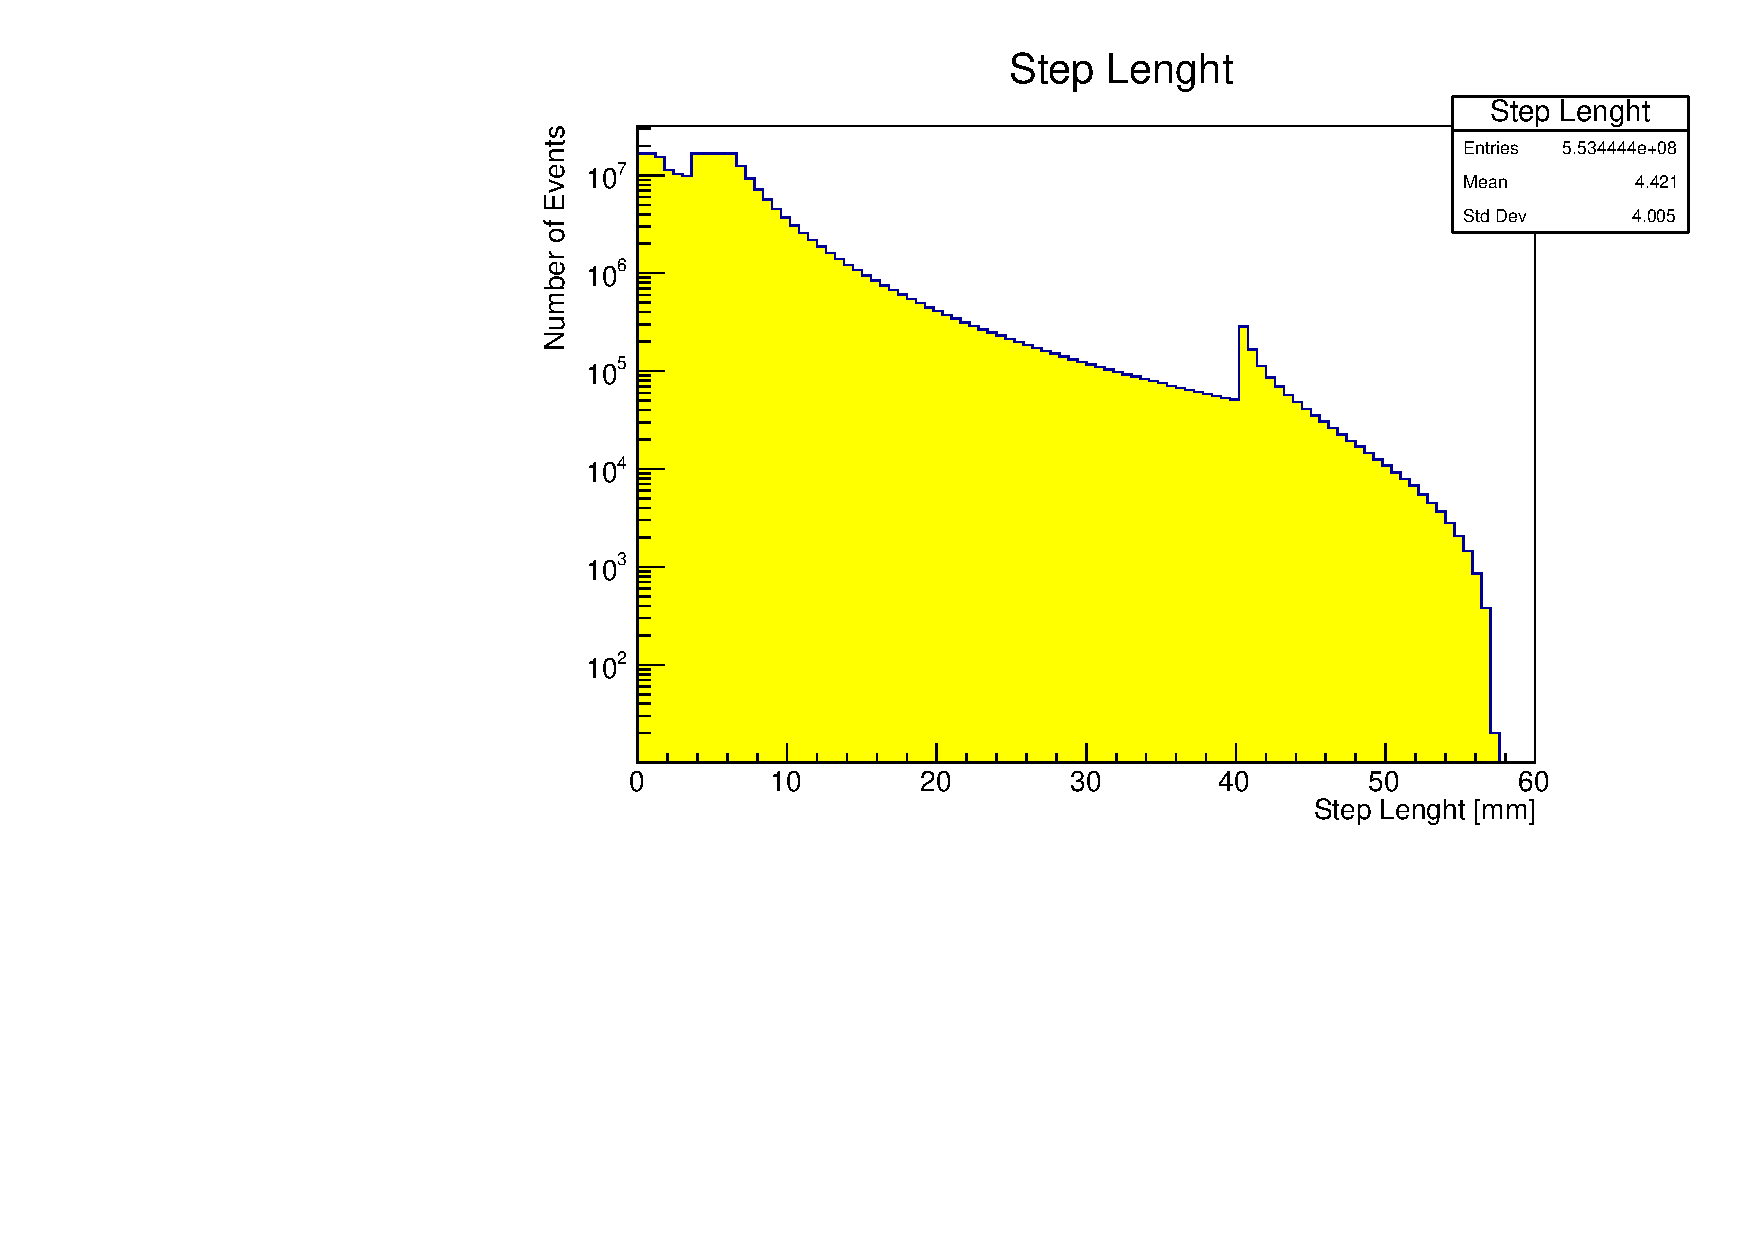
\includegraphics[scale=0.35]{Kap3/gamma_scintillator_electrons_plots_step_lengt_hist.pdf}\label{fig:step-lengt-scintillator-2}}\hspace{1em}
  \subfloat[\(\pi^0\) as primary particle.]{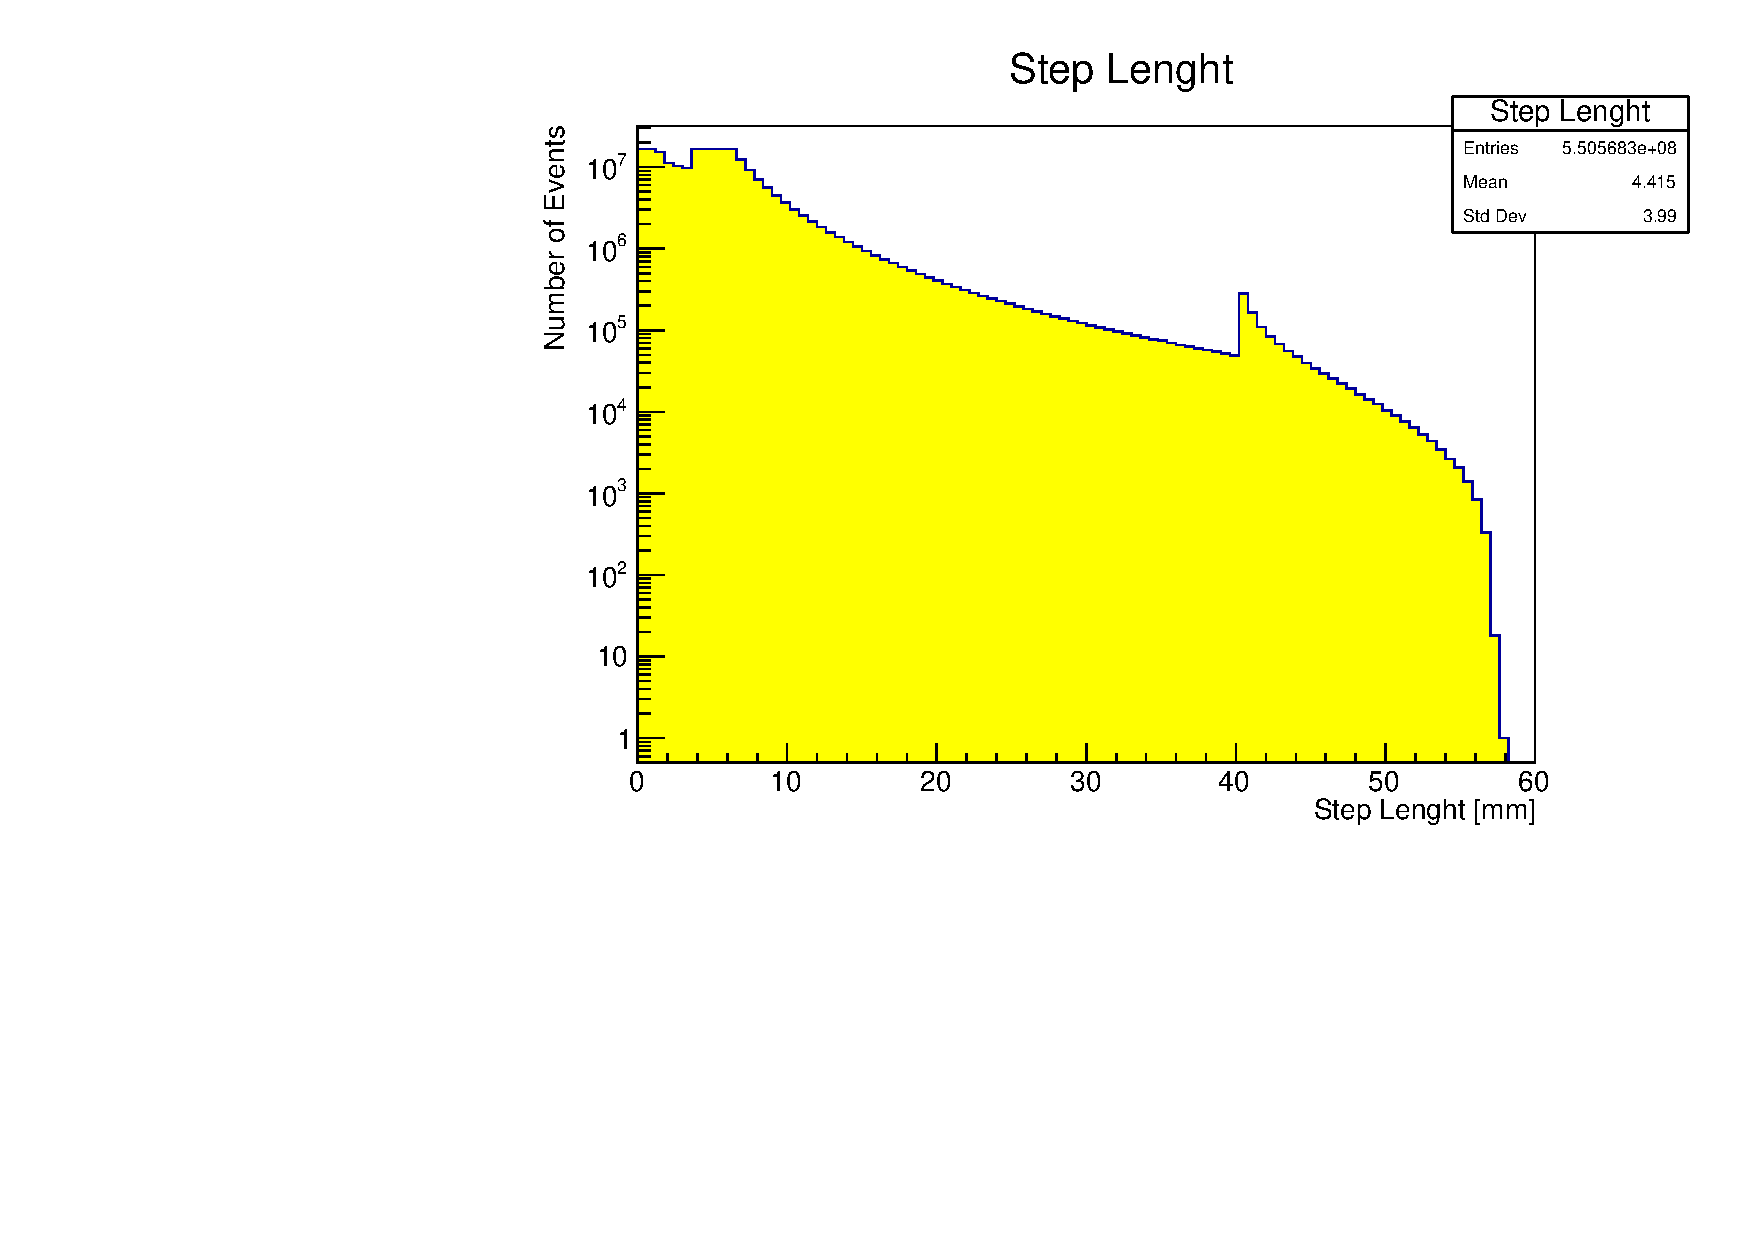
\includegraphics[scale=0.35]{Kap3/pi0_scintillator_electrons_plots_step_lengt_hist.pdf}\label{fig:step-lengt-scintillator-3}}

  \caption{Energy deposit in the scintillator plates of the calorimeter.}\label{fig:step-lengt-scintillator}

\end{figure}

After the Kolmogorov test, from a total of \(16056\) cells, \(14749\) were
tagged as significant for the number of photon created, \(15190\) for the
number of electron created, \(15122\) for the the energy deposit in the plates
and \(15122\) for the step length of the interaction.

\begin{figure}[htb!]
  \centering

  \subfloat[\(e^-\) as primary particle.]{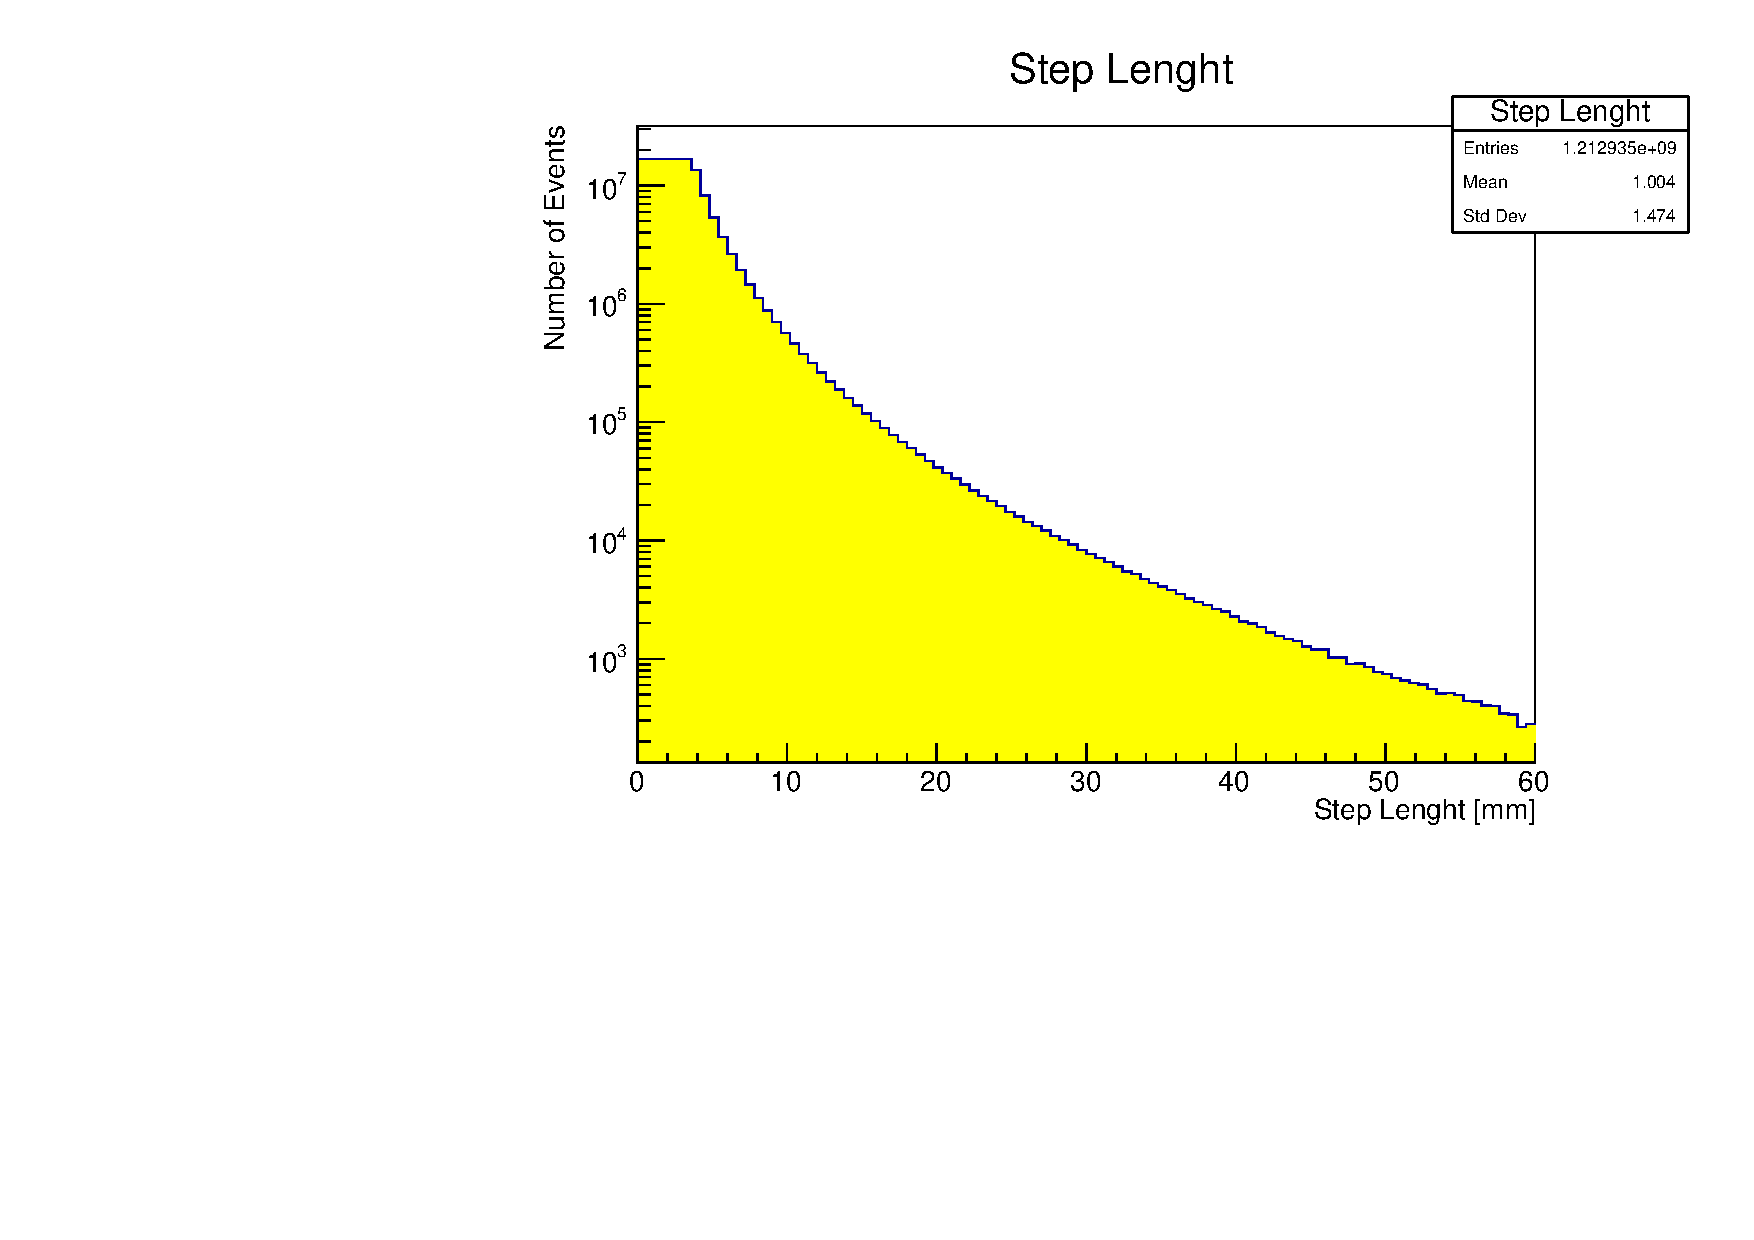
\includegraphics[scale=0.35]{Kap3/electron_lead_electrons_plots_step_lengt_hist.pdf}\label{fig:step-lengt-lead-1}}\hspace{1em}
  \subfloat[\(\gamma\) as primary particle.]{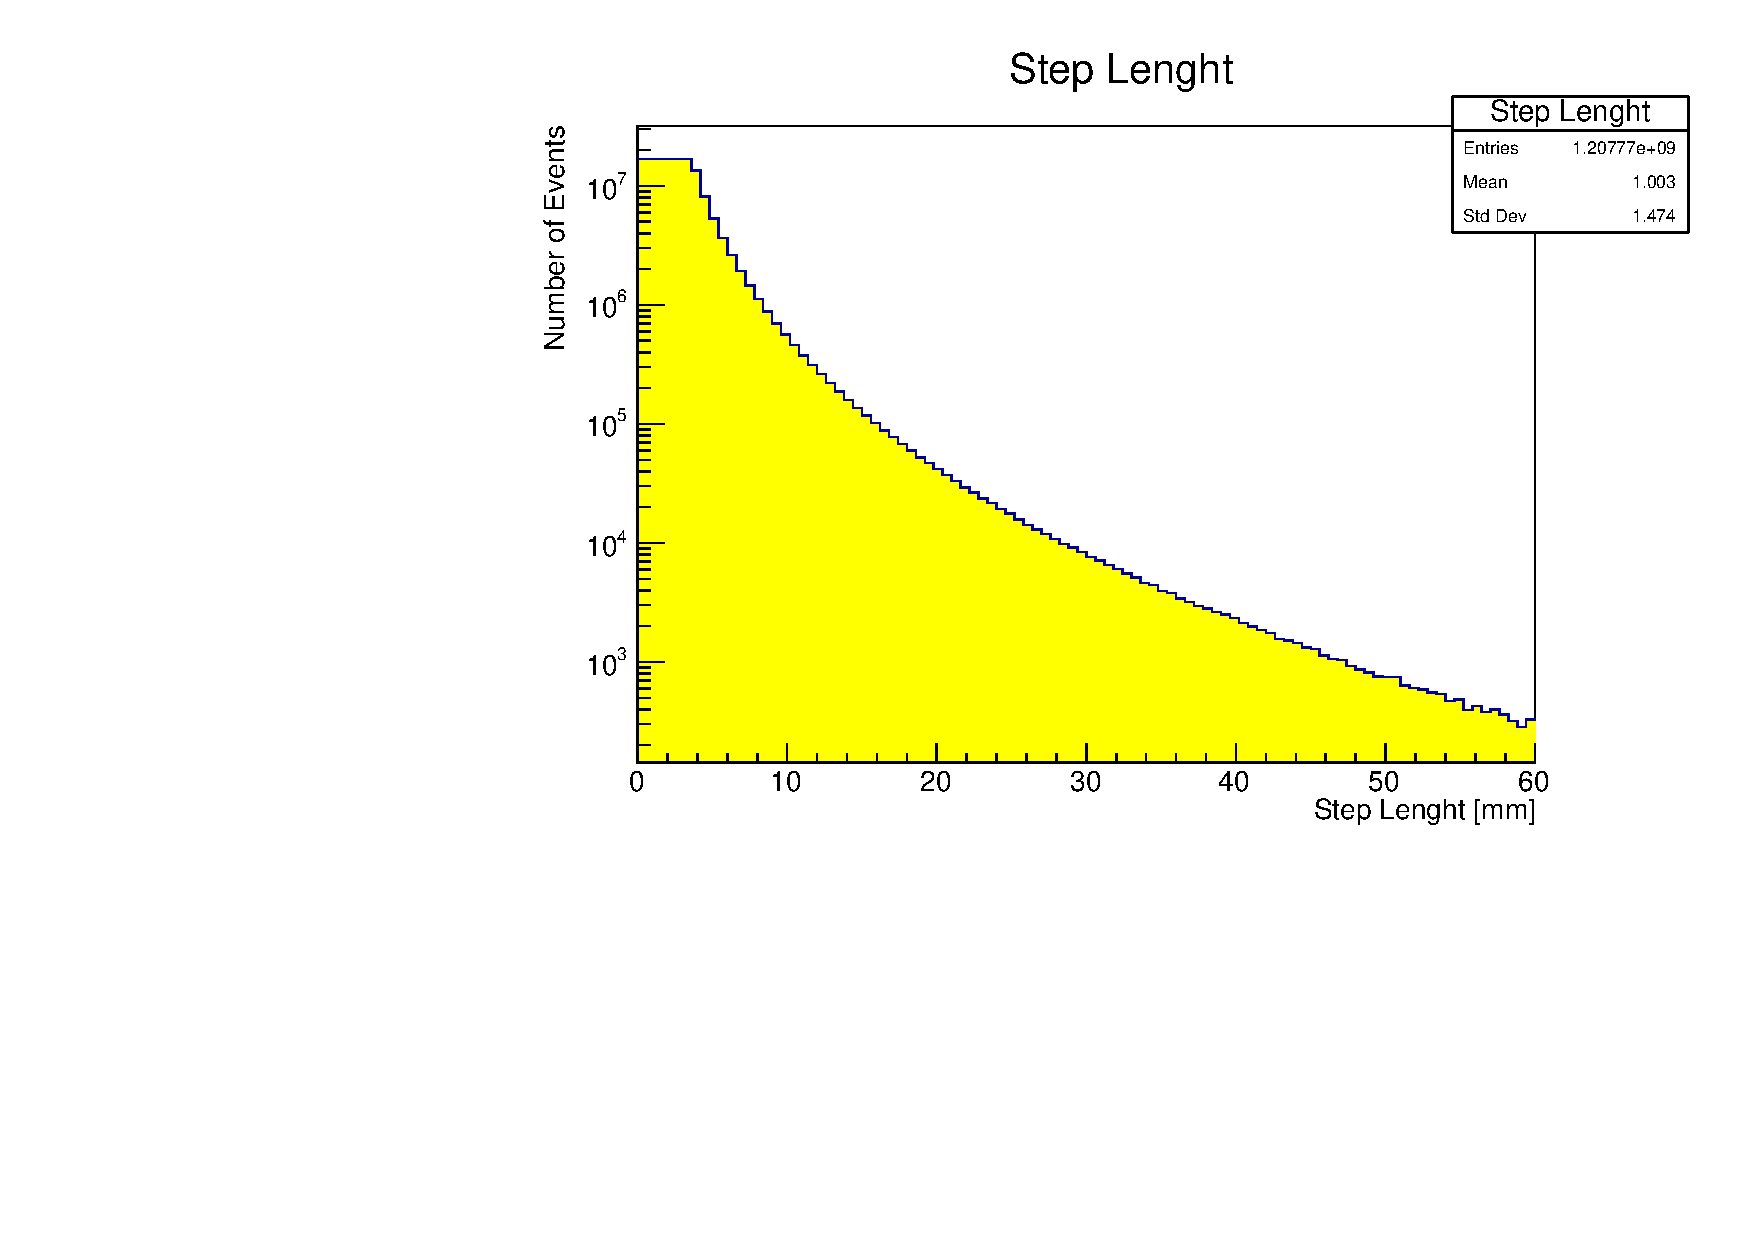
\includegraphics[scale=0.35]{Kap3/gamma_lead_electrons_plots_step_lengt_hist.pdf}\label{fig:step-lengt-lead-2}}\hspace{1em}
  \subfloat[\(\pi^0\) as primary particle.]{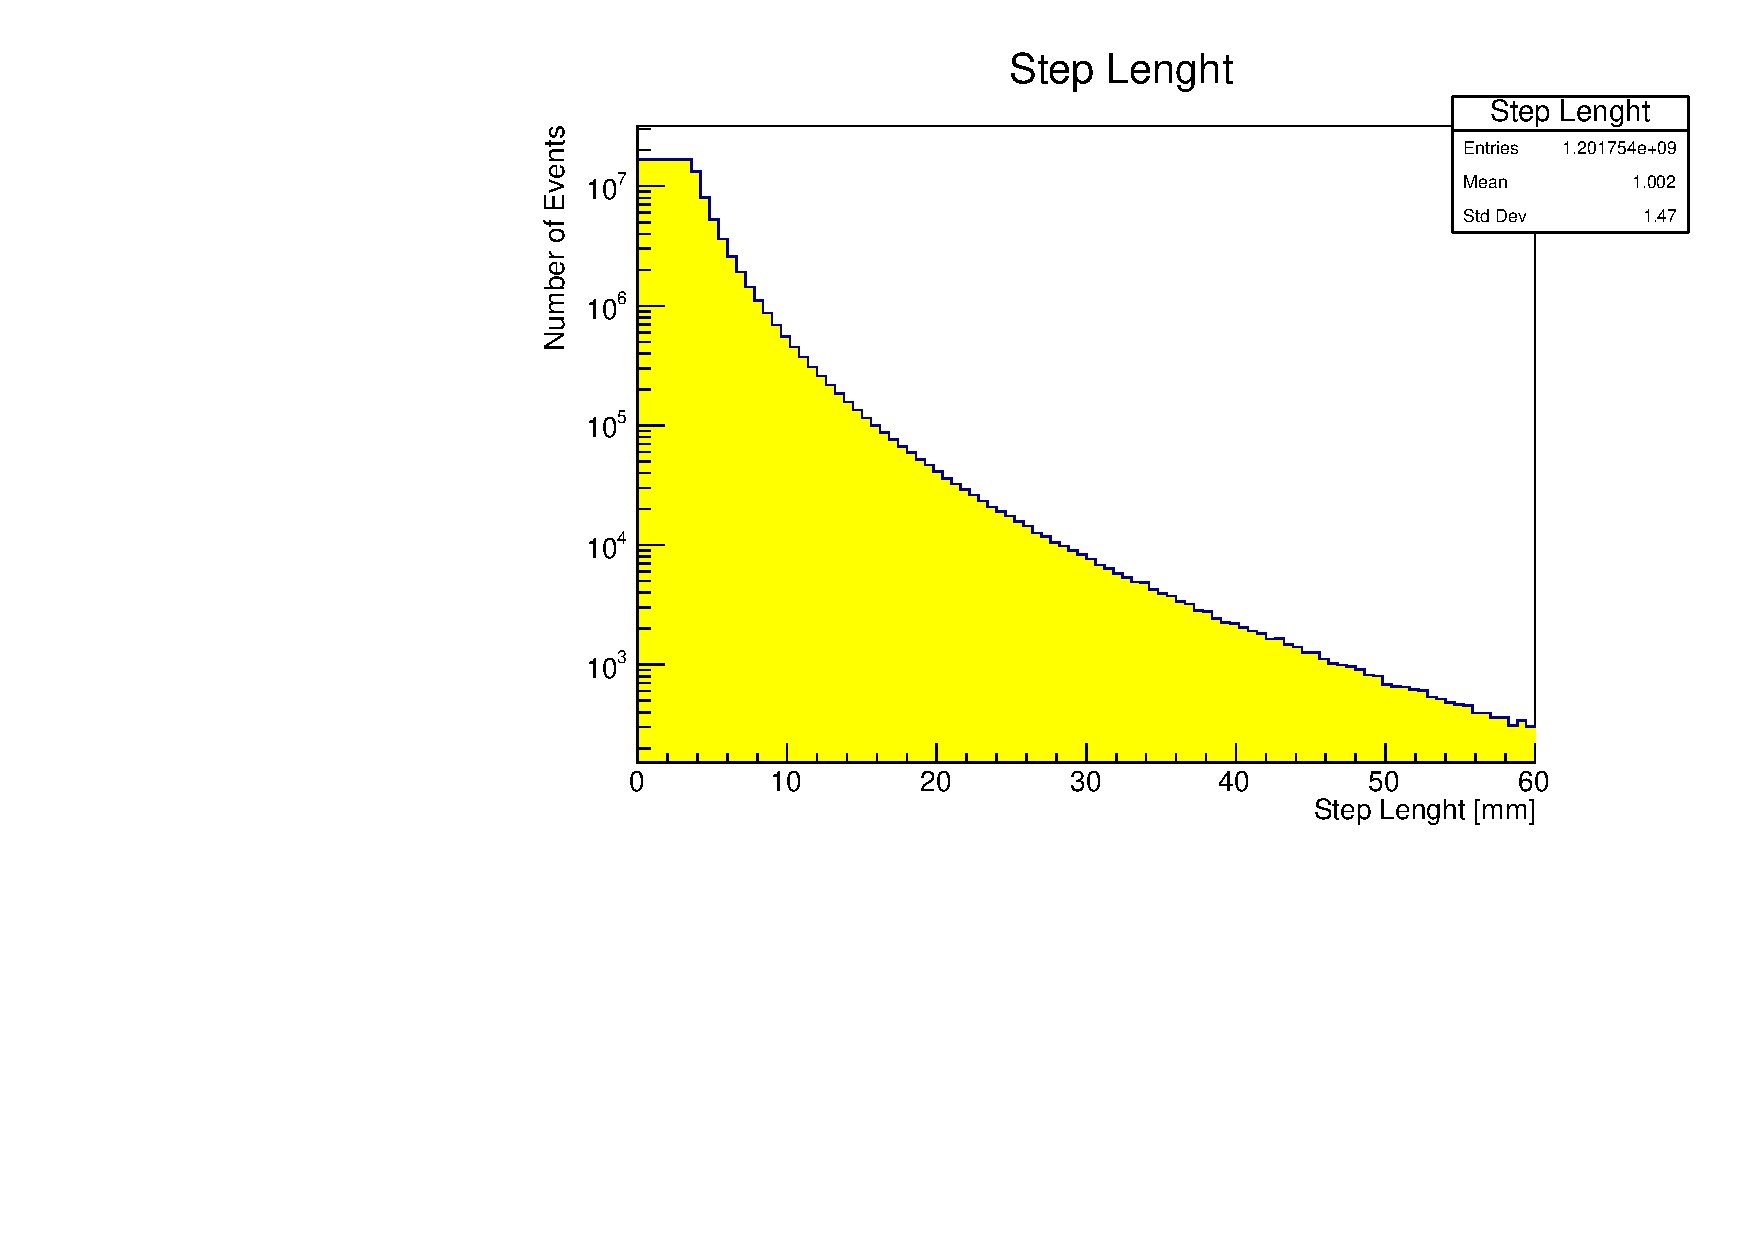
\includegraphics[scale=0.35]{Kap3/pi0_lead_electrons_plots_step_lengt_hist.pdf}\label{fig:step-lengt-lead-3}}

  \caption{Energy deposit in the lead plates of the calorimeter.}\label{fig:step-lengt-lead}

\end{figure}

Finally, the values resulting for the particle creation in the plates, as well
as the energy deposit and step length of the interactions were used as the
input of a machine learning implementation, using the multidimensional
classifiers, MultinomialNB, BernoulliNB, Perceptron, SGDClassifier and
PassiveAggressiveClassifier. The accuracy separating the events according to
the primary particle is shown in the \cref{tb:machine-learning-results}. From
this results, it can be noted that only the BernoulliNB classifier achieved
more than half of the correct answers separating the events, but still did not
get a good accuracy predicting the primary particle.

\begin{table}[hbt]
  \centering
  \begin{tabular}{c c}
    \textbf{Classifier} & \textbf{Result}\\
    \toprule
    MultinomialNB & 0.45\\
    \midrule
    BernoulliNB & 0.55\\
    \midrule
    Perceptron & 0.33\\
    \midrule
    SGDClassifier & 0.33\\
    \midrule
    PassiveAggressiveClassifier & 0.33\\
    \bottomrule
  \end{tabular}
  \caption{Accuracy of the machine learning methods.}\label{tb:machine-learning-results}
\end{table}

For the other methods, it can be seen that they do not predict correctly which
is the incident particle with the given input.
